\documentclass[manuscript]{acmart}
\usepackage[utf8]{inputenc}
%\usepackage{subfig}
\usepackage{balance} 
\usepackage{graphicx}
\usepackage{pifont} % for checkmark and crossmark
%\usepackage{cite}
\usepackage{xspace}
\usepackage{algorithmic}
\usepackage{algorithm}
\usepackage{caption}
\usepackage{subcaption} % for subcaption
\usepackage{url, hyperref}
\usepackage{xfrac}
\usepackage{wrapfig}
\usepackage{soul}
\usepackage{amsmath,amsthm}
\usepackage{multicol}
\usepackage{multirow}
%\usepackage{subfig} 
\usepackage{comment}
%\usepackage{todonotes}
\usepackage{xcolor,colortbl, supertabular}
\usepackage{layouts} % for computing textwidth
\usepackage{gensymb} % for degree symbol
%% Packages for coloring equations from Sibin paper
\usepackage{tikz}
\usetikzlibrary{backgrounds}
\usetikzlibrary{arrows,shapes}
\usetikzlibrary{tikzmark}
\usetikzlibrary{calc}
\usepackage[normalem]{ulem} % for strikeththrough

% Packages for the confusion matrix drawing
\usepackage{hhline}
\usepackage{collcell}

% To put text in a box
\usepackage{tcolorbox}

% for Q & A
\usepackage{enumitem}

% For subfig class
% \ifCLASSOPTIONcompsoc
% \usepackage[caption=false, font=normalsize, labelfont=sf, textfont=sf]{subfig}
% \else
% \usepackage[caption=false, font=footnotesize]{subfig}
% \fi
% \usepackage{epstopdf}
%%%%%%%%

% % For spacings
%\usepackage[subtle]{savetrees}
%%%%%%%%%%%%%%%%AUTHOR COMMENTS%%%%%%%%%%%%%%%%%%%%%%%%%%%%%%
\newif \ifdraft
\drafttrue % draft mode on, turns all comments on, DO NOT SUBMIT WITH THIS
%\draftfalse % draft mode off, turns all comments off

\newcommand{\akshay}[1]{\ifdraft \textbf{\sffamily\textcolor{purple}{[#1 -- Akshay]}} \else \fi}
\newcommand{\sumukh}[1]{\ifdraft \textit{\textcolor{magenta}{[#1 -- Sumukh]}} \else \fi}
\newcommand{\ashish}[1]{\ifdraft \textcolor{red}{#1 -- Ashish} \else \fi}
\newcommand{\ins}[1]{\ifdraft \textcolor{red}{#1} \else \fi}
\newcommand{\sibin}[1]{\ifdraft \textit{\textcolor{blue}{[#1 -- Sibin]}} \else \fi}
%%%%%%%%%%%%%%%%%%%%%%%%%%%%%%%%%%%%%%%%%%%%%%%%%%%%%%%%%%%%%%

\newcommand{\eg}{{\it e.g.,}\xspace}
\newcommand{\viz}{{\it viz.,}\xspace}
\newcommand{\Eg}{{\it E.g., }}
\newcommand{\etal}{{\it et~al.}\xspace}
\newcommand{\ie}{{\it i.e.,}\xspace}
\newcommand{\etc}{{\it etc.}}
\newcommand{\ci}{{\it (i) }}
\newcommand{\cii}{{\it (ii) }}
\newcommand{\ciii}{{\it (iii) }}
\newcommand{\civ}{{\it (iv) }}
\newcommand{\ca}{{\it (a) }}
\newcommand{\cb}{{\it (b) }}
\newcommand{\cc}{{\it (c) }}
\newcommand{\cd}{{\it (d) }}
\newcommand{\ce}{{\it (e) }}
\newcommand{\cf}{{\it (f) }}
\newcommand{\cg}{{\it (g) }}
\newcommand{\ch}{{\it (h) }}
%\newcommand{\ci}{{\it (i) }}
\newcommand{\cj}{{\it (j) }}
\newcommand{\ck}{{\it (k) }}
\newcommand{\cl}{{\it (l) }}
\newcommand{\cm}{{\it (m) }}
\newcommand{\cn}{{\it (n) }}
\newcommand{\co}{{\it (o) }}
\newcommand{\cp}{{\it (p) }}
\newcommand{\cq}{{\it (q) }}
%\newcommand{\note}{{\bf Note: }}
\newcommand{\cmark}{\ding{51}}
\newcommand{\xmark}{\ding{53}}
\newcommand{\cout}{$C_{\text{out}}$\xspace}
\newcommand{\aout}{$A_{\text{out}}$\xspace}
\newcommand{\tampered}{$S_{\text{tampered}}$\xspace}
\newcommand{\working}{$S_{\text{working}}$\xspace}
\newcommand{\couttampered}{$C_{\text{out,tampered}}$\xspace}
\newcommand{\coutworking}{$C_{\text{out,working}}$\xspace}

%% Table row coloring 
\newcommand{\ra}[1]{\renewcommand{\arraystretch}{#1}}
\colorlet{tableheadcolor}{gray!25} % Table header colour = 25% gray
\newcommand{\headcol}{\rowcolor{tableheadcolor}} %
\colorlet{tablerowcolor}{gray!25} % Table row separator colour = 
\colorlet{tablerowcolor2}{gray!12} % Table row separator colour = 10% gray
\newcommand{\rowcol}{\rowcolor{tablerowcolor}} %
\newcommand{\rowcollight}{\rowcolor{tablerowcolor2}} %


% Commands for Highlighting text -- non tikz method - copied from Sibin paper
\newcommand{\highlight}[2]{\colorbox{#1!17}{#2}}
\newcommand{\highlightdark}[2]{\colorbox{#1!47}{#2}}

\newcommand{\sol}{{PIRMedic}\xspace}

% For the blue circles in the overview picture
\definecolor{ultramarine}{RGB}{68,114,196}
\DeclareRobustCommand\circled[1]{\tikz[baseline=(char.base)]{\node[shape=circle,fill=ultramarine,inner sep=1pt] (char) {\textcolor{white} {#1}};}}


\AtBeginDocument{%
	\providecommand\BibTeX{{%
			Bib\TeX}}}

\begin{document}
\date{}
\title{Physics-based Fault Analysis for Commodity PIR Sensors}
\titlenote{PIRMedic was first introduced as a conference paper in ACM BuildSys~\cite{10.1145/3486611.3486658}. In this work, we expand upon on \sol and provide additional insights on the different classes of faults. We accomplish this by adding a threshold-based technique to study Class I and III faults (\S\ref{subsec:aout_quiet_times}) and including experiments using the threshold algorithm to distinguish between them by evaluation in a cafeteria (\S\ref{subsubsec:cafeteria}). We also study the impact of incremental failures on Class III faults giving insights into impact of gradual degradation on the \aout signal with incremental accumulation of dust(\S\ref{subsec:incremental_dust}). Additionally, we study the impact of different types of foreign particles such as paper and tape on the sensor performance (\S\ref{subsec:foreign_additional}). More generally, we include a quantitative study to compare the impact of various faults on sensor performance (\S\ref{subsec:quantify} and Table~\ref{tbl:fault_degree}). We also study the fault detection accuracy of \sol as a function of pre-deployment training dataset size (\S\ref{subsec:fail_detection}). Lastly, we have study the nature of \aout from ceiling-mount PIR sensors (Fig.~\ref{fig:round_lens}). We have also made some editorial changes by: \ca adding a goals subsection in \S\ref{sec:intro}, \cb updating other physics-related sensor failure related work~\cite{10.1145/3458864.3466869, 10.1145/3576842.3582386}, \cc adding a Frequently Asked Questions (FAQs) summarizing some of the common questions in the appendix and lastly \cd including a 3D visualization of the PIR sensor drawn in Tinker CAD and adding more text explaining the different sensor subsystems.}
% Add dept emails and affiliation
\author{Ashish Kashinath}
\email{ashishk3@illinois.edu}
\affiliation{%
	\institution{University of Illinois at Urbana-Champaign}
	\country{USA}
}
\author{Sibin Mohan}
\email{sibin.mohan@gwu.edu}
\authornote{Work done while affiliated with University of Illinois at Urbana-Champaign}
\affiliation{%
	\institution{The George Washington University}
	\country{USA}
}
\author{Akshay Nambi}
\email{akshay.nambi@microsoft.com}
\affiliation{%
	\institution{Microsoft Research}
	\country{India}
}

\author{Sumukh Marathe}
\email{sumukhm@umich.edu}
\authornote{Work done while affiliated with Microsoft Research India}
\affiliation{%
	\institution{University of Michigan}
	\country{USA}
}


\begin{abstract}
	Passive Infra-Red (PIR) sensors are ubiquitous and have applications ranging from automatic lighting and heating control in smart buildings,  towel dispensers in washrooms, security alarms (for intrusion detection) to human detection robots (for search and rescue). 
	%
	Unfortunately, PIR sensors are prone to failures during deployment due to reasons such as environmental damage, incorrect installation and component degradation among others that can lead to incorrect or faulty data. 
	%
	Currently, such failures are typically detected using either : \ca heavily engineered data-driven, statistical approaches that can have high false positive rates due to unseen data patterns or \cb expensive, unscalable methods that use additional hardware such as video cameras or a golden reference sensor.
	%
	In this work, we first create a \textit{taxonomy} for the most common PIR sensor failures and analyze these failures from the perspective of sensor physics.
	%
	We then present \sol --- a \textit{physics-driven, edge-based approach} to \textit{detect} and \textit{diagnose} the failures in a PIR sensor using an intrinsic hardware signal~\viz the analog output from the pyroelectric element in the sensor. 
	%
	Using this hardware signal in conjunction with frequency analysis and supervised machine learning methods, we obtain a high accuracy of $98-99 \%$ in failure detection and diagnosis. 
	%
	We evaluate our methods using \textit{multiple real-world deployments}, in four distinct locations, in different environment and usage conditions.    
\end{abstract}
%% Rights management information.  This information is sent to you
%% when you complete the rights form.  These commands have SAMPLE
%% values in them; it is your responsibility as an author to replace
%% the commands and values with those provided to you when you
%% complete the rights form.
%\acmYear{2021}\copyrightyear{2021}
%\setcopyright{acmlicensed}
%\acmConference[BuildSys '21]{ACM International Conference on Systems for Energy-Efficient Built Environments}{November 17--18, 2021}{Coimbra, Portugal}
%\acmBooktitle{ACM International Conference on Systems for Energy-Efficient Built Environments (BuildSys '21), November 17--18, 2021, Coimbra, Portugal}
%\acmPrice{15.00}
%\acmDOI{10.1145/3486611.3486658}
%\acmISBN{978-1-4503-9114-6/21/11}



%%
%% The code below is generated by the tool at http://dl.acm.org/ccs.cfm.
%% Please copy and paste the code instead of the example below.
%%
\begin{CCSXML}
	<ccs2012>
	<concept>
	<concept>
	<concept_id>10010520.10010575.10010577</concept_id>
	<concept_desc>Computer systems organization~Reliability</concept_desc>
	<concept_significance>500</concept_significance>
	</concept>
	<concept_id>10010520.10010553.10010559</concept_id>
	<concept_desc>Computer systems organization~Sensors and actuators</concept_desc>
	<concept_significance>500</concept_significance>
	</concept>
	<concept>
	<concept_id>10010583.10010750.10010751</concept_id>
	<concept_desc>Hardware~Fault tolerance</concept_desc>
	<concept_significance>500</concept_significance>
	</concept>
	<concept>
	<concept_id>10010147.10010257</concept_id>
	<concept_desc>Computing methodologies~Machine learning</concept_desc>
	<concept_significance>500</concept_significance>
	</concept>
	<concept>
	<concept_id>10010520.10010553.10010562</concept_id>
	<concept_desc>Computer systems organization~Embedded systems</concept_desc>
	<concept_significance>500</concept_significance>
	<concept>
	<concept>
	<concept_id>10010520.10010553.10010562</concept_id>
	<concept_desc>Computer systems organization~Embedded systems</concept_desc>
	<concept_significance>500</concept_significance>
	</concept>
	</ccs2012>
\end{CCSXML}
\ccsdesc[500]{Computer systems organization~Reliability}
\ccsdesc[500]{Computer systems organization~Sensors and actuators}
\ccsdesc[500]{Hardware~Fault tolerance}
\ccsdesc[500]{Computing methodologies~Machine learning}
\ccsdesc[500]{Computer systems organization~Embedded systems}
\keywords{Passive Infra-Red (PIR) Sensors, Occupancy Sensors, Fault Diagnosis, Fault Detection, Fault Isolation, Cyber-Physical Systems, Embedded Systems, Edge Computing, Edge ML, Reliability, Dependability, IoT}
\maketitle
\section{Introduction}
\label{sec:intro}

Cyber-Physical and IoT Systems such as smart homes, industrial control and healthcare systems often require the correct functioning of a myriad set of sensors. 
%IoT applications deployed in smart homes, industrial control and healthcare systems require the correct functioning of a myriad set of sensors. 
%
%The sensors allow such systems to measure their environment and, trigger computations and actions. 
% that are part of their intended design.
%
These sensors measure the surrounding environment in the form of either an arithmetic value (\eg temperature of 72\degree F) or a logical value (\eg presence or absence of smoke) and, trigger computations and actions.
% 
Typically, these sensor data measurements are used by data-driven IoT analytics pipelines (\eg Microsoft Azure IoT) to derive insights and make higher-level decisions. 
%The data from these sensors is used by IoT analytics pipelines to derive patterns, insights and make decisions.
%
%In this paper, we will be looking at a Passive Infra-Red (PIR) sensor.
%
One of the most versatile and ubiquitous sensors used in numerous modern applications is a Passive Infra-Red (PIR) sensor.
%
A PIR sensor is a discrete, electronic sensor that captures thermal radiation from human and human-like objects (\eg animals) to indicate occupancy in a region. %its field of view.
%
They are used in a wide-variety of environments -- \eg in offices to achieve energy savings in buildings (for automatic control of lighting and HVAC systems) and in safety-critical cyber-physical systems (CPS) like factory floors for intrusion detection.
%They are used in a wide variety of environments, from building automation to safety-critical systems such as factories. 
%{\bfseries Fig.~\ref{fig:pir_in_smart_building}} shows PIR sensors in a modern building, where it is used to achieve energy and operational cost savings~\cite{PricewaterhouseCoopers}. 
%
%Consequently, the correct operation of PIR sensors is critical to the quality and performance of many IoT deployments.
Naturally, these applications mandate the correctness and fidelity of data \ie the data being a faithful representation of occupancy.
%and trigger computations or actions as per application requirements.}
%
%\ashish{what generic class of sensor?characteristics functionality. applications, general problems. go to failures.lets look at pir. then go into pir}
%
%An example of using occupancy sensor in smart buildings is shown in {\bfseries  
%  \eg automatic control of lighting and HVAC systems) 
%to even safety-critical systems such as manufacturing systems. 
% \subsection{Motivation}

%Unfortunately, these sensors are prone to failures and degradation of physical components. 
%
Given the nature of PIR deployments in the wild : for instance in remote, manually inaccessible, harsh conditions (\eg assembly line of a factory), they are prone to failures and degradation of physical components.
%
% In the case of the PIR\footnote{We focus on PIR in this paper though our observations are broadly applicable.} 
%
% In the case of the PIR sensor, 
% These failures could result in false triggers or failure to capture real movements \eg conference room lights turning off or doors not opening in spite of occupancy . 
%
These failures could result in false triggers or a failure to capture real movements \eg assembly line failures in a factory, inaccurate estimation of wildlife counts, conference room lights turning off or even doors not opening in spite of occupancy.
%
Such sensor failures are often caused by intermittent sensor faults that can happen in any one of its internal physical components~\cite{chakraborty2018fall,marathe2021currentsense}.
%
% shown in {\bfseries Fig. \ref{fig:pir_system_teardown}}, ~\eg physical damage to the lens or condensation damage to the optical filter. 


%A passive infrared sensor (PIR sensor) is a discrete, electronic sensor that captures thermal radiation from human and human-like objects (\eg animals) to indicate the occupancy in its field of view. The output of PIR sensor is in the binary form, indicating \textit{the presence (or absence)} of an object\footnote{We use the terms obstacle, object and human object interchangeably in this paper}. They are used in a wide-variety of environments -- \eg in offices to achieve energy savings in buildings (for automatic control of lighting and HVAC systems) and in safety-critical cyber-physical systems (CPS) like factory floors for intrusion detection. Naturally, these applications mandate the correctness and fidelity of data \ie the data being a faithful representation of the presence (or absence) of an object.



%Despite surging in usage, it remains an unfortunate fact that PIR sensors are prone to false triggers as well as missing presence of objects. For example, it sometimes happens that lights in conference rooms to accidentally turn off despite motions and fail to turn on unless one waves their arms around aggressively for the sensors to capture motion. Phenomena such as these are caused mostly due to intermittent sensor faults. A system teardown of the PIR sensor is shown in Fig.~\ref{fig:pir_system_teardown} and faults can happen in any of these components~\eg physical damage to the lens or condensation damage to the optical filter.

% \begin{figure}[htbp] 
	% 	%%%%%%%%%%%%%%%%
	% 	% SMART BUILDING
	% 	%%%%%%%%%%%%%%%%
	% 	\begin{minipage}[t]{0.5\textwidth}
		% 		%\begin{figure}
		% 		\centering
		% 		%\begin{flushleft}
		% 		%\includegraphics[width=1.0\columnwidth]{figures/platform/pir-sensor-internals-combine-with-3d.png}
		% 		\includegraphics[width=0.8\textwidth]{figures/motivation/PIR-applications-in-smart-buildings.png}
		% 		%\end{flushleft}
		% 		\caption{\textbf{Applications of PIR sensor} in Smart Buildings.}
		% 		%\vspace*{-0.5\baselineskip}
		% 		\label{fig:pir_in_smart_building}
		% 		%\end{figure}
		% 	\end{minipage}%
	% 	%%%%%%%%%%%%%%%%
	% 	% END OF SMART BUILDING
	% 	%%%%%%%%%%%%%%%%
	% \end{figure}

%\begin{figure}
%%%%%%%%%%%%%%%%
% MOTIVATION FOR PHYSICS
%%%%%%%%%%%%%%%%
\begin{wrapfigure}{R}{0.5\textwidth}
	\centering
	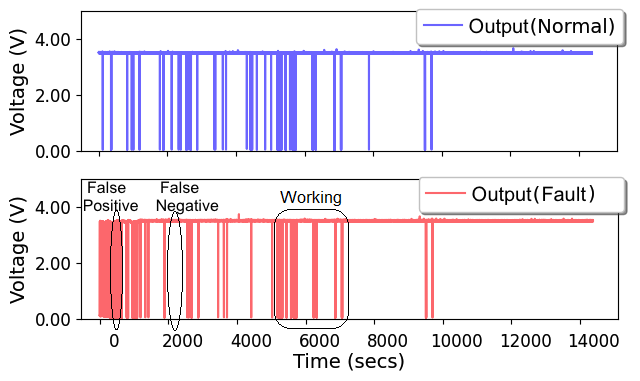
\includegraphics[width=0.5\textwidth]{figures/motivation/motivation-physics-technique.png}
	\caption{\footnotesize{Sensor Data} from a working PIR (top) and a faulty PIR (bottom). HIGH indicates no object, HIGH$\rightarrow$LOW transition indicates object.}
	\label{fig:occupancy_sensor_data}
\end{wrapfigure}
%%%%%%%%%%%%%%%%
% END MOTIVATION FOR PHYSICS
%%%%%%%%%%%%%%%%

% \begin{figure*}%[htbp]
	% 	%%%%%%%%%%%%%%%%
	% 	% SENSOR TEARDOWN
	% 	%%%%%%%%%%%%%%%%
	% 	\begin{minipage}[b]{0.25\textwidth}
		% 		\begin{flushleft}
			% 		%\begin{figure}
			% 		%\centering
			% 		%\includegraphics[width=1.0\columnwidth]{figures/platform/pir-sensor-internals-combine-with-3d.png}
			% 		%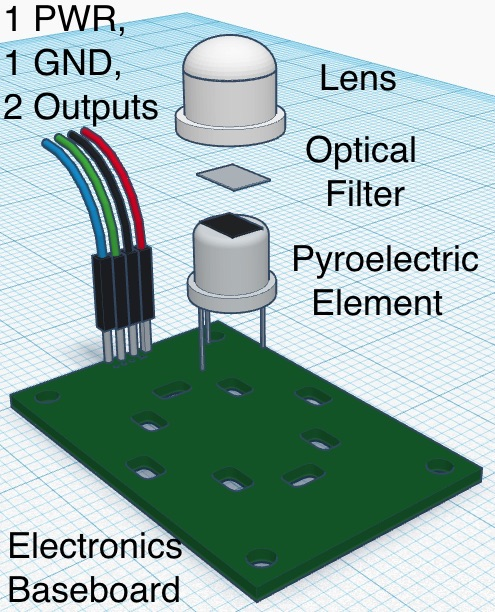
\includegraphics[height=1.5in]{figures/platform/3d_view_5-annotated.jpg}
			% 		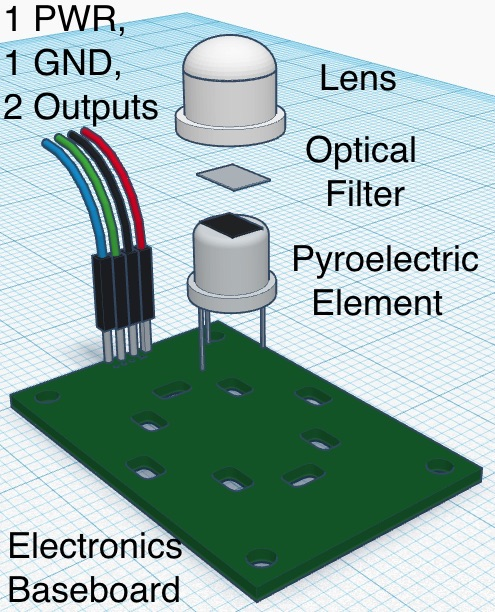
\includegraphics[width=0.9\textwidth]{figures/platform/3d_view_5-annotated.jpg}
			% 		\end{flushleft}
		% 		\caption{\textbf{PIR Sensor Teardown}}
		% 		%\vspace*{-0.5\baselineskip}
		% 		\label{fig:pir_system_teardown}
		% 		%\end{figure}
		% 	\end{minipage}%
	% 	%%%%%%%%%%%%%%%%
	% 	% END OF SENSOR TEARDOWN
	% 	%%%%%%%%%%%%%%%%
	% 	\hspace{5ex}
	% 	%%%%%%%%%%%%%%%%
	% 	% PIR SENSOR PIPELINE
	% 	%%%%%%%%%%%%%%%%
	% 	%\begin{subfigure}{0.48\textwidth}
	% 	\begin{minipage}[b]{0.60\linewidth}
		% 		%\begin{flushright}
		% 		\centering
		% 			\begin{subfigure}[t]{\textwidth}
			% 				\includegraphics[width=\textwidth,height=0.9in]{figures/platform/pir-block-diagram-2.png}
			% 				\caption{}
			% 				\label{fig:pir_sensor_pipeline}
			% 			\end{subfigure}\\
		% 			\begin{subfigure}[t]{\textwidth}
			% 				\includegraphics[width=\textwidth,height=0.7in]{figures/platform/sensys_workflow.png}
			% 				\caption{}
			% 				\label{fig:system_workflow}
			% 			\end{subfigure}
		% 		%\end{flushright}
		% 		\caption{\ca \textbf{Physics of the} PIR Sensing Pipeline, \cb \textbf{End-to-end workflow} of \sol for fault detection and diagnosis.}
		% 		\label{fig:pir_sensing_pipeline}
		% 	\end{minipage}
	% 	%\end{subfigure}%
	% 	%%%%%%%%%%%%%%%%
	% 	% END OF PIR SENSOR PIPELINE
	% 	%%%%%%%%%%%%%%%%
	% \end{figure*}    


%\begin{figure}[t]
%	\centering
%	\small
%	\begin{subfigure}[t]{0.5\textwidth}
	%		\centering
	%		\includegraphics[width=\textwidth]{figures/platform/pir-block-diagram-2.png}
	%		\caption{\textbf{PIR Sensing Pipeline} showing the physics.}
	%		\label{fig:pir_sensor_pipeline}
	%	\end{subfigure}\\
%	\begin{subfigure}[t]{0.5\textwidth}
	%		\centering
	%		\includegraphics[width=\textwidth]{figures/platform/sensys_workflow.png}
	%		\caption{\textbf{End-to-end Workflow} for performing data capture and fault analysis of PIR sensors.}
	%		\label{fig:system_workflow}
	%	\end{subfigure}
%\end{figure}

Currently, failures in PIR sensor deployments are usually addressed in one of the following two ways : \ca using an additional, auxiliary sensor such as a CCTV camera combined with image processing algorithms (say to validate the occupancy data) or \cb using high-grade PIR sensors that possesses additional capabilities such as ultrasonic sensors and intricate optics. This makes the sensor deployment very expensive. % with intricate optics and added capability such as ultrasonic sensors. 
In addition, deployments need to be refreshed periodically by replacing old sensors with new ones and the former are disposed off %trashed 
adding to both electronic waste and cost. A case in point is our university research building where the occupancy sensor deployed is a high-grade PIR sensor comprising both ultrasonic and infrared sensors, resulting in a \emph{total recurring cost of close to \$100000 every 10 years}\footnote{Our 4-floor building (with a total of 244 rooms and 24 aisle areas) has more than 300 occupancy sensors. Each PIR sensor costs \$300~\cite{hubbell_ADT1600WRP, hubbell_ATD2000CRP} with it being refreshed every 10 years, a worst-case recurring cost of \$90000 every 10 years, which is expensive.}.


\begin{comment}
	%%%%%%%%%%%%%%%%
	% MOTIVATION FOR PHYSICS
	%%%%%%%%%%%%%%%%
	\begin{wrapfigure}{L}{6cm}
		\centering
		\vspace{-10pt}
		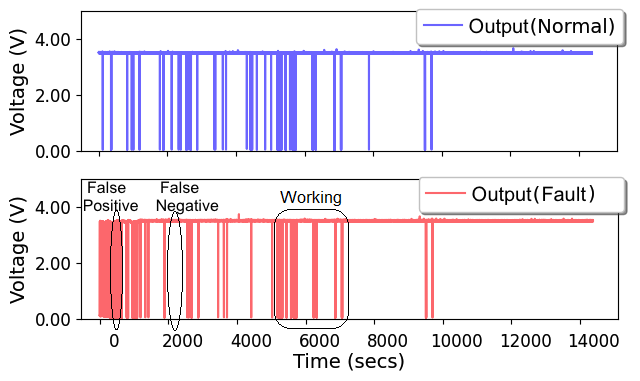
\includegraphics[width=0.4\columnwidth]{figures/motivation/motivation-physics-technique.png}
		\caption{\textbf{Occupancy Sensor Data} from a working sensor (top) and a degraded sensor with some dust deposited on the lens (bottom). The output follows negative logic \viz 0 -- object, 1 -- no object.}
		%\vspace*{-1.0\baselineskip}
		\label{fig:motivation_physics}
		\vspace{-10pt}
	\end{wrapfigure}
	%%%%%%%%%%%%%%%%
	% END MOTIVATION FOR PHYSICS
	%%%%%%%%%%%%%%%%
\end{comment}

Crucially, \textit{current approaches do not diagnose the cause of failures or perform any analysis of sensor performance}, that can be valuable for IoT %smart building 
engineers during maintenance, repair and testing. For example, in one of our deployments, we observed that failed or degraded sensors can exhibit unpredictable behavior \eg they can work temporarily for a period of time and then fail sometimes. {\bfseries  Fig.~\ref{fig:occupancy_sensor_data}} shows a plot of output data from the sensor vs. time for both a working sensor and a faulty sensor (defective lens) over a period of 4 hours.
% \footnote{Internals of PIR sensor are covered in \S\ref{sec:approach}}. 
In this plot, a transition from HIGH$\rightarrow$LOW denotes a person coming into the field of view %an obstacle 
and a value of HIGH indicates that there is no person. %obstacle.
We observe that the faulty sensor works intermittently and at other times, can miss a person (false negative) or incorrectly flag the presence of a person (false positive).
%In {\bfseries  Fig.~\ref{fig:occupancy_sensor_data}}, we see that the faulty sensor missed a person %n obstacle 
%
%around 6:45 pm, whereas the same faulty sensor worked correctly through 6 pm. These failures can evade failure detection schemes that are purely data-driven since the data looks good up to 6:45 pm.
%
Missing a person can cause a potentially critical failure in applications such as door opening systems or emergency shutdowns on factory floors.
%
We show that accurate detection of such failures is possible by \textit{characterizing the internals of the sensor.}
%
%Additionally, physics-based reliability techniques can be used to augment AI/ML-based cloud IoT analytics pipelines.% 
%
%\eg Microsoft Azure IoT.
%In addition, extra sensors also require extra power using power packs such as CU-300A~\cite{hubbell_power_pack_cu300a} that only add to the cost.
%While both these approaches partially offset the issue albeit at a high cost, from an engineering standpoint, it makes the reliability of the composite system to be dependent on the additional sensor (\eg camera) as well that of the PIR sensors -- thereby reducing the failure probability. 

% In a nutshell, current solutions to faulty/incorrect sensor data \ca make the deployment expensive (additional auxiliary or high-grade sensors), \cb add to potential electronic waste (sensors are refreshed periodically) and \cc they do not diagnose failures. Thus, we need to look for alternative approaches.

\begin{comment}
	\begin{tcolorbox}%[top=0.05pt,bottom=0.05pt,boxsep=0pt,toptitle=0.1ex,bottomtitle=0.1ex]
		[left=0.05pt,right=0.05pt,top=0.05pt,bottom=0.05pt,boxsep=0pt,toptitle=0ex,bottomtitle=0ex,sharp corners]
		{\bfseries Summary:} Existing solutions for reliability in IoT sensors: \ci require additional, auxiliary sensors, \cii do not diagnose failures, and \ciii add to electronic waste, resulting in large recurring cost.
	\end{tcolorbox}
\end{comment}
% \subsection{Our Study and Results}

\emph{Our solution, \sol detects and diagnoses failures of PIR sensors by characterizing the physics of sensing} \viz the fresnel lens optics and the pyroelectric effect. % and analyzing the various subsystems in action through the sensing pipeline. 
%
To keep the cost of the deployment low, \sol is implemented on the edge platforms of the deployment and targets commodity PIR sensors.
%
In this process, %the process of characterizing the physics, 
we \emph{devised a taxonomy of key failures for aiding diagnosis and repair.} 
%This does not require any additional auxiliary sensor and can thus be used to develop low-cost solutions to validate the correctness and fidelity of sensor data.

Specifically, we demonstrate that a signal intrinsic to PIR sensors~\viz the \textit{intermediate analog output from the pyroelectric element, referred to as \aout} ({\bfseries Fig.~\ref{fig:pir_sensing_pipeline}}) can be used for %has 
fault detection and diagnosis. % capabilities. % and performance monitoring capabilities. 
%
We utilize this signal to derive information about reliability of the PIR sensor platform as well as to perform an analysis into the different failure modalities. \textit{To the best of our knowledge, this is the first edge-based, low-cost approach to use an intrinsic signal (\aout) for fault detection and diagnosis of PIR sensors.} We analyze the behavior of \aout in detail, under %various conditions -- both in a controlled setting in the lab as well as in
practical deployments, with realistic occupancy
%(both before and during pandemic~\cite{doi:10.1056/NEJMe2002387})
over a wide variety of observed failures. 
%Note that we do not use any auxiliary or high-grade sensor and thus this approach can be used to develop low-cost solutions to validate the correctness and fidelity of sensor data.

\noindent \textbf{Summary of Contributions:}
%\vspace{-5pt}
\begin{enumerate}[leftmargin=*]
	\itemsep0pt
	\item \textit{From physics to failures:} We use the working of a PIR sensor to understand the process of object detection and infer the key points where failures could lead to incorrect sensor data,
	\item \textit{Failure taxonomy:} We study the impact of different failures on the sensor performance and systematize the key failures into a failure taxonomy. We also provide a quantitative method to study the severity of failures.
	% Note that while the taxonomy is PIR-specific, the core principles can be applied to other sensors as well.
	% and analyze the performance under different failure scenarios.
	
	\item \textit{Non-intrusive, online fault detection and diagnosis:} We present an online technique (does not require any disassembling), \emph{implemented at the edge}, for failure detection as well as diagnosis by utilizing the intermediate, analog output from the pyroelectric element in the PIR sensor (\aout). 
	%
	%The technique is completely online (does not require any disassembling) and is implemented at the edge device. 
	%
	%We demonstrate the use of \aout as a proxy to classify between faulty and working sensors.
	%
	%In addition to classification, we also show how \aout can be used to diagnose the failures \ie failure identification.
	%
	% ({\bfseries Fig.~\ref{fig:system_workflow}})
	\item \textit{Insights from Real-world Deployments:} We show the efficacy of the proposed techniques using a deployment of 15 PIR sensors in four practical occupancy scenarios over a period of 3 months.
	%(elevator, lobby of a building and at starbucks)
	% across two countries
	%(India, US)
	% -- both before and during the SARS-CoV-2 (Covid-19) pandemic~\cite{doi:10.1056/NEJMe2002387}. 
	% We use our techniques to detect and analyze faults occurring in practice.
\end{enumerate}

% \textbf{Impact:} Due to lack of standard designs of PIR sensors, we propose all the sensor vendors to include the \aout signal in all PIR sensor design standards to aid in the reliability of PIR sensors. This enables low-cost edge-based fault detection and diagnosis.% to be implemented at the Edge at low cost and minimal electronic waste.
% \ashish{say that its not real-time but it is online and computing is on the edge and not on backend clouds.}

\begin{comment}
	\subsection{Assumptions}
	\quad \underline{\bfseries Target System:} We consider PIR sensor deployments that are: \ca large in scale, \cb deployed remotely (making manual checking of faults hard), \cc consisting of low cost and \cd commodity off the shelf (COTS) sensors, such as those in modern smart buildings.
	%in that comprise of a large number of low-cost sensors that can degrade or fail. 
	%\ins{Being low-cost, these sensors have low compute or storage capabilities.}
	
	\underline{\bfseries Choice of sensor:} As our work leverages the \aout signal present in a PIR sensor, we require a PIR sensor that allows access to \aout either directly or indirectly by reworking the sensor such as ~\cite{PIR_sensor_eval}. While this limits the scope of our work, our framework can form the basis for manufacturers and IoT engineers for leveraging the rich information in \aout for inclusion in future designs.
	%Commercial occupancy sensors are of 4 different types of technologies : \ci Microwave antenna-based, \cii Ultrasonic-based, \cii Passive Infra-Red (PIR) or \civ Photocell (PC) based. Among these four technologies, PIR is the most commonly used, the cheapest, available from the largest number of vendors and also used in our buildings both in India and in the US. Thus, we chose PIR-based occupancy sensors for our analysis.
	
	\underline{\bfseries Existence of ground truth:} We perform our analysis of the occupancy patterns by gathering data from multiple different sensors, some of which can fail or degrade. However, we assume that not all sensors fail simultaneously as it enables us to separate physics of failed sensors from physics of working sensors. This is a reasonable assumption due to the large-scale nature of deployment.
	
	\underline{\bfseries Security of sensor values:} We perform our analysis of sensors at the edge, and assume that the sensor data are not tampered with using attacks such as Man-in-the-Middle attacks (MitM) or using software vulnerabilities in the edge platform.
\end{comment}

\noindent \textbf{Goals:}

\begin{enumerate}[leftmargin=*]
	\itemsep0pt
	
	\item {\itshape Detect failures:} Sensors can give faulty data due to the incorrect operation of various physical components involved in the sensing process. We seek to detect and isolate such failed sensors. %data that is not a faithful representation of the physical phenomenon.
	%
	
	\item {\itshape Diagnose failures:} In addition to detecting failures, we perform failure diagnosis to identify the cause of the failure. We use domain-knowledge of the sensing physics and our understanding of how different failures can impact the physics. This aids in repair and performing quality-control checks.
	%
	
	\item {\itshape Edge-based solution:} \sol is tailored for edge platforms (Raspberry Pi, Arduino Microcontrollers) that are interfaced directly to multiple sensors, say via GPIO. %\st{Being low-cost, these sensors have low compute or storage capabilities.}
	Edge-based reliability solutions allows us to reject data from faulty sensors in IoT deployments thus saving the cost of both \ca the edge to cloud network bandwidth and \cb cloud compute consumed by faulty data.
	%
	
	\item {\itshape Target Audience:} \sol benefits two sections of the community: \ca engineers developing and deploying IoT/Edge computing for occupancy sensors (\eg Smart Buildings), \cb manufacturers of occupancy sensors can use the insights from this work towards future PIR sensor hardware designs.
	
	%We first present the background, physics of the PIR sensor and our failure taxonomy. Next, we present details about the intrinsic hardware signal and analyse its behavior under the failure scenarios. Thereafter, we deploy our sensors in the wild for evaluation and conclude with lessons learnt from the real-world failures.
\end{enumerate}

\begin{comment}
	Sensors are the bridge between the compute domain and the physical domain. They provide a manifestation of the physical domain to the compute domain wherein the computation is then be performed. The result of this computation is then utilized to make changes to the physical domain. For example, when a user moves his palm under a faucet with an in-built sensor, it triggers a signal to open a valve that pours water onto his palms. This closed loop of $physical\_environment \rightarrow sensor \rightarrow compute \rightarrow actuator \rightarrow physical\_environment$, seen in all sensing systems excludes reliability measures such as failure detection and sensor drift. As a result, we currently piggyback techniques such as data-driven anomaly detection \cite{hill2010anomaly} and schemes as calibration \cite{maag2018survey} to existing systems to achieve reliability and confidence in the data.  Additionally, present techniques for hardware fingerprinting apply to a restricted class of sensors - analog sensors, which operate by periodically sampling a quantity of interest and where the voltage variation between the on and off states are high enough to be characterized. 
	
	% In this work, we integrate failure detection as a first class citizen in the sensing process by expressing it as a function hardware characteristics of the sensor. 
	
	In this paper, we present an automated, low-cost approach to fault detection in digital sensors, performed at the edge, without user intervention. We perform this by analyzing sensors which are outside the purview of the \textit{Fall-curve} \cite{chakraborty2018fall} technique. As sensors vary in nature by the phenomena being sensed, leading to different physics of operation, and hardware signals, there is no single silver bullet to detect faults. Instead, we present a suite of techniques based on most commonly found faults in the wild. %For example, different sensors use different physical principles to sense different kinds of physical variables such as temperature, pressure, and humidity among others. Additionally, due to the varying underlying principles, they also have different electronic and/or mechanical components.
	
	
	\newenvironment{myquotation}{\setlength{\leftmargini}{1.5em}\quotation}{\endquotation}
	\begin{myquotation}
		\noindent\textit{We present a principled approach to making digital sensors "reliable" - overcoming the challenges of capturing fall curve \cite{chakraborty2018fall} and finding alternative approaches to capture the hardware fingerprint of the sensor.}
	\end{myquotation}
	
	\noindent \textbf{Scope} We consider digital sensors out there are low cost, used in large scale, and are deployed in remote and harsh environments. From an application standpoint, we looked at sensors that are used in environmental monitoring.
	
	
	% \noindent \textbf{Our Approach}  Our approach entails using a \textit{systems} approach and thus requires us to understand the different systemic signals present in such sensors. We emphasize that these signals are disparate from the data that is being measured, making it independent of the environment and unique for a type of sensor. Examples of such signals include warm-up behavior, current consumption of different components during the sensing process, voltages at various intermediate points in the sensor circuitry before, during and after sensing and so on. In turn, identifying such signals requires us to understand the different components present in the sensor. It is to be noted that we need not understand every single electronic component in the sensor going all the way down to discrete circuit components as such an approach is neither scalable nor feasible. Furthermore, with increasing sophistication and reliability of manufacturing technology and the integrity checks in place at the fabrication, failures in the electronics are better handled by the conventional integrated circuit testing practices \cite{weste1985principles}. Instead, we analyze failures on a macro level at the granularity of a \textit{subsystem}. Our focus is on \textit{subsystems} that are prone to fail in the common case as discerned from failure reports and interaction with industry collaborations \cite{}. Broadly, our approach consists of four steps : \ci Studying and understanding physics of functional sensors, \cii Analyzing the different physical blocks present in the sensor, \ciii Identifying points of failure in each of the blocks, and \civ Devising techniques to monitor the blocks for failures.
	
\end{comment}
\section{Related Work} 
\label{sec:related}

%\hl{moved this section here and renamed it -- Sibin.}

%\section{Sensor Reliability : State of the Art}
%% BEGINNING OUTLINE 
% Current research in PIR sensors can be categorized into:
% \begin{itemize}
%     \item Time-series fault detection
%     \item PIR-specific related work
%     \item $A_{out}$ based PIR work
%     \item $A_{out}$ extended for fault detection
% \end{itemize}
%% END OF OUTLINE

\begin{comment}
\begin{table*}
	\centering
	%\hrulefill
	\caption{Overview of related work in the space of sensor fault detection}
	%\resizebox{\textwidth}{!}{
	\begin{tabular}{p{2cm} | p{2.5cm}p{4cm}p{1cm}p{3cm}p{3cm}}
		%\begin{tabular}{p{1.25cm}p{1cm}p{1.5cm}p{1.5cm}p{1cm}}
		\hline
		\bfseries \textsc{State of the Art} & 
		\bfseries \textsc{Approach} & 
		\bfseries \textsc{Remarks} & 
		\bfseries \textsc{Cost} & 
		\bfseries \textsc{Practicality} & 
		\bfseries \textsc{Notes} \\
		\hline \hline
		
		\rowcolor{gray!20} Khalastchi~\etal~\cite{} & 
		Data-driven + Model-based & 
		Requires suspicious patterns capturing the correlation of sensors. Applies to only stuck/drift faults. & 
		Moderate & 
		Shown on a single system &
		DS/ML \\
		
		Joerger and Pervan~\etal~\cite{} &
		Control Theoretical (Kalman Filter) &
		Monitoring state estimation errors &
		High &
		Shown in simulations only &
		Linear Dynamical systems \\
		
		\rowcolor{gray!20} Liu~\etal~\cite{} &
		Data-driven + Statistical filtering/recovery &
		Used for data errors such as timing, formatting and outliers &
		Moderate, heavy pre-engineering &
		Shown on a single system &
		Data recovery/cleaning and not fault diagnosis is the goal \\
		
		Ayadi~\etal~\cite{}, Elnahrawy~\etal~\cite{}, Koushanfar~\etal~\cite{}, Murphree~\etal~\cite{}, Ni~\etal~\cite{}, Niggemann~\etal~\cite{}, O'Reily~\etal~\cite{}, Power~\etal~\cite{}, Rashid~\etal~\cite{}, Sharma~\etal~\cite{}, Subramaniam~\etal~\cite{}, Wu~\etal~\cite{} &
		Data-driven environmental model &
		&
		&
		&
		\\
		
		\rowcolor{gray!20}Khoussainova~\etal~\cite{}, Krishnamachari~\etal~\cite{}, Ni~\etal~\cite{}, Sheng~\etal~\cite{}, Tolle~\etal~\cite{} &
		Estimation-based methods &
		&
		&
		&
		\\
		
		Maag~\etal~\cite{}, Whitehouse~\etal~\cite{}, Tang~\etal~\cite{}, Dorffer~\etal~\cite{}, Wang~\etal~\cite{}, Saukh~\etal~\cite{}, Xiang~\etal~\cite{}, Yan~\etal~\cite{} &
		Calibration-based methods &
		&
		&
		&
		\\
		
		\rowcolor{gray!20} Chakraborty~\etal~\cite{}, Liu~\etal~\cite{} &
		Hardware-based techniques &
		&
		&
		&
		\\
		
		
		
		
		\hline 
	\end{tabular}\\
	\vskip1pt 
	\quad \raggedright 
	$^1$ called inter-arrival time for sporadic and aperiodic flows
	%}
	\label{tbl:flow_para}
	\vspace{-1.5\baselineskip}
\end{table*}
\end{comment}


% \begin{table}
% %\begin{wraptable}{R}{8cm}%[ht]\small
% 	%\renewcommand{\arraystretch}{1.1}
% 	\vspace{-\baselineskip}
% 	\centering
% 	\footnotesize
% 	\caption{{\bfseries Physics-based sensor failure detection \& diagnosis} Approaches}
% 	%\vspace{-10pt}
% 	\begin{tabular}{p{2.25cm} p{2.5cm} p{2.5cm}}
% 		\hline %\\
% 		\textsc{\bfseries Aspect} & \textsc{\bfseries Fall Curve} & \textsc{\bfseries CurrentSense}\\
% 		\hline\hline
% 		\rowcolor{gray!20} \multicolumn{2}{l}{\bfseries Lens Subsystem}\\
% 		Lens dislodged \newline (Class I) & Lens cap suffers partial or complete dislocation \eg physical impact with a foreign object, degradation of bonding,~\etc \\
% 		Lens deformed \newline (Class II) & Lens cap suffers physical damage in-place \eg deformation, puncture,~\etc \\
% 		Lens covered \newline (Class III) & Lens cap gets physically obstructed by foreign particles \eg dust, paper or tape \\
% 		\hline
% 		\rowcolor{gray!20} \multicolumn{2}{l}{\bfseries Pyroelectric Subsystem} \\
% 		Optical filter \newline damage (Class IV) & Damaged by environmental factors~\eg oil condensation\\
% 		\hline
% 		\rowcolor{gray!20} \multicolumn{2}{l}{\bfseries Electronic Subsystem} \\
% 		Electronic faults \newline (Class V) & Hardware failures~\eg short circuits, floating outputs~\etc \\
% 		% Thermal Faults & Pyroelectric element can degrade or age and can give imperfect output\\
% 		\hline
% 	\end{tabular}
% 	\label{tab:pir_faults}
% 	%\vspace{-10pt}
% 	\vspace{-\baselineskip}
% %\end{wraptable}
% \end{table}

Current solutions for failure detection and diagnosis in sensors fall into one of three categories -- \ca Data-driven techniques, \cb Calibration-based techniques and \cc Fingerprint-based techniques.

\textbf{Data-driven techniques.} Prevalent research efforts have largely focused on data-centric approaches (rule-based or anomaly detection), where historical data %(ranging from days to years) 
of the sensor is analyzed and a fault is identified if the data is out of bounds of the expected behavior~\cite{rashid2016collect, 10.1145/3365871.3365872}.  Sharma~\etal~\cite{10.1145/1754414.1754419}, proposed a multiplicative seasonal ARIMA time series model for fault detection, where the parameter captures periodic behavior in the sensor data. % measurement time series. 
The downside of temporal analysis methods is that
they are prone to false positives and are not feasible in long-term
deployments. Wu~\etal~\cite{4262542} used a spatial mining-based approach that uses spatial correlation between neighboring sensors to detect anomalies. Additionally, techniques such as Ayadi~\etal~\cite{7505190}, Murphree~\cite{7589589} and Power~\etal~\cite{10.1145/3365871.3365872} require significant labeled data as it models only the environment and does not model the sensor physics. Estimation-based methods model normal sensor behavior leveraging spatiotemporal correlation and probabilistic models such as Bayesian or Gaussian distributions~\cite{10.1145/1140104.1140114} and they work well in homogeneous environments. In a nutshell, the key challenge with data-driven techniques is that it relies on rules and patterns in the sensed data.
We argue that for PIR sensors since the data is non-periodic and dependent on deployment scenarios (\eg people counting in Starbucks,   
animal detection in forests, etc.), \textit{it is non-trivial to detect faults by just analyzing sensor data.} Further, this requires significant manual efforts and tailor-made rules to detect faults, and can eventually have high false positives due to unseen data patterns. Additionally, data-driven techniques do not provide information about the specific nature or degree of failure in the sensor. As a result, they do not aid in the process of developing repair strategies. This is also seen in works such as Tawakuli~\etal~\cite{tawakuli2023experience}, that discusses the repercussions of missing data to be of two types -- \ca isolated missing data and \cb sequence missing data. They develop a domain-independent, dataset-independent, hybrid imputation strategy that can give better estimation accuracy by looking at six real-world datasets such as AirQuality and NASDAQ time-series data. Tawakuli~\etal~\cite{Tawakuli2022TransformingID} describes a generic edge-cloud IoT-based preprocessing framework targeting AI pipelines. The framework comprises steps such as data cleaning and feature engineering, and can leverage \sol to assist in cleaning data associated with faulty PIR sensors. In summary, data-driven techniques, while scalable, often entail substantial labeling efforts, leading to high costs, and can exhibit low accuracy due to their dependence on custom rules and patterns. Moreover, they provide no guidance on correcting faulty sensors, as they disregard the underlying physics of sensing.

\textbf{Calibration-based techniques.} These techniques rely on the presence of an additional (reference) sensor, either to perform periodic calibration~\cite{whitehouse2002calibration, 8405565} or carrying additional information in a different domain space.  \Eg using a camera to cross-check the data of a PIR sensor~\cite{tang2017occupancy}. Numerous algorithms have been developed for performing calibration such as blind calibration~\cite{7472216, 7495010}, collaborative calibration~\cite{10.1145/2737095.2737113, 10.1145/2185677.2185687} and transfer calibration~\cite{article_nose}. Agarwal~\etal~\cite{Agarwal2021ANA} uses temperature and power consumption data to infer if a HVAC is faulty or working. It relies on the correlation between the two individual data streams from auxiliary sensors~\viz smart meters and temperature sensor. By studying such a relationship between multiple sensors, Agarwal~\etal~\cite{Agarwal2022ANA} provide a optimization framework to minimize the number of sensors required to sense a facet such as occupancy. Their framework uses fault tolerance information in their framework and, in such a setting, \sol can be used to minimize the number of sensors in a Building Management System (BMS), thereby lowering operational costs and improving efficiency. Huchuk~\etal~\cite{huchuk2021data} develop a machine learning model based on data from thermostats to predict set points overrides that happen across a set of buildings, helping create more energy efficiency schemes. They note that using building-level indoor conditions will help create more energy efficient schedules and \sol can aid in improving the accuracy of such systems. However, all of these approaches that use reference sensors are expensive and lacks scalability for large IoT deployments. % or those in developing countries.%A majority of the current solutions for fault diagnosis in sensors are data-driven approaches using time-series fault detection~\cite{rashid2016collect, niggemann2015data}, where the nature of the data (\ie the final sensor output) is used to derive the status of the sensor as either working or failed. In addition, there exists solutions that rely on the presence of an additional (reference) sensor, either to perform periodic calibration~\cite{whitehouse2002calibration, 8405565} or carrying additional information in a different domain space.  \Eg using a camera to cross-check the data of a PIR sensor~\cite{tang2017occupancy}.  In addition, using reference sensors is an expensive strategy that does not scale well for larger deployments.

\textbf{Fingerprint-based techniques.} %Sensor failures can occur due to numerous reasons, from electronic component failures, improper installation to environmental factors such as dust and extreme temperatures. Recent works have focused on analyzing the underlying physics of the sensor and its hardware characteristics to determine sensor faults~\cite{chakraborty2018fall, marathe2021currentsense,10.1145/3458864.3466869}. 
Chakraborty~\etal~\cite{chakraborty2018fall} develop a sensor signature~\viz ``Fall Curve'' that measures a sensor's voltage response when the power is turned off, to detect faults in periodic on-off based analog sensors. 
%
The Fall Curve characterizes the parasitic capacitance and hardware circuitry of the sensor. Crucially, Chakraborty \etal show this signature is unique for every sensor type and is independent of the environment. They demonstrate that this approach works well for sensors that have very little or no warm-up time and work in a periodic on-off fashion. 
%
Furthermore, Chakraborty \etal \cite{chakraborty2018fall} point out to the fact that extending this approach to digital sensors where one doesn't have direct access to the analog signal is challenging. Additionally, Fall Curve is complex in sensors having low value of operating voltages and lack periodicity in the sensing mechanism. Our work concerns this design space of exploring faults in discrete-valued PIR sensors. PIR sensors are challenging since in addition to being discrete valued, the internal analog signal~\viz output from the pyroelectric element has a very low value. 
%
Similarly, Tambe~\etal~\cite{10.1145/3458864.3466869} show a variant of Fall Curve~\ie ``Fall Time'' of the analog signal can detect faults and drifts in phototransistor components of the sensor.
However, both Fall Curve and Fall Time signatures do not work on certain types of sensors including PIR, that operate under low voltages and are event-triggered. Marathe~\etal~\cite{marathe2021currentsense} show that analyzing the current profiles of a digital sensor can provide insights into component failures especially in electro-mechanical sensors. However, this approach is limited to power-hungry digital sensors. % that are power-hungry.
%
Gupta~\etal~\cite{10.1145/3576842.3582386} develop a Verified Telemetry SDK (VT-SDK) constructed on robust sensor fingerprinting algorithms and demonstrate fault detection on multiple sensors ranging from air pollution to pressure sensors.
%
There are other hardware-based techniques such as Liu~\etal~\cite{Liu_Huang_Luo_Harkin_McDaid_2019} that detects electronic faults by developing additional circuits inspired by the biology of neurons.
%
In summary, fingerprint-based techniques have been applied to sensors such as air pollution, smoke, and soil temperature and moisture sensors but have not been extended to PIR sensors.

%Our idea is inspired by the recent sensor fingerprinting approaches that exploits hardware signals to characterize the sensor and detect faults in them. Specifically, our work on PIR sensors addresses the challenge of diagnosing faults in non-periodic, discrete-valued sensors with low operational voltages. 
PIR sensors are challenging since in addition to being discrete-valued, the internal analog signal output from the pyroelectric sensor has a very low value, often oscillating between 1--1.8V. We show that the intermediate analog output (\aout) from the PIR sensor carries interesting insights on the characteristics of the sensor. Narayana~\etal~\cite{narayana2015pir} leveraged this signal %analog signal information from a PIR sensor 
by developing a customized sensor array % in a strategic geometric arrangement -- 
for performing localization and studying object metrics. They develop a customized sensor tower consisting of a strategic geometric arrangement of multiple PIR sensors to enable capturing the analog signal from those multiple sensors. They use this to study the object size (height and width) and posture (such as its distance from the sensor and the direction of motion) and its impact on features of the analog signal such as frequency, amplitude, phase and time difference between peaks. 
%
% Additionally, they explore between the gain of the amplifier and the range of the field of view (FoV) of the sensor and establish a relation between the range of the sensor and the peak to the peak amplitude enabling localization.
%
However, Narayana~\etal~\cite{narayana2015pir} do not explore reliability.% in PIR sensors. 
%
%In this paper, we develop a detailed analysis of the physics of PIR sensors, analyzed the various practical failures to develop a failure taxonomy and show that we can use the analog signal (\aout) to capture insights into the fault diagnosis of the sensor. Furthermore, our approach is complementary to existing data-driven techniques and can be used in conjunction with it. 

%\ashish{can we can say somewhere that this systems technique can be used in conjunction with data-driven techniques and can reinforce data-driven anomaly detection techniques? -- might need to have the latter in evaluation as well.}


% Databased fault detection
% Aout usage
% Fault detection in sensor (FC and other)


% Chakraborty \etal \cite{chakraborty2018fall} developed a signature known as ``Fall Curve'' to detect faults in \textit{analog} sensors using their voltage and current responses after the sensor is turned off. The Fall Curve characterizes the parasitic capacitance and hardware circuitry of the sensor. Crucially, Chakraborty \etal show this signature is unique for every sensor type and is independent of the environment. They demonstrate that this approach works well for sensors that have very little or no warm-up time and work in a periodic on-off fashion.

% Narayana \etal \cite{narayana2015pir} were the first to leverage the analog signal information from a PIR sensor by \textit{fitting in} an amplifier. They develop a customized sensor tower consisting of a strategic geometric arrangement of multiple PIR sensors to enable capturing the analog signal from those multiple sensors. They use this to study the object size (height and width) and posture (such as its distance from the sensor and the direction of motion) and its impact on features of the analog signal such as frequency, amplitude, phase and time difference between peaks. Additionally, they explore between the gain of the amplifier and the range of the field of view (FoV) of the sensor and establish a relation between the range of the sensor and the peak to the peak amplitude enabling localization.
% However, Narayana \etal \cite{narayana2015pir} work does not explore failures of in individual PIR sensors and the possibility of using this analog signal to give hints on the sensor. 

% Data-driven anomaly detection - \cite{}


% Calibration paper - \cite{} 




%%% Outline of paper as Akshay suggested
%%%% OUTLINE OF THE PAPER%%%%%%%%%%%
%\section{Introduction}

%\section{Approach -- From Physics to Failures}
%\vspace{-10pt}
\begin{wrapfigure}{R}{0.25\textwidth}   
%\begin{figure}
    %\begin{subfigure}[b]{0.25\textwidth} %\scalebox{0.8}{}
        \centering
        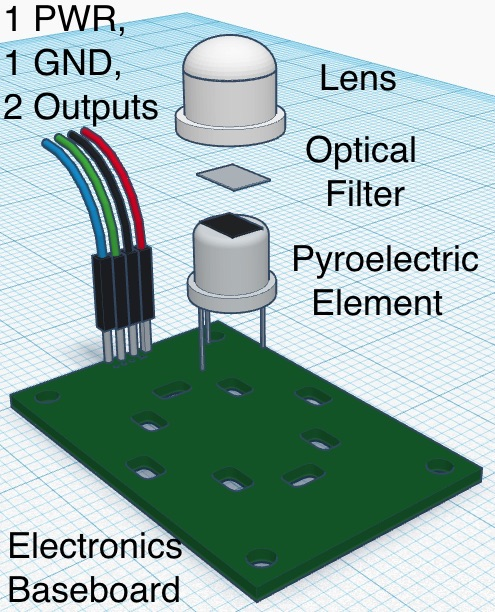
\includegraphics[width=0.2\textwidth, height=1.3in]{figures/platform/3d_view_5-annotated.jpg}
        \caption{PIR Sensor Teardown showing the different subsystems illustrated in TinkerCAD}
        \label{fig:pir_system_teardown}
    %\end{subfigure}%
    % \begin{subfigure}[b]{0.35\textwidth} %\scalebox{0.8}{}
    %     \begin{flushleft}
    %         %\centering
    %         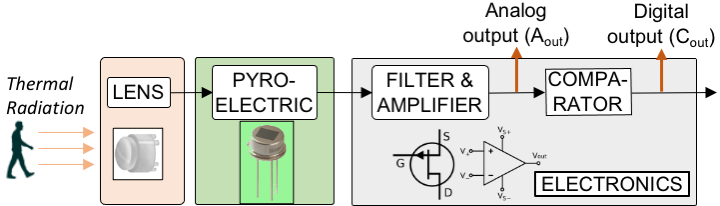
\includegraphics[width=1.2\textwidth]{figures/platform/pir-block-diagram-2-redraw-camera.png}
    %         \caption{}
    %         \label{fig:pir_working}
    %     \end{flushleft}
    % \end{subfigure}%
    %\hfill
    % \begin{subfigure}[b]{0.30\textwidth}
    %     \begin{flushright}
    %     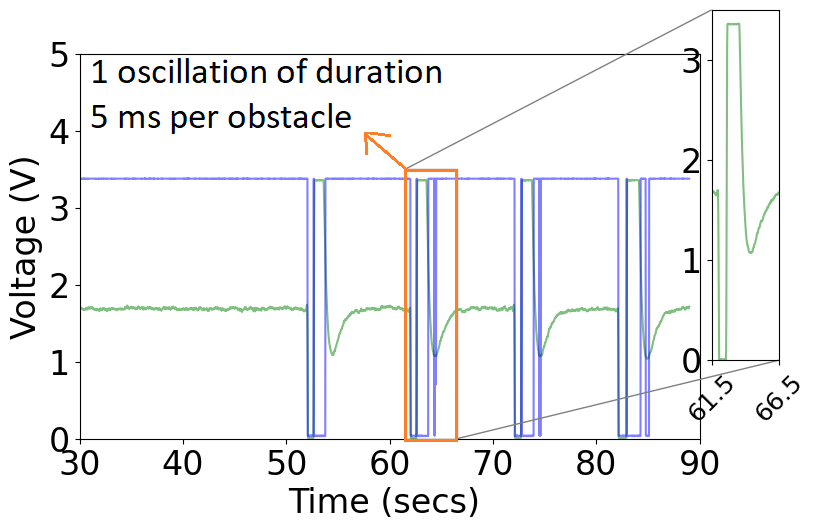
\includegraphics[width=0.9\textwidth]{figures/lens_types/inline_lens.png}
    %     \caption{}
    %     \label{fig:pir_output}
    %     \end{flushright}
    % \end{subfigure}%
    %\caption{\ca \hl{PIR Sensor Teardown}, \cb Internal components of a PIR sensor, \cc Output signals \aout (Green) and \cout (Blue) during sensor operation. \aout, (magnified) shows oscillations when an obstacle is detected}
%\end{figure} 
\end{wrapfigure}

\section{PIR Sensors}
\label{sec:approach}
We take a deep dive into a PIR sensor with 3 goals -- \ca understanding the physics of sensing (\S\ref{subsec:physics}, \S\ref{subsec:working}), \cb correlating physics to the failure scenarios (\S\ref{subsec:taxonomy}) and \cc analyzing the effect of these failures on the sensing performance (\S\ref{subsec:quantify}).

%% BEGINNING OUTLINE
% \begin{itemize}
%     \item Working of the PIR sensor
%     \item Warm behavior - Ashish will email Akshay warmup slides
%     \item Possible faults in PIR sensors - empirical experiments and understanding
%     \item How does $A_{out}$, $C_{out}$ look like for failed scenarios? Plot time domain data and visually show how sensor failure affects $A_{out}$.
% \end{itemize}
%% END OF OUTLINE
%\label{subsec:physics}
%In this section, we briefly describe the working of a PIR sensor and then present the potential failure scenarios in PIR sensors.

\subsection{Background}
\label{subsec:physics}
The teardown of a PIR sensor, showing the internal components is shown in {\bfseries Fig.~\ref{fig:pir_system_teardown}}.
%
%A PIR sensor internally comprises of 3 subsystems as shown in {\bfseries Fig.\ref{fig:pir_working}}  -- \ca a lens, \cb a pyroelectric, and \cc an electronic subsystem. These subsystems act in sequence \ie Lens $\rightarrow$ Pyroelectric $\rightarrow$ Electronic to perform the end-to-end sensing process as we describe next.
It comprises 3 subsystems -- \ca a lens, \cb a pyroelectric attached to an optical filter, and \cc an electronic subsystem.
%
These subsystems act in sequence \ie Lens $\rightarrow$ Pyroelectric $\rightarrow$ Electronic to perform the end-to-end sensing process as shown in {\bfseries Fig.~\ref{fig:pir_sensing_pipeline}}. We describe the different subsystems next.
%

\noindent \underline{\bfseries Lens Subsystem} A plastic fresnel lens~\cite{an_murata} is used to capture and precisely focus thermal radiation into an optical filter that is aimed at a pyroelectric element. 
%The lens is glued to the electronic board via an adhesive and is geometrically constructed to precisely focus thermal radiation on the pyroelectric element. 
Fresnel lenses have a large capture area (aperture) and are used to concentrate radiation into a narrow beam. % and provide a short focal length.
%
They are used to divide the entire region observable to the PIR sensor into small cells, which increases range of the sensor by manifolds. 
%
They have a large capture area (aperture) and are common in a wide variety of applications such as lighthouses, solar cells and even in optical landing systems in aircrafts~\cite{webster1999measurement}.


% \begin{figure*}
% 	%%%%%%%%%%%%%%%%
% 	% PIR SENSOR PIPELINE
% 	%%%%%%%%%%%%%%%%
% 	%\begin{subfigure}{0.48\textwidth}
% 	\begin{minipage}[b]{0.56\linewidth}
% 		%\begin{flushright}
% 		\centering
% 			\begin{subfigure}[t]{\textwidth}
% 				\includegraphics[width=\textwidth,height=0.9in]{figures/platform/pir-block-diagram-2.png}
% 				\caption{}
% 				\label{fig:pir_sensor_pipeline}
% 			\end{subfigure}\\
% 			\begin{subfigure}[t]{\textwidth}
% 				\includegraphics[width=\textwidth,height=0.7in]{figures/platform/sensys_workflow.png}
% 				\caption{}
% 				\label{fig:system_workflow}
% 			\end{subfigure}
% 		%\end{flushright}
% 		\caption{\ca \textbf{Physics of the} PIR Sensing Pipeline, \cb \textbf{End-to-end workflow} of \sol for fault detection and diagnosis.}
% 		\label{fig:pir_sensing_pipeline}
% 	\end{minipage}
% 	%\end{subfigure}%
% 	%%%%%%%%%%%%%%%%
% 	% END OF PIR SENSOR PIPELINE
% 	%%%%%%%%%%%%%%%%
% 	\hspace{5ex}
%     %%%%%%%%%%%%%%%%
%     % PIR Working
%     %%%%%%%%%%%%%%%%
% 	\begin{minipage}[b]{0.39\linewidth}
% 		\centering
% 		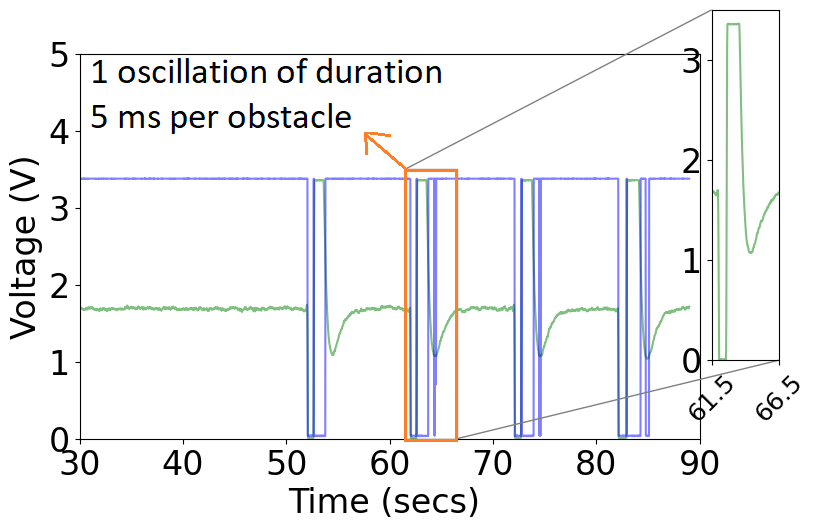
\includegraphics[width=\textwidth]{figures/lens_types/inline_lens.png}
% 		\caption{\textbf{Output signals \aout (Green) and \cout (Blue)} during sensor operation. \aout, (magnified) shows oscillations when an obstacle is detected.}
% 		\label{fig:pir_sensor_working}
% 	\end{minipage}
% 	%%%%%%%%%%%%%%%%
%     % END OF PIR Working
%     %%%%%%%%%%%%%%%%
% \end{figure*}

% Removing PIR Sensor Internals Figure
% \begin{figure*}%{htbp}
% 	%\begin{wrapfigure}{L}{9.5cm}
% 	% \centering
% 	%\vspace{-10pt}
% 	\begin{subfigure}[t]{0.5\textwidth}
% 		\centering
%     	\includegraphics[width=\textwidth]{figures/platform/pir-sensor-internals-2.png}%
%     	\caption{%\st{\textbf{Overview of PIR Sensor Internals} showing various subsystems.}
%     	}
%     	\label{fig:pir_sensor_overview}
% 	\end{subfigure}
% 	%\vspace{-10pt}
% 	%\end{wrapfigure}
% 	\hspace{5ex}
%     %%%%%%%%%%%%%%%%
%     % PIR Working
%     %%%%%%%%%%%%%%%%
% 	\begin{subfigure}[t]{0.4\textwidth}
% 		\centering
% 		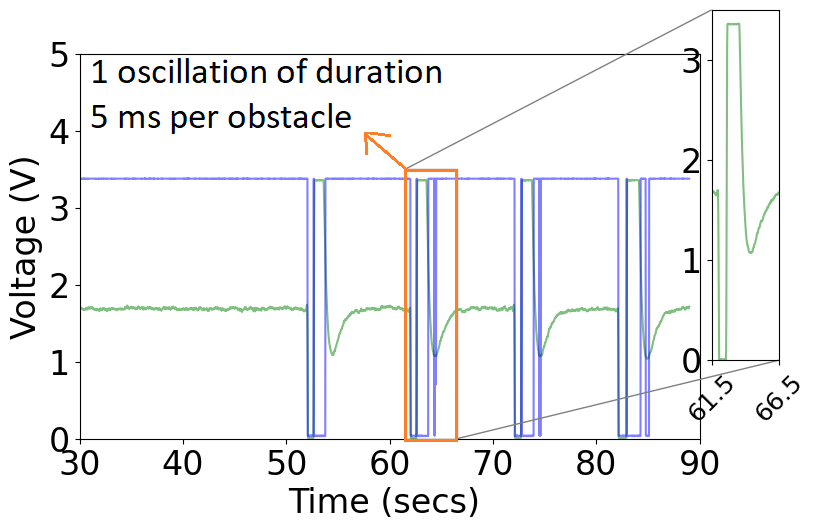
\includegraphics[width=\textwidth]{figures/lens_types/inline_lens.png}
% 		\caption{}
% 		\label{fig:pir_sensor_working}
% 	\end{subfigure}
% 	%%%%%%%%%%%%%%%%
%     % END OF PIR Working
%     %%%%%%%%%%%%%%%%
%     \caption{\ca \textbf{Close-up} of a COTS PIR sensor with its subsystems. \cb \textbf{Output signals \aout (Green) and \cout (Blue)} during sensor operation. \aout, (magnified) shows oscillations when an obstacle is detected.}
% \end{figure*}

\noindent \underline{\bfseries Pyroelectric Subsystem} comprises of an optical filter and a pair of pyroelectric elements. The optical filter is designed to filter out thermal radiations from wavelengths outside the human range (i.e., ~ 5 $\mu$m to 10 $\mu$m), which is then incident on the pyroelectric elements. % ({\bfseries Fig.\ref{fig:pir_system_teardown}}).
The pyroelectric elements convert the thermal radiation into an electrical voltage signal, a process known as the \textit{pyroelectric effect}. The output of the pyroelectric subsystem is an analog signal that is sent to the electronic subsystem.
In practice, there are two pyroelectric elements connected in series in a differential configuration. This differential configuration enables the PIR sensor to detect \textit{movement} of objects as static objects will trigger both the pyroelectric elements equally and cancel out unlike moving objects that trigger both elements unequally resulting in an output from the pyroelectric subsystem. %In other words, with the two pyroelectric elements opposing each other in the sensor, we get a differential voltage at the output of their combination. 
Due to the differential output voltage, the pyroelectric subsystem does not measure the absolute intensity of incident thermal radiation but measures a change in incident thermal radiation, say caused by motion. Note that the pyroelectric element by itself is passive \ie has no power source.

%That is, it produces a potential difference at its two terminals proportional to the incident light.
%This ensures that factors such as ambient room temperature have very less effect on the operation of the sensor.

\noindent \underline{\bfseries Electronic Subsystem} consists of a filter (RC filter), amplifier (JFET or OpAmp) and comparator (OpAmp) circuits. The output from pyroelectric subsystem are filtered to remove noise, amplified to increase its magnitude and finally sent to a comparator to convert analog signals to discrete signals. This \textit{discrete signal is HIGH when there is no motion and goes HIGH$\rightarrow$LOW when motion is detected}. Systems connected to a PIR sensor such as lighting or heating use the discrete signal to regulate the illumination or temperature in a building.

%%%%%%%%%%%%%%%%
% PIR Working
%%%%%%%%%%%%%%%%
% \begin{wrapfigure}{L}{7cm}
% 	% \begin{minipage}[t]{0.49\textwidth}
% 	\centering
% 	%\includegraphics[width=\textwidth, height=1.75in]{figures/pir/working/PIR_EVM_Charac_WithWithoutObstacle-2.png}
% 	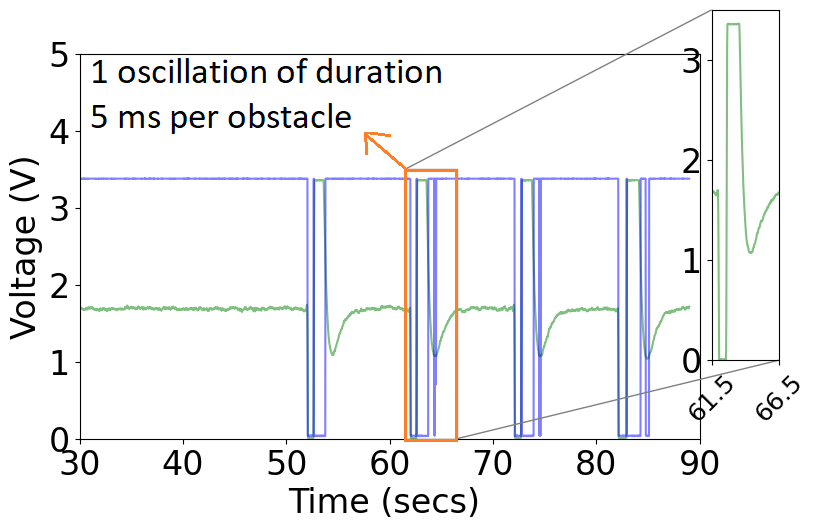
\includegraphics[width=6.5cm]{figures/lens_types/inline_lens.png}
% 	\caption{\textbf{Output signals \aout (Green) and \cout (Blue)} during sensor operation. \aout, drawn magnified shows the oscillations when an obstacle is detected.}
% 	\label{fig:pir_sensor_working}
% 	% \end{minipage}
% \end{wrapfigure}
%%%%%%%%%%%%%%%%
% END OF PIR Working
%%%%%%%%%%%%%%%%

%\subsection{Output Signals of a PIR Sensor}%The final output of the sensor is a discrete voltage signal, referred to as \cout that follows negative logic \ie stays HIGH when there is no motion and goes LOW when motion is detected. 

%The signal from the electronic system before sending it to the comparator is a filtered, amplified version of the output of the output of the pyroelectric subsystem -- this is called \aout.
% The differential voltage is then fed to the gate of a Junction Field-Effect Transistor (JFET). When the JFET is powered, the output at the source of the JFET is controlled by the output of the pyroelectric elements. The construction of the pyroelectric sensor is as shown in Figure. The pyroelectric elements and the JFET are encased in a housing and a filter is placed on top of the pyroelectric elements. This filter allows only infrared light to pass through. A fresnel lens is used to divide the entire region observable to the pyroelectric sensor into small cells. This increases the range of the sensor by manifolds.
% We will now present the working and physics of the PIR sensor.

%\begin{wrapfigure}{L}{0.7\textwidth}
\begin{figure}
	\centering
    \begin{subfigure}[b]{0.4\textwidth} %\scalebox{0.8}{}
        \begin{flushleft}
            %\centering
            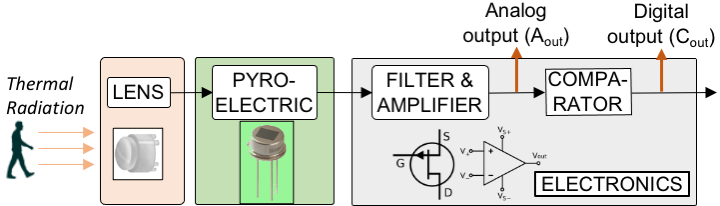
\includegraphics[width=\textwidth]{figures/platform/pir-block-diagram-2-redraw-camera.png}
            \caption{Sensing Pipeline of a PIR Sensor}
            \label{fig:pir_sensing_pipeline}
        \end{flushleft}
    \end{subfigure}%
    \hfill
	\begin{subfigure}[t]{0.3\textwidth}
		\centering
		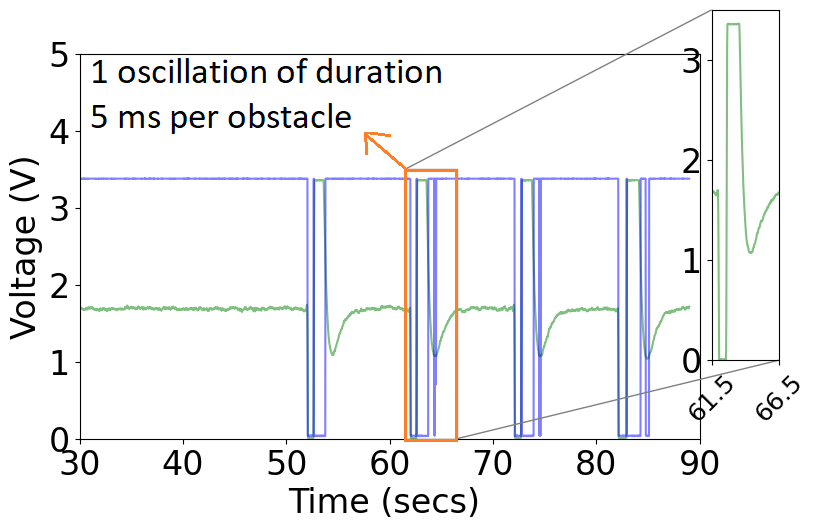
\includegraphics[width=\textwidth]{figures/lens_types/inline_lens.png}
		\caption{Inline lens (wall-mount)}
		\label{fig:inline_lens}
	\end{subfigure}%
    %\hspace{1ex}
	\begin{subfigure}[t]{0.3\textwidth}
		\centering
		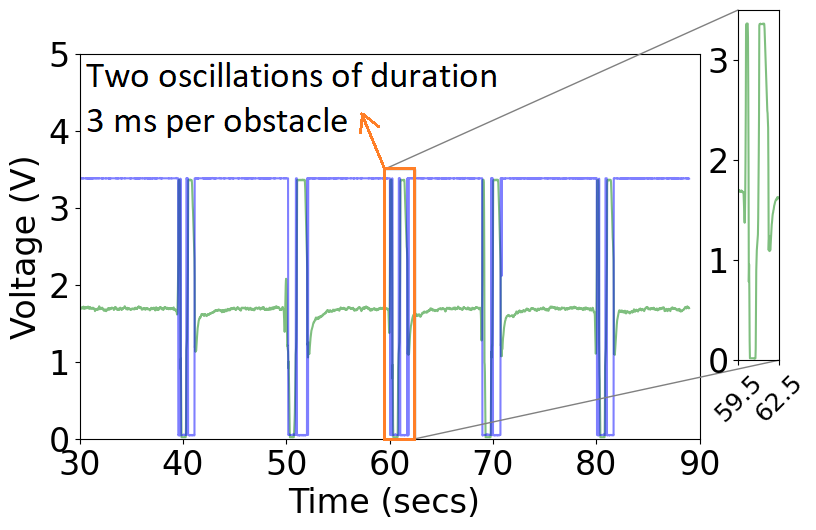
\includegraphics[width=\textwidth]{figures/lens_types/round_lens.png}
		\caption{Round lens (ceiling-mount)}
		\label{fig:round_lens}
	\end{subfigure}	   
	\caption{Effect of different types of lens on the \aout curve, shown in green -- the inline lens type produces a single oscillation whereas a round lens type produces two oscillation per obstacle. The corresponding \cout, shown in blue, stays HIGH when there is no motion and goes LOW when motion is detected. }
	\label{fig:pir_sensor_different_lens}
\end{figure}
%\end{wrapfigure}

\subsection{\textbf{Analysis of Output Signals of a PIR Sensor:}}
\label{subsec:working} 
There are 2 output signals from a PIR sensor as shown in {\bfseries Fig.~\ref{fig:pir_sensing_pipeline}}:
% \vspace{-5pt}
\begin{enumerate} \item \textbf{Final discrete output} of the electronic subsystem (\cout) that follows negative logic \ie stays HIGH when there is no motion and goes LOW when motion is detected. \item \textbf{Intermediate analog output} just prior to the discretization process (\aout). \end{enumerate}

%We consider the 2 output signals of the sensor -- \ci The Output from the Electronics (\cout) and \cii The Output from the Pyroelectric Element (\aout).  
To analyze \cout and \aout during operation, we interface a PIR sensor to an Arduino microcontroller~\cite{arduino_mega}. 
% This is plotted in \textbf{Fig.~\ref{fig:pir_sensor_working}} for a period of 60 seconds.
{\bfseries Fig.~\ref{fig:inline_lens} --~\ref{fig:round_lens}} shows plots of \aout and \cout for a period of 60 seconds, both in the presence and absence of an obstacle. The y-axis represents voltages seen at the output and x-axis represents time. As expected, %the discrete signal 
\cout, marked in blue, goes LOW when an obstacle comes into the field of view %(\ie there is motion) 
and stays HIGH otherwise. On the other hand, %the analog signal 
\aout, marked in green, measures around 1.8 V when there is no obstacle and produces oscillation(s) when an obstacle comes into the field of view (shown magnified). 
%
The nature and shape of the \aout curve also depends on the nature of lens used in the PIR sensor. Typically, an inline lens is used for the wall-mount version and a round lens is used for the ceiling-mount version. {\bfseries Fig.~\ref{fig:pir_sensor_different_lens}} also shows the variations in \aout between the two lens types -- \ca Inline lens has a wider curve compared to round lens and \cb Round lens has double number of oscillations of \aout curve per obstacle. We used a wall-mount PIR sensor in our experiments though our analysis, techniques and observations are equally applicable to ceiling-mount sensors. %sensing performance. 
%
With a working background on PIR sensors, we next study the various failures in a PIR sensor and its impact on sensing physics.
%\section{Background}

% \subsection{Overview of Sensor Types}  
% Sensors can be classified depending on the nature of its output data. 

% \noindent \textbf{Analog Sensors.} Analog sensors %, typically consisting of R, L and C elements, operate on the basis of transfer function to 
% provide an output value, which is continuous-valued. These sensors are noisy and require fine calibration but nevertheless are used due to its simplicity of operation and low cost. While faults in analog sensors are common, recently there have been approaches such as \cite{chakraborty2018fall} which aim at detecting performing fault isolation and detection for such sensors.

% \noindent \textbf{Digital \& Intelligent Sensors.} Digital sensors, on the other hand, provide a binary or discrete representation using an in-built analog-to-digital converter (ADC) \cite{webster_1999}. The key advantage digital sensors provides over analog sensors is the resistance to noise, lesser cabling complexity and ease of analysing and storing the sensor values \cite{analog_digital}. Typically, they use SPI or I2C interfaces and some digital sensors (we refer to them as \textit{intelligent} sensors) come with a light-weight processor that does some pre-processing and filtering of the raw sensor data to achieve such as data denoising. Intelligent sensors typically run proprietary vendor firmware that makes research difficult unless one has a contract with a vendor. Finally, economically, analog sensors are the cheapest while intelligent sensors are the most expensive whereas digital sensors occupy middle-ground. 

% \noindent \textbf{Faults.} Despite being more robust to noise than analog sensors and being equipped with pre-processing components to achieve better signal fidelity, there is little intrinsic support when one or more components fail in a digital sensor. This leads to unpredictable behavior ranging from \textit{false data}, \textit{stuck-at faults} to \textit{no data}. \Eg, a damaged (perhaps due to short circuit or even physical damage to the sensor)  soil moisture sensor can give false alarms or false assurances regarding soil moisture. Currently, one employs techniques such as spatial redundancy by sensor duplication or periodic manual calibration against a known, functional sensor to guard against sensor failure. In addition, these techniques do not identify the root \textit{cause} of the failure - whether it was the on-electronics that degraded or if it is due to failure of the sensing subsystem. Today, there are many industries such as manufacturing systems \cite{potok2018sdcworks}, agriculture \cite{patil2016model}, smart cities \cite{arasteh2016iot} that rely on digital sensors for its core operations and rely on proper functioning of sensors for providing real-time analytics and enhancing operating efficiency.  

% We look at Passive Infra-Red (PIR) sensors and Mass Air Flow (MAF) sensors which are two canonical examples of digital sensors. For the remainder of this section, we look at understanding the \textit{operational physics}  of these sensors, and leverage this to gain a \textit{subsystems view} of the sensor. This will enable us to systematically develop a taxonomy of failures in these sensors. 

%\subsection{Passive Infra-Red (PIR) Sensors}

% Passive Infra-Red (PIR) sensors are the predominant class of commodity human occupancy sensors used in buildings and industries for applications such as security alarms and electric lighting. The raw data from a PIR sensor is a binary output which indicates presence (LOW) or absence (HIGH) of a human object. PIR sensors are also used for composite applications beyond detection \eg Narayana \etal uses an array of PIR sensors to characterize the dimension of a human object and also perform localization within a space \cite{narayana2015pir}. 

% These sensors consist of a front face of an arrangement of optics (\viz fresnel lens and mirrors) feeding light into a pyroelectric element housed in an insulated casing connected to electronics aiding interfacing to other components in the IoT subsystem. Commonly available PIR sensors come in 2 form factors - integrated modules (Fig. \ref{fig:pir_sensor_module}) and evaluation boards. Integrated modules are pre-configured for end-user installation whereas evaluation boards allow re-configurability by giving capability to change individual sensor components as well as give electrical points to tap into different signals in the sensor circuitry. 

% \begin{figure}
% \vspace*{-1\baselineskip}
% \centering
% \includegraphics[scale=0.25]{figures/pir/pictures/pir-sensor-module.png}
% %\vspace*{-1.0\baselineskip}
% \caption{A commodity PIR sensor consisting of a plastic Fresnel lens cap focusing invisible infrared rays into a pyroelectric element beneath the cap. The sensor comes with supporting electronics to amplify, denoise and process the output from the pyroelectric element}
% \vspace*{-1\baselineskip}
% \label{fig:pir_sensor_module}
% \end{figure}

% \begin{figure}
% \centering
% \includegraphics[width=2.5in]{figures/pir/pictures/pir-sensor-evaluation-kit.jpg}
% %\vspace*{-1.0\baselineskip}
% \caption{PIR sensor evaluation kit to fingerprint the sensors in hardware}
% \vspace*{-1\baselineskip}
% \label{fig:pir_sensor_evm}
% \end{figure}

\textit{Type of Sensor} PIR is a passive sensor, which means that the sensing element does not consume power externally. 

\subsubsection{Warm-up Behavior} \ashish{@Sumukh - could you fill this in? You can refer to Figure 17 and 18 at the end of this paper which you had collected}

\subsection{Failure Signature} Recall above that the PIR sensors have 2 critical signals \viz $C_{out}$ and $A_{out}$ with $C_{out}$ being a discretized representation of the analog signal $A_{out}$. We characterize both of these signals to develop a \textit{failure signature} of the PIR sensor that can be used for classifying and identifying faults. We argue that the $A_{out}$ signal - \ca contains information characterizing the sensor and \cb can be used to detect and identify failures. These signals are used, in combination, because of two desirable characteristics:
\begin{itemize}
    \item \textit{Independent of Environment} \ashish{correction reqd.}
    \item \textit{Unique}
\end{itemize}

Examples of $A_{out}$ are shown in Figure~\ref{fig:pir_sensor_evm}-Figure~\ref{fig:msr_cafeteria}. We characterize the harmonic oscillations in $A_{out}$ to determine the \textit{working status} of different subsystems in the sensor.  We perform this using a frequency domain representation of the $A_{out}$ signal using Fast fourier transform coefficients and its variant power spectral density. 

% \begin{figure*}
% 	\centering
% 	\subfloat[\label{}]{%
% 		\includegraphics[width=0.32\linewidth]{figures/pir/working/signature/cafeteria/cafeteria-FFTAou.png}}
% 	\subfloat[\label{}]{%
% 		\includegraphics[width=0.32\linewidth]{figures/pir/working/signature/sensor1/working_data_run4_formatted-FFTAou.png}}
% 	\subfloat[\label{}]{%
% 		\includegraphics[width=0.32\linewidth]{figures/pir/working/signature/sensor2/working_data_with_obstacle_run2_formatted-FFTAou.png}}\\
% 	\subfloat[\label{}]{%
% 		\includegraphics[width=0.32\linewidth]{figures/pir/working/signature/sensor3/PIR_EVM_Charac_WithObstacle-FFTAou.png}}
% 	\subfloat[\label{}]{%
% 		\includegraphics[width=0.32\linewidth]{figures/pir/working/signature/sensor4/pir_evm_raw_data-FFTAou.png}}
% 	\subfloat[\label{}]{%
% 		\includegraphics[width=0.32\linewidth]{figures/pir/working/signature/slow_obstacle/slow_obstacle-FFTAou.png}}
% 	\caption{Failure signature in 6 fully function sensors captured in different environment show presence of the frequencies between 0-5Hz and negligible outside that}
% 	\label{fig:signature}
% \end{figure*}


\subsubsection{Type of lens} The pattern of $A_{out}$ upon obstacle detection depends on the type of lens installed - \ca inline lens (Fig~\ref{fig:pir_sensor_wall_mount}), or \cb round lens (Fig~\ref{fig:pir_sensor_ceiling_mount}). Typically, round lenses were used in PIR sensors deployed on ceilings and inline lenses in wall-mount PIR sensors. The sensors differ in 2 aspects - \begin{itemize} \item The duration of the $A_{out}$ pulse upon obstacle detection depend on the type of the lens \viz in case of inline lens, each pulse is of 5 ms (\ie slower) and in case of round lens, it is of 3 ms (\ie faster), \item The number of zero-crossings of $A_{out}$ in case of round lens is larger (\viz 5) in comparison with inline lens (\viz 3),
\item Return back to zero of the last oscillation is much slower for inline lens as compared to round lens.
\end{itemize}

\subsubsection{A note on speed of obstacle} The detection pulse on $A_{out}$ is dependent on the rate of coverage of the angular detection region. Therefore a very fast obstacle moved in front of the sensor would trigger rapid oscillations in the detection pulse. However, this does not affect our fault detection approach for 2 reasons - \ci We observe that the nature of $A_{out}$ is deterministic for naturally observed speeds in buildings such as a human walking or a hand waving (\eg Fig.~\ref{fig:msr_cafeteria}), and \cii Our goal is not to determine the size or speed of the object but to detect faults in the sensors. Additionally, we can perform the fault detection process over multiple time windows to filter out false positives. An example run with a fast-moving obstacle is as shown in Figure~\ref{fig:pir_sensor_fast_obstacle}. 

\begin{figure}
\centering
\includegraphics[scale =0.25]{figures/pir/working/FastObstacle/working_data_run3_formattedfast-obstacle.png}
\caption{$A_{out}$ when the obstacle is moving rapidly.}
\label{fig:pir_sensor_fast_obstacle}
\end{figure}

\begin{figure}
\centering
\includegraphics[scale =0.25]{figures/pir/working/MSRCafeteria/cafeteriacafeteria-withoutinset.png}
\caption{$A_{out}$ in a practical deployment at a cafeteria in Bangalore showing the constituent frequencies present.}
\label{fig:msr_cafeteria}
\end{figure}





%%BEG OF COMMENT
\begin{table*}[htb]
  \centering
    \begin{tabular}{| p{2cm}| m{7cm} | m{7cm} | }
        \hline
        \bfseries Sensor Type & 
        \bfseries Time Domain &  
        \bfseries Frequency Domain Spectrum \\ \hline 
        
        \hline
        Working Sensor &         
        \begin{minipage}{.35\textwidth}
        \includegraphics[width=\linewidth]{figures/frequency/FreshCharacterization/Working/working_obstacle/Cout-Aout.png}
        \end{minipage} & 
        \begin{minipage}{.35\textwidth}
        \includegraphics[width=\linewidth]{figures/frequency/FreshCharacterization/Working/working_obstacle/Spectrogram.png}
        \end{minipage} \\ 
        
        \hline
        Class I Faulty (Lens Dislodged ~ 45$^{\circ}$) &         
        \begin{minipage}{.35\textwidth}
        \includegraphics[width=\linewidth]{figures/frequency/FreshCharacterization/ClassI/lensdislodged_obstacle/Cout-Aout.png}
        \end{minipage} & 
        \begin{minipage}{.35\textwidth}
        \includegraphics[width=\linewidth]{figures/frequency/FreshCharacterization/ClassI/lensdislodged_obstacle/Spectrogram.png}
        \end{minipage} \\ 

        \hline
        Class I Faulty (Lens off) &         
        \begin{minipage}{.35\textwidth}
        \includegraphics[width=\linewidth]{figures/frequency/FreshCharacterization/ClassI/lensoff_obstacle/Cout-Aout.png}
        \end{minipage} & 
        \begin{minipage}{.35\textwidth}
        \includegraphics[width=\linewidth]{figures/frequency/FreshCharacterization/ClassI/lensoff_obstacle/Spectrogram.png}
        \end{minipage} \\        
        
        \hline
        Class II Faulty (Lens Deformed) &         
        \begin{minipage}{.35\textwidth}
        \includegraphics[width=\linewidth]{figures/frequency/FreshCharacterization/ClassII/lensdeformed_obstacle/Cout-Aout.png}
        \end{minipage} & 
        \begin{minipage}{.35\textwidth}
        \includegraphics[width=\linewidth]{figures/frequency/FreshCharacterization/ClassII/lensdeformed_obstacle/Spectrogram.png}
        \end{minipage} \\            
        
        \hline
        Class II Faulty (Lens Puncture) &         
        \begin{minipage}{.35\textwidth}
        \includegraphics[width=\linewidth]{figures/frequency/FreshCharacterization/ClassII/lenspuncture_obstacle/Cout-Aout.png}
        \end{minipage} & 
        \begin{minipage}{.35\textwidth}
        \includegraphics[width=\linewidth]{figures/frequency/FreshCharacterization/ClassII/lenspuncture_obstacle/Spectrogram.png}
        \end{minipage} \\ 
        \hline
        
    \end{tabular}
  \caption{Basic Characterization of PIR Sensors}
  \label{tbl:basic_char}
\end{table*}


\begin{table*}[htb]
  \centering
    \begin{tabular}{| p{2cm}| m{7cm} | m{7cm} | }
        \hline
        \bfseries Sensor Type & 
        \bfseries Time Domain &  
        \bfseries Frequency Domain Spectrum \\ \hline 
        
        \hline
        Class III Faulty  (Dust) &         
        \begin{minipage}{.35\textwidth}
        \includegraphics[width=\linewidth]{figures/frequency/FreshCharacterization/ClassIII/dust_obstacle/Cout-Aout.png}
        \end{minipage} & 
        \begin{minipage}{.35\textwidth}
        \includegraphics[width=\linewidth]{figures/frequency/FreshCharacterization/ClassIII/dust_obstacle/Spectrogram.png}
        \end{minipage} \\
        
        \hline
        Class III Faulty  (Paper) &         
        \begin{minipage}{.35\textwidth}
        \includegraphics[width=\linewidth]{figures/frequency/FreshCharacterization/ClassIII/paper_obstacle/Cout-Aout.png}
        \end{minipage} & 
        \begin{minipage}{.35\textwidth}
        \includegraphics[width=\linewidth]{figures/frequency/FreshCharacterization/ClassIII/paper_obstacle/Spectrogram.png}
        \end{minipage} \\
        
        \hline
        Class IV Faulty  (Window Damage - Oil) &         
        \begin{minipage}{.35\textwidth}
        \includegraphics[width=\linewidth]{figures/frequency/FreshCharacterization/ClassIV/windowdamageoil_obstacle/Cout-Aout.png}
        \end{minipage} & 
        \begin{minipage}{.35\textwidth}
        \includegraphics[width=\linewidth]{figures/frequency/FreshCharacterization/ClassIV/windowdamageoil_obstacle/Spectrogram.png}
        \end{minipage} \\
        
        \hline
        Class V Faulty  (Electronic Fault) &         
        \begin{minipage}{.35\textwidth}
        \includegraphics[width=\linewidth]{figures/frequency/FreshCharacterization/ClassV/electronicfault_obstacle/Cout-Aout.png}
        \end{minipage} & 
        \begin{minipage}{.35\textwidth}
        \includegraphics[width=\linewidth]{figures/frequency/FreshCharacterization/ClassV/electronicfault_obstacle/Spectrogram.png}
        \end{minipage} \\
        \hline 
        

    \end{tabular}
  \caption{Basic Characterization of PIR Sensors (Contd)}
  \label{tbl:basic_char_contd}
\end{table*}

%%END OF COMMENT

% \begin{table*}[htb]
%   \centering
%     \begin{tabular}{| p{2cm}| m{7cm} | m{7cm} | }
%         \hline
%         \bfseries Sensor Type & 
%         \bfseries Time Domain &  
%         \bfseries Frequency Domain Spectrum \\ \hline 
        
%         \hline
%         Working Sensor &         
%         \begin{minipage}{.35\textwidth}
%         \includegraphics[width=\linewidth]{figures/frequency/FreshCharacterization/Working/working_obstacle/Cout-Aout.png}
%         \end{minipage} & 
%         \begin{minipage}{.35\textwidth}
%         \includegraphics[width=\linewidth]{figures/frequency/FreshCharacterization/Working/working_obstacle/Spectrogram.png}
%         \end{minipage} \\ 
        
%         \hline
%         Class I Faulty (Lens Dislodged ~ 45$^{\circ}$) &         
%         \begin{minipage}{.35\textwidth}
%         \includegraphics[width=\linewidth]{figures/frequency/FreshCharacterization/ClassI/lensdislodged_obstacle/Cout-Aout.png}
%         \end{minipage} & 
%         \begin{minipage}{.35\textwidth}
%         \includegraphics[width=\linewidth]{figures/frequency/FreshCharacterization/ClassI/lensdislodged_obstacle/Spectrogram.png}
%         \end{minipage} \\ 

%         \hline
%         Class I Faulty (Lens off) &         
%         \begin{minipage}{.35\textwidth}
%         \includegraphics[width=\linewidth]{figures/frequency/FreshCharacterization/ClassI/lensoff_obstacle/Cout-Aout.png}
%         \end{minipage} & 
%         \begin{minipage}{.35\textwidth}
%         \includegraphics[width=\linewidth]{figures/frequency/FreshCharacterization/ClassI/lensoff_obstacle/Spectrogram.png}
%         \end{minipage} \\        
        
%         \hline
%         Class II Faulty (Lens Deformed) &         
%         \begin{minipage}{.35\textwidth}
%         \includegraphics[width=\linewidth]{figures/frequency/FreshCharacterization/ClassII/lensdeformed_obstacle/Cout-Aout.png}
%         \end{minipage} & 
%         \begin{minipage}{.35\textwidth}
%         \includegraphics[width=\linewidth]{figures/frequency/FreshCharacterization/ClassII/lensdeformed_obstacle/Spectrogram.png}
%         \end{minipage} \\            
        
%         \hline
%         Class II Faulty (Lens Puncture) &         
%         \begin{minipage}{.35\textwidth}
%         \includegraphics[width=\linewidth]{figures/frequency/FreshCharacterization/ClassII/lenspuncture_obstacle/Cout-Aout.png}
%         \end{minipage} & 
%         \begin{minipage}{.35\textwidth}
%         \includegraphics[width=\linewidth]{figures/frequency/FreshCharacterization/ClassII/lenspuncture_obstacle/Spectrogram.png}
%         \end{minipage} \\ 
%         \hline
        
%     \end{tabular}
%   \caption{Basic Characterization of PIR Sensors}
%   \label{tbl:basic_char_contd_cont}
% \end{table*}


% \begin{table*}[htb]
%   \centering
%     \begin{tabular}{| p{2cm}| m{7cm} | m{7cm} | }
%         \hline
%         \bfseries Sensor Type & 
%         \bfseries Time Domain &  
%         \bfseries Frequency Domain Spectrum \\ \hline 
        
%         \hline
%         Class III Faulty  (Dust) &         
%         \begin{minipage}{.35\textwidth}
%         \includegraphics[width=\linewidth]{figures/frequency/FreshCharacterization/ClassIII/dust_obstacle/Cout-Aout.png}
%         \end{minipage} & 
%         \begin{minipage}{.35\textwidth}
%         \includegraphics[width=\linewidth]{figures/frequency/FreshCharacterization/ClassIII/dust_obstacle/Spectrogram.png}
%         \end{minipage} \\
        
%         \hline
%         Class III Faulty  (Paper) &         
%         \begin{minipage}{.35\textwidth}
%         \includegraphics[width=\linewidth]{figures/frequency/FreshCharacterization/ClassIII/paper_obstacle/Cout-Aout.png}
%         \end{minipage} & 
%         \begin{minipage}{.35\textwidth}
%         \includegraphics[width=\linewidth]{figures/frequency/FreshCharacterization/ClassIII/paper_obstacle/Spectrogram.png}
%         \end{minipage} \\
        
%         \hline
%         Class IV Faulty  (Window Damage - Oil) &         
%         \begin{minipage}{.35\textwidth}
%         \includegraphics[width=\linewidth]{figures/frequency/FreshCharacterization/ClassIV/windowdamageoil_obstacle/Cout-Aout.png}
%         \end{minipage} & 
%         \begin{minipage}{.35\textwidth}
%         \includegraphics[width=\linewidth]{figures/frequency/FreshCharacterization/ClassIV/windowdamageoil_obstacle/Spectrogram.png}
%         \end{minipage} \\
        
%         \hline
%         Class V Faulty  (Electronic Fault) &         
%         \begin{minipage}{.35\textwidth}
%         \includegraphics[width=\linewidth]{figures/frequency/FreshCharacterization/ClassV/electronicfault_obstacle/Cout-Aout.png}
%         \end{minipage} & 
%         \begin{minipage}{.35\textwidth}
%         \includegraphics[width=\linewidth]{figures/frequency/FreshCharacterization/ClassV/electronicfault_obstacle/Spectrogram.png}
%         \end{minipage} \\
%         \hline 
        

%     \end{tabular}
%   \caption{Basic Characterization of PIR Sensors (Contd)}
%   \label{tbl:basic_char_contd_contd_contd}
% \end{table*}

\subsection{Failures in PIR Sensors -- A Taxonomy} 
\label{subsec:taxonomy} 

%%%%%%%%%%%%%%%%
% FAILURE PHOTOGRAPHS
%%%%%%%%%%%%%%%%
\begin{figure}%[t]
	\centering
	\small
	\begin{subfigure}[t]{0.24\textwidth}
		\centering
		\includegraphics[width=\textwidth]{figures/platform/failure_photographs/WorkingSensor-proper.jpg}
		\caption{\footnotesize Working Sensor}
		\label{fig:working}
	\end{subfigure}
	\hspace{0.10ex}%
	\begin{subfigure}[t]{0.24\textwidth}
		\centering
		\includegraphics[width=\textwidth]{figures/platform/failure_photographs/ClassI-LensCapRemoved-annotated-jpg.jpg}
		\caption{Lens Cap Fallen Off}
		\label{fig:failure_photo1}
	\end{subfigure}
	\hspace{0.10ex}
	\begin{subfigure}[t]{0.24\textwidth}
		\centering
		\includegraphics[width=\textwidth]{figures/platform/failure_photographs/ClassI-LensCapDislogdged-annotated-jpg.jpg}
		\caption{\footnotesize Lens Cap Dislocated}
		\label{fig:failure_photo2}
	\end{subfigure}	
	\hspace{0.10ex}
	\begin{subfigure}[t]{0.24\textwidth}
		\centering
		\includegraphics[width=\textwidth]{figures/platform/failure_photographs/ClassII-LensCapDeformed-annotated-jpg.jpg}
		\caption{Lens Cap Deformed}
		\label{fig:failure_photo3}
	\end{subfigure}
	\begin{subfigure}[t]{0.24\textwidth}
		\centering
		\includegraphics[width=\textwidth]{figures/platform/failure_photographs/ClassII-LensCapPunctured_new-2-annotated.png}
		\caption{Lens Cap Punctured}
		\label{fig:failure_photo4}
	\end{subfigure}
	\hspace{0.1ex}
	\begin{subfigure}[t]{0.24\textwidth}
		\centering
		\includegraphics[width=\textwidth]{figures/platform/failure_photographs/ClassIII-LensCapCovered-annotated-jpg.jpg}
		\caption{\footnotesize Lens Cap Covered}
		\label{fig:failure_photo5}
	\end{subfigure}
	\hspace{0.1ex}%
	\begin{subfigure}[t]{0.24\textwidth}
		\centering
		\includegraphics[width=\textwidth]{figures/platform/failure_photographs/ClassIV-OpticalFilterDamage-annotated-jpg.jpg}
		\caption{\footnotesize Optical Filter Damaged}
		\label{fig:failure_photo6}
	\end{subfigure}	
	\hspace{0.1ex}
	\begin{subfigure}[t]{0.24\textwidth}
		\centering
		\includegraphics[width=\textwidth]{figures/platform/failure_photographs/ClassV-ElectronicsFault-annotated-jpg.jpg}
		\caption{Electronic Fault}
		\label{fig:failure_photo7}
	\end{subfigure}	
	%\vspace{-10pt}
	\caption{\footnotesize{Some sensors} used in our study. Note that the failures are not always visually perceivable as the sensors are typically inaccessible.}
	\label{fig:pir_sensor_failure_photographs}
	%\vspace{-5pt}
\end{figure}

%%%%%%%%%%%%%%%%
% END OF FAILURE PHOTOGRAPHS
%%%%%%%%%%%%%%%%



%A PIR sensor can fail in multiple ways. Irrespective of the nature of failures, all failures lead to a compromised operation of the sensor resulting in data that is incorrect and lacking fidelity. 
Fundamentally, failures in a PIR sensor could occur either on the lens, the pyroelectric element or the electronics. We \textit{analyze and categorize practical, common and most frequent} failures as gathered in discussions with IoT engineers and technicians who install and maintain PIR sensor deployments. 
% We talked to technicians at our university building in the US as well as at our office building in India.
% Consequently, uncommon failures such as those due to cosmic rays and alpha-particles are outside the scope of this discussion. 
% Nevertheless, if the designer needs to account for esoteric failures, our framework provides a guideline for analysis.
%We next describe these common failures in each subsystem and study them in detail. 
We developed a new taxonomy for such failures, as summarized in {\bfseries Table~\ref{tab:pir_faults}} and visualized in {\bfseries Fig.~\ref{fig:pir_sensor_failure_photographs}}. 
% Note that failures are not necessarily binary in nature \ie there can be partial or temporary failures (degradation).

%\begin{table}%[b]
\begin{wraptable}{R}{0.65\textwidth}%[ht]\small
%\renewcommand{\arraystretch}{1.1}
%\vspace{-\baselineskip}
	\centering
	\footnotesize
    \caption{{\bfseries Taxonomy of Failures} in a PIR Sensor}
    \begin{tabular}{p{2.25cm} p{6cm}}
    \hline %\\
    \textsc{\bfseries Failure} & \textsc{\bfseries Definition \& Impact}\\
    \hline\hline
    \rowcolor{gray!20} \multicolumn{2}{l}{\bfseries Lens Subsystem}\\
    Lens dislodged \newline (Class I) & Lens cap suffers partial or complete dislocation \eg physical impact with a foreign object, degradation of bonding,~\etc \\
    Lens deformed \newline (Class II) & Lens cap suffers physical damage in-place \eg deformation, puncture,~\etc \\
    Lens covered \newline (Class III) & Lens cap gets physically obstructed by foreign particles \eg dust, paper or tape \\
    \hline
    \rowcolor{gray!20} \multicolumn{2}{l}{\bfseries Pyroelectric Subsystem} \\
    Optical filter \newline damage (Class IV) & Damaged by environmental factors~\eg oil condensation\\
    \hline
    \rowcolor{gray!20} \multicolumn{2}{l}{\bfseries Electronic Subsystem} \\
    Electronic faults \newline (Class V) & Hardware failures~\eg short circuits, floating outputs~\etc \\
    % Thermal Faults & Pyroelectric element can degrade or age and can give imperfect output\\
    \hline
    \end{tabular}
    \label{tab:pir_faults}
    %\vspace{-15pt}
    %\vspace{-\baselineskip}
\end{wraptable}
%\end{table}

\subsubsection{\textbf{Failures in the lens subsystem}} The lens is geometrically constructed to precisely focus the thermal rays onto the pyroelectric element. As a result, failures affecting the optical integrity of the lens can result in loss of precision for focusing the thermal rays. We observe three types of failures here, termed Class I--III failures.

\noindent \underline{Lens dislocation (Class I):} %Generally, the lens is either stuck onto the sensor board with an adhesive material or is constructed with hooks that latch onto the the sensor board (refer Fig. \ref{fig:pir_sensor_overview}). Thus, as a result of this, in deployment, 
As the lens is stuck on the sensor board with an adhesive or machined to fit over the pyroelectric element, it could get dislodged from its place or completely fall off the sensor board due to factors such as thermal expansion or physical impact. 
% We name these Class I failures.
%The result is loss of focus of thermal radiation on the pyroelectric element. 

\noindent \underline{Lens deformation (Class II):} As the lens is made of flexible, 0.4mm thick high density plastic~\cite{fresnel}, it is susceptible to deformation by physical damage. This can alter the curvature or puncture the lens. %We term such failures as Class II failures. 
%
As in Class I, the consequence of failure is imperfect capture and focusing of the thermal radiation incident on the PIR sensor.
%

\noindent \underline{Lens hindrance (Class III):} Dust particles (\eg factory floors, building construction) or common objects such as paper and plastic tape can absorb the thermal radiation resulting in reduced to no radiation falling on the pyroelectric element. The deposition of particulate matter also causes dispersion.
%These are termed Class III failures.% We refer to these as Class III failures.

In summary, Classes I--III failures affect the core functionality of the lens, and results in the imperfect capture and focus of thermal radiation.
%results in the imperfect capture and focus of thermal radiation thus affecting the core functionality of the lens.
% resulting in change in the ability of the lens to focus the narrow beam. 

\subsubsection{\textbf{Failures in the pyroelectric subsystem}: Optical Filter Damage (Class IV):} %The pyroelectric subsystem is another critical point of failure in a PIR sensor.  
The optical filter and pyroelectric elements are prone to degradation with exposure to high temperature and humidity. As the optical filter is carefully calibrated to trigger in the region of human motion, it is susceptible to damage due to environmental factors such as heat sources (\eg room heaters, air-conditioners) and humidity (\eg oil condensation) as it affects the perceived temperature of the object. We name these as Class IV failures.

\subsubsection{\textbf{Failures in the Electronics}} On-board electronics consisting of filter, amplifier and comparator circuitry are prone to failures such as shorted or floating pins that we refer to as Class V failures. We only consider simple, electronic failures -- such as open, short circuits and floating inputs. Vendor-based IC testing procedures and board design process advancements have made electronic failures such as regulator, bus failures and PCB malfunctions infrequent in practice.
%, and degradation due to elements such as temperature and humidity. 

%\noindent \textbf{Note:} In this study, we
%\st{do not consider hardware electronic failures such as PCB malfunctions and} 
%only consider simple electronics failures -- vendor-based IC testing procedures during board design process advancements have made electronics failures such as regulator failures, bus failures and PCB malfunctions infrequent.% one part per billion~\cite{}. 

%Instead, our focus is squarely on practical failures, and damage that can occur from the environment during deployment. We gathered these in discussion with PIR sensor manufacturers and smart building deployment technicians at our LEED-certified building. Lastly, we do not consider ageing of the PIR sensor separately as a fault. It is subsumed in the other failure scenarios.

\noindent \textbf{Summary:} Failures in PIR sensors can occur in either the lens subsystem, the pyroelectric subsystem or the on-board electronics, each of which manifest differently in the underlying physics.
%Each of these failures manifest differently in the underlying physics.% of sensing and thereby impact the sensor operation differently.


\subsection{Analyzing Severity of Failures -- A Quantitative Analysis}
\label{subsec:quantify}
A failure is said to impact the sensor performance if the failure results in either false detections ({\bfseries FD}) \ie false positives or missed obstacles ({\bfseries MO}) \ie false negatives in the sensor output (\cout), compared to a working sensor. As seen in {\bfseries Fig.~\ref{fig:pir_sensor_different_lens}}, \cout is HIGH (1) when no is obstacle detected and \cout goes HIGH (1) $\rightarrow$ LOW (0) when an obstacle is detected.

%To investigate the manner in which failure can affect the reliability of the PIR sensor, we investigate the output of the sensor \ie \cout. 

\noindent \underline{Controlled Failure Study:} To understand the impact on sensor performance, in our lab, we take 2 PIR sensors, one which is without the fault (\working) and one with the fault (\tampered). The 2 sensors are placed in as close a proximity to one another as possible such that -- \ca distance between the sensors are closer than the size of obstacle, \cb the obstacle is moved in a plane such that it comes into the detection region of both the PIR sensors simultaneously. This implies that when the obstacle (we used our palm in this case) is moved across the detection region of both PIR sensors, it grazed both at the same time, triggering the same responses from both the sensors.

We then calculate the absolute difference ($\delta_N$) between the \cout values of the tampered sensor~\viz  \couttampered and the reference working sensor~\viz \coutworking by summing over all observations (Refer Eqn.~\ref{eqn:1}). Intuitively, a relatively low $\delta_N$ would imply that the tampered sensor is still in acceptable condition \ie the failure is not having much impact on the operation of the sensor. On the other hand, a high value of difference implies that the failure is much serious. To ease computation, we can also compute $\delta_N$ by dividing the time series into equal size chunks called \textit{windows} (W) and computing the difference between average \cout values of \tampered and \working in that window.

\begin{table}%[b]
	\small
	\centering
	\caption{\textbf{Misclassifications} analysis for different failures. The numbers indicate the deviation (as defined in Eqn.~\ref{eqn:1} between $C_{out}$ values) of a faulty sensor from that of a working sensor. Higher number indicates increased degree of failure.}
	%\begin{tabular}{lcccc}
	\begin{tabular}{lllll}
		%\begin{tabular}{p{2cm}p{2cm}p{2cm}p{2cm}p{2cm}}
		\hline
		\bfseries \textsc{Failure} & \bfseries \textsc{Lens Dislodged} & \bfseries \textsc{Lens Covered} & \bfseries \textsc{Heat Damage} & \bfseries \textsc{Humidity Damage}\\
		\hline \hline
		\rowcolor{gray!20} $\delta_N$$^1$ & 35 & 48 & 29 & 48 \\
		$\delta_N$$^2$ & 69 & 94  & 53 & 87 \\
		\hline 
	\end{tabular}
	\label{tbl:fault_degree}
	%\vskip1pt
	\quad \raggedright
	$^1$ 6 hour run, $^2$ 12 hour run
\end{table} 

\textbf{Table~\ref{tbl:fault_degree}} summarizes $\delta_N$ for a few types of failures as observed over 6-hour and 12-hour runs deployed in the elevator of our building. The numbers in the column represent deviation or misclassifications ($\delta_N$)~\ie the number of false detections (both false positives and false negatives) by the faulty sensor calculated using {\bfseries Eqn.~\ref{eqn:1}}.
%In long deployments, 
We used a window size, $W$ = 1024 samples, which comes to a window of time duration slightly over 51 seconds at a sampling rate of 20 Hz.
In our case, the lens covered failure (8 failures per hour) is more pernicious than lens having fallen off (6 failures per hour).
% Equation working
%\begin{equation}
%    {\tikzmarknode{d}{\highlight{red}{$\delta_N$}}} = \underset{W}{\sum} \left|C_{\text{out,tampered}} - C_{\text{out, working}}\right|,
%    \label{eqn:1}
%    \begin{tikzpicture}[overlay,remember picture,>=stealth,nodes={align=left,inner ysep=1pt},<-]
	%        % For "d", i.e. delta
	%        \path (d.north) ++ (0,0.6em) node[anchor=south west,color=red!67] (scalep){\textbf{misclassifications}};
	%        \draw [color=red!57](d.north) |- ([xshift=-0.3ex,color=red]scalep.south east);
	%    \end{tikzpicture}
%\end{equation}

\begin{equation}
	{\tikzmarknode{d}{\highlight{blue}{$\delta_N$}}} = \underset{windows}{\sum} 
	\left| {\tikzmarknode{t}{\highlight{red}{$C_{\text{out,tampered}}$}}} - {\tikzmarknode{w}{\highlight{green}{$C_{\text{out, working}}$}}}\right|,
	\label{eqn:1}
	\begin{tikzpicture}[overlay,remember picture,>=stealth,nodes={align=left,inner ysep=1pt},<-]
		% For "d", i.e. delta
		\path (d.south) ++ (0,-0.6em) node[anchor=north east,color=blue!67] (scalep){\textbf{misclassifications}};
		\draw [color=blue!57](d.south) |- ([xshift=0.3ex,color=red]scalep.south west);
	\end{tikzpicture}
	\begin{tikzpicture}[overlay,remember picture,>=stealth,nodes={align=left,inner ysep=1pt},<-]
		% For "t", i.e. tampered
		\path (t.north) ++ (0,0.6em) node[anchor=south east,color=red!67] (scalep){\textbf{tampered}};
		\draw [color=red!57](t.north) |- ([xshift=-12ex,color=red]scalep.south east);
	\end{tikzpicture}
	\begin{tikzpicture}[overlay,remember picture,>=stealth,nodes={align=left,inner ysep=1pt},<-]
		% For "w", i.e. working
		\path (w.north) ++ (0,0.6em) node[anchor=south west,color=teal] (scalep){\textbf{working}};
		\draw [color=teal!57](w.north) |- ([xshift=-0.3ex,color=green]scalep.south east);
	\end{tikzpicture}
\end{equation}\\
%The degree of reliability required can be tuned according to the application. 
%\ashish{need a good terminology for false positive and false negatives.}

%\textbf{Granularity of Misclassifications} %A tunable parameter that arises while quantifying the impact of failure is the number of samples over which the misclassification is measured. The two extremes are -- \ca comparing sample by sample between the sensor values, and \cb capturing the entire measurement duration and comparing the (average) \cout values. More generally, To ease computation, we can also compute $\delta_N$ by dividing the time series into equal size chunks called \textit{windows} (W) and computing the difference between average \cout values of \tampered and \working. In long deployments, we used a window size, $W$ = 1024 samples, which comes to a window of time duration 40 seconds.

%In Table~\ref{tbl:fault_degree} we see that lens covered fault gives around 8 incorrect readings per hour compared to pyroelectric window broken scenario. We observe that obstruction due to foreign substances either on the lens or on the pyroelectric window can lead to highly erroneous sensor data.

\noindent \textbf{Summary:} Quantifying the impact of a failure gives hints on how pernicious specific failures are \textit{once they have been detected}.%We \textit{do not use Eqn~\ref{eqn:1} as a way to detect failures}. Instead, it serves as a guideline to develop a taxonomy of failures.




\begin{figure}[b]
	\centering
	\begin{subfigure}[b]{0.3\textwidth}
		\centering
		\includegraphics[scale=0.6, height=1.3in]{figures/platform/controlled_setup-2.png}
		\caption{Controlled Setup}
		\label{fig:pir_sensor_controlled}
	\end{subfigure}%
	\begin{subfigure}[t]{0.3\textwidth}
		\centering
		\includegraphics[width=\textwidth]{figures/2-PIR-Fault/normal-classI/classI_compared-again.png}
		\caption{Class I Fault}
		\label{fig:pir_sensor_controlled_a}
	\end{subfigure}%
	\begin{subfigure}[t]{0.3\textwidth}
		\centering
		\includegraphics[width=\textwidth]{figures/2-PIR-Fault/normal-classII/classII_compared.png}
		\caption{Class II Fault}
		\label{fig:pir_sensor_controlled_b}
	\end{subfigure}\\%
	\begin{subfigure}[t]{0.3\textwidth}
		\centering
		\includegraphics[width=\textwidth]{figures/2-PIR-Fault/normal-classIII/classIII_compared.png}
		\caption{Class III Fault}
		\label{fig:pir_sensor_controlled_c}
	\end{subfigure}
	\begin{subfigure}[t]{0.3\textwidth}
		\centering
		\includegraphics[width=\textwidth]{figures/2-PIR-Fault/normal-classIV/classIV_summary.png}
		\caption{Class IV Fault}
		\label{fig:pir_sensor_controlled_d}
	\end{subfigure}%
	\begin{subfigure}[t]{0.3\textwidth}
		\centering
		\includegraphics[width=\textwidth]{figures/2-PIR-Fault/normal-classV/classV_summary.png}
		\caption{Class V Fault}
		\label{fig:pir_sensor_controlled_e}
	\end{subfigure}
	\caption{(\ref{fig:pir_sensor_controlled_a} - \ref{fig:pir_sensor_controlled_e}) \footnotesize{\aout waveforms for sensor faults of Classes I--V}. Note that in Class I -- III faults, despite the obstacle still being detected, \aout provides indication of underlying abnormalities in the sensor.
	%We observe increased variance in Class I faults, reduced amplitude in Class II faults, and further reduced values of \aout in case of Class III faults. Note that in Class I -- III faults, despite the obstacle still being detected, \aout provides indication of underlying abnormalities in the sensor.In the Class IV fault, the optical filter has been contaminated by oil deposits, as could happen in factories. In the Class V fault, \aout is shorted to the power supply.
	}
	\label{fig:pir_sensor_controlled_classI-V}
%\vspace{-17pt}
\end{figure}

%%%%%%%%%%
%%% CAN MOVE THIS TO APPENDIX
%%%%%%%%%%%%




%\section{Characterizing Failures}
\section{Characterizing Failures using an Intrinsic Signal}
\label{sec:aout_char}
%To study the faults observed in practice in a structured manner, 
Our hypothesis is that the intermediate analog signal (\aout) from the pyroelectric element captures information that is critical to detect various failures. 
%
We now describe how this intrinsic signal and its underlying physics is useful to characterize failures.

\subsection{\aout signal to detect failures in PIR sensors}
\label{subsec:controlled}
As described in \S~\ref{subsec:working}, there are two output signals from a PIR sensor,~\viz \aout and \cout. 
%
The latter is a discrete signal typically used for detecting obstacle presence and is derived from \aout.
%; we show that the signal characteristics of \aout has several key properties.  
%
To show the utility of \aout, we conducted numerous controlled experiments where we manually injected commonly seen faults ({\bfseries Fig.~\ref{fig:pir_sensor_failure_photographs}}). 

% We manually injected failures as shown in {\bfseries Fig.~\ref{fig:pir_sensor_failure_photographs}} and analyzed their impact by comparing with a co-located working sensor. We use a controlled setup for this purpose which is described below and shown in {\bfseries Fig.~\ref{fig:pir_sensor_controlled}}.

% \newenvironment{myquotation}{\setlength{\leftmargin}{1.5em}\quotation}{\endquotation}
% \begin{myquotation}
% 	\noindent\textit{We show that the output signal \aout contains information about the kind of failure present in the PIR sensor. The information about failures is lost from the final discrete output \cout in the process of converting the analog signal \aout into the discrete form.}
% \end{myquotation}

% % \underline{\textbf{Controlled Setup (Microbenchmarking)}} 

Using the setup from {\S\ref{subsec:quantify}}, we co-located two sensors, \tampered and \working, where we change the \tampered sensor to test different types of failures described in \S\ref{subsec:taxonomy}. While in \S\ref{subsec:quantify}, we focused on \cout to study sensor performance during failure, in this experiment we additionally analyze \aout to get an understanding of the \textit{sensor physics} during failure.
%
%: \ci a tampered sensor (\tampered) containing the failure and \cii a working sensor (\working) such that: \ca the distance between the sensors is closer than the size of the obstacle, \cb the obstacle is moved in a plane such that it comes into the detection region of both sensors simultaneously and \cc the obstacle is larger than the distance between the two sensors, allowing it to be incident on both the sensors simultaneously. Thus, we expect the same output from both \tampered and \working. 
%
% This analysis of tampered sensors to working sensors by effecting specific changes is analogous to microbenchmarking in systems software.
%We note the value of \cout for both \tampered and \working. (1 -- when no obstacle, 0 -- when there is obstacle).

%Recall the analysis of output signals of a PIR sensor in \S\ref{subsubsec:working}.
We note the output signals (\ie \aout and \cout) from \tampered in every failure scenario and compare it with that from \working \emph{to understand the impact of failure on physics of the sensors}. Each experiment described below lasted for 15 minutes, where the obstacle (our palm in this case) was moved into the region of detection once every minute. We plot \aout for both a working sensor and every type of faulty sensor in {\bfseries Figs.~\ref{fig:pir_sensor_controlled_a} --~\ref{fig:pir_sensor_controlled_e}}. The y-axis represents voltage output of \aout and x-axis represents time. % upto 900 seconds. 
For the working sensor \working, we expect a spike in \aout once every 60 seconds denoting motion of the palm. Let us now study the nature of \aout in each fault.

\textbf{Lens dislocation (Class I) faults.} The absence/dislocation of the lens causes imperfect focus of thermal radiation resulting in some residual output at the pyroelectric element even when there is no obstacle present. The impact of a Class I fault on \aout is shown in \textbf{Fig.~\ref{fig:pir_sensor_controlled_a}}. 
We can see that both the tampered and working sensors are still able to detect the obstacle (as shown by the 15 vertical spikes of \aout). However, when the obstacle is not present, we observe that the noise of \aout is much higher with a Class I fault as compared to a working sensor. Thus, it is important to look beyond just \cout signal to identify such failures.

\textbf{Lens deformation (Class II) faults.} Class II faults can potentially lead to missing obstacles at the periphery of the field of view due to deformation or loss of material integrity (\eg puncture). 
%The impact of a Class II fault on \aout and \cout is shown in Fig.~\ref{fig:pir_sensor_controlled_b}.
\textbf{Fig.~\ref{fig:pir_sensor_controlled_b}} shows the \aout for a sensor with a Class II fault. The amplitude of \aout at the times of obstacle detection is lower when compared to a working sensor. This is expected since the damage to lens leads to reduced thermal radiation incident on the pyroelectric subsystem. In general, Class II faults creates blind spots in the lens aperture that can reduce amplitude of the \aout signal. 

% \begin{figure*}
% %\centering
% 	\subfloat[\label{fig:pir_sensor_classII_fault_a}]{%
% 		\includegraphics[width=0.66\columnwidth]{figures/2-PIR-Fault/normal-classII/PIR_evm_experiment_raw_dataCout(Normal)-Aout(Normal)Normal-separate.png}}
% 	\subfloat[\label{fig:pir_sensor_classII_fault_b}]{%
% 		\includegraphics[width=0.66\columnwidth]{figures/2-PIR-Fault/normal-classII/PIR_evm_experiment_raw_dataCout(ClassII-LensPuncture)-Aout(ClassII-LensPuncture)ClassII-LensPuncture-separate.png}}
% 	\subfloat[\label{fig:pir_sensor_classII_fault_c}]{%
% 		\includegraphics[width=0.66\columnwidth]{figures/2-PIR-Fault/normal-classII-deformed/PIR_evm_experiment_raw_dataCout(ClassII-LensDeformed)-Aout(ClassII-LensDeformed)ClassII-LensDeformed-separate.png}}
%     \caption{CLASS II Faults (\ref{fig:pir_sensor_classII_fault_a}) \textbf{Response of a Normal Sensor} (\ref{fig:pir_sensor_classII_fault_b}) \textbf{Class II} faulty sensor with lens puncture
%     (\ref{fig:pir_sensor_classII_fault_c}) \textbf{Class II} faulty sensor with lens deformed
%     -- there is very little perceptible difference either in $A_{out}$ or $C_{out}$ in this case. These failures can thus be very insidious and hard to detect from the time-domain analysis.}
% \label{fig:pir_sensor_classII_fault}
% \end{figure*}

\textbf{Lens hindrance (Class III) faults} are caused due to foreign particles entering the lens that compromise its optical capability, thereby affecting the intensity and angle of radiation incident on the pyroelectric element. 
%
We induce such faults by depositing some dust on the lens.
% and observe the difference in output between the normal and faulty case. A scenario demonstrating the presence of Class III fault is shown in Figure~\ref{fig:pir_sensor_controlled_c}.
\textbf{Fig.~\ref{fig:pir_sensor_controlled_c}} shows that the amplitude of \aout varies at each of the detection points. The variation depended on the amount of dust with respect to the orientation of the obstacle. Though the obstacle was still being detected, we note that with increased dust deposition, the amplitude of \aout can fall below the comparator threshold required to capture the obstacle, resulting in a missed obstacle \ie false negative. 
% \footnote{Ref. Appendix for effect of varying dust deposition on \aout.}

%, an effect similar to what would be observed under a Class IV fault.

% \begin{figure}[t]
% %\centering
% 	\subfloat[\label{fig:pir_sensor_classIII_fault_a}]{%
% 		\includegraphics[width=0.49\columnwidth]{figures/2-PIR-Fault/normal-classIII/PIR_evm_experiment_raw_dataCout(Normal)-Aout(Normal)Normal-separate.png}}
% 	\subfloat[\label{fig:pir_sensor_classIII_fault_b}]{%
% 		\includegraphics[width=0.49\columnwidth]{figures/2-PIR-Fault/normal-classIII/PIR_evm_experiment_raw_dataCout(ClassIII-Dust)-Aout(ClassIII-Dust)ClassIII-Dust-separate.png}}
%     \caption{CLASS III Faults -- (\ref{fig:pir_sensor_classIII_fault_a}) \textbf{Response of a Normal Sensor} (\ref{fig:pir_sensor_classIII_fault_b}) \textbf{Class III} faulty sensor with dust deposition on lens
%     -- there is a considerate reduction in amplitude of $A_{out}$ as compared to the normal sensor though the $C_{out}$ in this case demonstrates the reference obstacle being detected. The amount of reduction is proportional to the amount of dust deposited.}
% \label{fig:pir_sensor_classIII_fault}
% \end{figure}


\textbf{Failure in pyroelectric components (Class IV).} Class IV faults happen when the optical filter on the pyroelectric element comes in contact with contaminants such as oil, mist or other smudge, resulting in potentially missing obstacles. High temperatures can also cause expansion of the optical filter that can also result in failures. 
We induce Class IV faults by spraying some oil on the optical filter. We observe in {\bfseries Fig~\ref{fig:pir_sensor_controlled_d}} that \aout has significantly attenuated spikes at each of the points that correspond to obstacle motion, but the spikes are not high enough to cause \cout to drop LOW. This results in the obstacle to be missed completely. A similar effect is observed when the optical filter is exposed to heat as it affects the temperature variation needed for pyroelectric effect.

%\textbf{Summary (Figure~\ref{fig:pir_sensor_controlled_d})} We note that in the case, there are small spikes of \aout at each of the points in time where there is obstacle motion. However, \cout remains HIGH in all the cases implying that the obstacle is missed resulting in a \textit{complete failure}. Note that the degree of failure depends on the magnitude of contamination and the severity of the deployed environment. 

\textbf{Failure in electronics (Class V) faults.} Class V faults are typically electronic faults such as short or open circuits. They can cause the \aout or \cout values to be `stuck' at certain anomalous value such as HIGH (3.3 V) or LOW (0 V). As a result, these failures can cause the obstacle to be completely missed. This is observed in {\bfseries Fig.~\ref{fig:pir_sensor_controlled_e}}, where \aout is shorted to the power supply, resulting in \cout following \aout and remaining HIGH. Consequently, the \aout waveform here is a flat, horizontal line and lacks oscillations. 
%
%\textbf{Summary:} Based on the above analysis, we see that the output signal \aout contains information about the kind of failure present in the PIR sensor. Further, this information is lost from the final discrete output \cout in the process of converting the analog signal \aout into the discrete form.

\noindent \textbf{Summary:} The core insight here is that \aout can shed light on the physical and electrical operating conditions of a PIR sensor as opposed to the mere boolean occupancy indicated by \cout. Thus, being able to snoop in on \aout can capture the interaction of IR radiation on the different sensor subsystems. 
%We need to talk about why Aout is giving such information so physics would be good to add here.

%\textbf{Summary (Figure~\ref{fig:pir_sensor_controlled_e})} In this case, we see that the \aout is shorted to the power supply and thus results in \cout following \aout and remaining HIGH, resulting in the obstacle (that arrived at the same points in time as shown in Figs~\ref{fig:pir_sensor_controlled_a} --~\ref{fig:pir_sensor_controlled_c}, ~\ref{fig:pir_sensor_controlled_d}) being completely missed.

\subsection{Analysis of \aout during partial failures and gradual degradation} \label{subsec:incremental_dust}In \S\ref{subsec:controlled}, we observed the impact of failures in PIR sensors, from classes I through V on nature of \aout and \cout. While we developed a structural taxonomy in \S\ref{subsec:taxonomy}, we note that failures need not be binary in nature, and there can be partial failures. Consequently, there are variations in each of the failure classes. %that can lead to slight deviations in the failure modalities. 
%For example, in Class I faults, we observe that the amount of variance of \aout depends on the extent of dislodging of the lens cap from the sensor board. Similarly, Class II faults have different signatures depending on the whether the damage is a puncture or deformation. 
For example, in Class III faults, the gradual build of dust can lead to degradation of sensing performance. %As with the taxonomy, our focus is on the practical, common and most frequently occurring failures seen in discussion with Building IoT engineers.
% ashish
\begin{figure*}[htbp]
	\centering
	%\vspace{-1\baselineskip}
	\begin{subfigure}[t]{0.23\textwidth}
		\centering
		\includegraphics[width=\textwidth]{figures/gradual_degradation_dust/Stage0.png}
		\caption{Clean Sensor : Working}
		\label{fig:pir_sensor_classIII_fault_good}
	\end{subfigure}
	\hspace{1ex}
	\begin{subfigure}[t]{0.23\textwidth}
		\centering
		\includegraphics[width=\textwidth]{figures/gradual_degradation_dust/Stage1.png}
		\caption{Degraded Sensor : Still Working}
		\label{fig:pir_sensor_classIII_fault_bad1}
	\end{subfigure}	
	\hspace{1ex}
	\begin{subfigure}[t]{0.23\textwidth}
		\centering
		\includegraphics[width=\textwidth]{figures/gradual_degradation_dust/Stage2.png}
		\caption{Degraded Sensor : 1/5 miss}
		\label{fig:pir_sensor_classIII_fault_bad2}
	\end{subfigure}		
	\hspace{1ex}
	\begin{subfigure}[t]{0.23\textwidth}
		\centering
		\includegraphics[width=\textwidth]{figures/gradual_degradation_dust/Stage3.png}
		\caption{Failed Sensor : 5/5 miss}
		\label{fig:pir_sensor_classIII_fault_bad3}
	\end{subfigure}	
	\caption{Dust gradually building up in different degrees causing Class III faults -- \ca is a clean sensor and dust gradually builds up \cb -- \cd at which stops detecting obstacles.}
	\label{fig:pir_sensor_classIII_fault_gradual}
\end{figure*}

%\subsubsection{Gradual Degradation in Class III faults} 
To study the effect of gradual failures occurring in Class III, we divided a spatula of chalk-dust (approximately one-fourth of a teaspoon) and measured the effect of dust on response of the sensor. At every stage of study, we incrementally added dust and measured performance by plotting the two output signals \cout and \aout in the presence of an obstacle. The experiment is summarized in {\bfseries Fig.~\ref{fig:pir_sensor_classIII_fault_gradual}}. With increasing amount of dust being deposited, we see that the final discrete output misses the obstacle on occasion while detecting it sometimes. As a result, information about the dust deposition is lost at times from the final discrete output, \cout. \textit{Note that however, the intermediate analog output, \aout is able to capture information regarding the deposition of dust and by showing the degradation of sensing performance via its reduced amplitude.} Consequently, the obstacle detection process works till a reduced amplitude of \aout ({\bfseries Fig.~\ref{fig:pir_sensor_classIII_fault_bad1}}), below which the sensor begins missing some obstacle instances. This process aggravates as more dust is accumulated on the sensor until a stage when there is a complete failure ({\bfseries Fig.~\ref{fig:pir_sensor_classIII_fault_bad3}}).

\noindent \textbf{Summary:} The key observation here is that capturing the physics of sensing via \aout helps glean valuable insights into even partial failures, which is completely absent in the \cout signal.


\subsection{Analysis of \aout during known quiet times} \label{subsec:aout_quiet_times} We draw some intuition on the behavior of \aout during known times of no occupancy, \eg post business hours in case of office buildings. The intuition stems from the arrangement of pyroelectric elements and its interplay with the lens subsystem. In a working sensor, we observe that due to the precise geometric arrangement of lens and pyroelectric elements, when there is no obstacle, the thermal radiation from the environment falls equally on the two pyroelectric elements, causing it to cancel out and leave very little noise at the output of pyroelectric subsystem. However, when the lens is covered by a foreign substance (\ie Class III fault), some of the thermal radiation is absorbed by the substance, before falling onto the pyroelectric elements. This results in a much lower noise at the output of pyroelectric subsystem. Alternately, if the lens is dislodged (\ie Class I fault), the two pyroelectric elements are not perfectly matched in differential configuration, which leads to higher noise at output of the pyroelectric subsystem. We observe this noise by measuring the \textit{noise floor} in the variance of \aout signal, during times of no obstacle.

Thus, we note that variance of \aout during a period with no occupancy can be used to get hints on Class I (lens dislodged) and Class III faults (lens covered). In particular, compared to a working sensor where the lens is mounted correctly, we expect a drop in variance when the lens is covered and a rise in variance when the lens is dislodged. In other words, $\sigma$(\aout)$|_{Class\ III}$ $\leq$ $\sigma$(\aout)$|_{Working}$ $\leq$ $\sigma$(\aout)$|_{Class\ I}$, where $\sigma$(\aout)$|_{X}$ denotes the variance of \aout under scenario X. We can use this idea to develop a preliminary fault detection algorithm that can be used to screen for lens faults (Class I and III). This requires computing two variance-based thresholds ($T_L$, $T_H$) to deduce status of the lens.

However, we note that using the variance of \aout is not viable in all practical conditions. In particular, using this method works only during \textit{known quiet} times \ie in the known absence of occupancy which can be a \textit{disadvantage} for some deployments. As a result, this approach is suited for preliminary sensor health checks outside office or regular business hours of operation such as weekends. %Therefore, we need to perform additional characterization of the \aout output signal to reason about the failures in a more systematic manner.

% ashish
\begin{wrapfigure}{L}{10cm}%[ht]
	\centering
	\begin{subfigure}[t]{0.3\textwidth}
		\centering
		\includegraphics[width=\textwidth]{figures/2-PIR-Fault/normal-classIII/Aout_normal_vs_plastic.png}
		\caption{Plastic}
		\label{fig:pir_sensor_classIII_fault_plastic_tape}
	\end{subfigure}
	\begin{subfigure}[t]{0.3\textwidth}
		\centering
		\includegraphics[width=\textwidth]{figures/2-PIR-Fault/normal-classIII/Cout_Aout_Paper.png}
		\caption{Paper}
		\label{fig:pir_sensor_classIII_fault_paper}
	\end{subfigure}	
	\caption{Effect of different foreign particles producing Class III faults of different degree -- the figures show that when the lens is obstructed with foreign particles like plastic tape and paper, it could result in complete failure.}
	\label{fig:pir_sensor_different_foreign_particles}
\end{wrapfigure}

\subsection{Analysis of different types of foreign particles} \label{subsec:foreign_additional}Different materials have distinct thermal characteristics and thus affect the \aout response differently in case of Class III faults. Stated alternately, the amplitude shaping of \aout varies depends on the material and its quantity. There are 3 kinds of foreign particles we study in our setup -- \ca paper, \cb plastic tape and \cc dust. We saw in {\bfseries Fig.~\ref{fig:pir_sensor_controlled_c}} how deposition of dust can compromise with the \aout responses. {\bfseries Fig.~\ref{fig:pir_sensor_different_foreign_particles}} shows Class III fault scenarios repeated with plastic tape and paper. In each of these runs, a normal sensor (represented in the blue curve in {\bfseries Fig.~\ref{fig:pir_sensor_classIII_fault_plastic_tape}}) detects obstacles as demonstrated by the \aout variation, whereas foreign particles such as paper and plastic tape can lead to a \textit{complete failure} of the PIR sensor.
%The response of the sensor can vary depending on the extent of obstruction as well as nature of the material obstructing the lens. In our experiments, we see that foreign particles such as paper and plastic tape can lead to a \textit{complete failure} of the PIR sensor.

%%%%%%%%%%
%%% MOVED THIS TO APPENDIX
%%%%%%%%%%%%

\begin{comment}
\textbf{Note:} The variance of \aout during a period with no obstacle can be used to get hints on Class I faults (lens dislodged) and Class III faults (lens covered). In particular, compared to a working sensor where the lens is mounted correctly, we observe a drop in variance when the lens is covered and a rise in variance when the lens has fallen. In other words, $\sigma$(\aout)$|_{Class\ III}$ $\leq$ $\sigma$(\aout)$|_{Working}$ $\leq$ $\sigma$(\aout)$|_{Class\ I}$, where $\sigma$(\aout)$|_{X}$ denotes the variance of \aout under scenario X. We extend this to develop a preliminary fault detection algorithm that can be used to detect Class I and Class III faults. This requires the computation of two variance-based thresholds ($T_L$, $T_H$) to deduce the status of the lens. 

However, we note that using the variance of \aout is not viable in all practical conditions. In particular, this method works only during \textit{quiet} times \ie in the absence of an obstacle which is a \textit{disadvantage}. As a result, this approach is suited for outside office or regular business hours of operation such as weekends. Therefore, we need to perform additional characterization of the \aout output signal to reason about the failures.
\end{comment}
%%%%%%%%%%
%%% END MOVED THIS TO APPENDIX
%%%%%%%%%%%%

% \noindent \textbf{Summary:} The analog output (\aout) allows us to `peek under the hood' into the physics of a PIR sensor which is invaluable in case of failures.

\begin{comment}
\subsection{Time Domain Characterization} We ask ourselves the question -- `What can we learn from only the time domain representation of \aout ?' Recall from {\bfseries Fig.~\ref{fig:pir_sensor_controlled_a}}, that we observed the variance of \aout during a period of no obstacle is a key indicator of lens fault\ie \ca lens being covered (say due to a foreign particle) or \cb lens falls off completely (say due to imperfect bonding). We compare this with the case where lens cap is mounted correctly. 

% This happens because the lens serves to focus the incident infrared radiation into the  optical arrangement of the pair of pyroelectric elements connected in a serially opposite manner. Therefore, when there is no obstacle present, both the pyroelectric elements are exposed to the same magnitude of incident radiation, and due to their opposing connection, the output is nullified. The absence of the fresnel lens leads to the induced voltages not cancelling exactly due to dispersion effects. 

We deployed three sensors over lunchtime in an office cafeteria : \ci a working sensor, \cii a sensor with lens covered with tape, and \ciii a sensor with lens fallen (removed). This time-domain behavior of \aout in these cases is summarized in {\bfseries Fig.~\ref{fig:variance_cap_cases}}.  We observe a drop in variance when the lens is covered and a rise in variance if the lens falls off. In other words, $\sigma$(\aout) $|_{Covered}$ $\leq$ $\sigma$(\aout) $|_{Working}$ $\leq$ $\sigma$(\aout) $|_{No\ Lens}$, where $\sigma$(\aout) denotes the variance of \aout.

Extending this we develop a threshold-based fault detection algorithm (Algorithm~\ref{alg:fault_detection}) that can be used to detect simple faults in lens. This requires the computation of variance-based thresholds ($T_L$, $T_H$) to find the status of the lens.%if the lens is covered, is fallen off or if the lens is working as intended.

Despite the theoretical correctness of this time-domain approach, we note that using variance of \aout is not viable in all practical conditions. In particular, it has the \textit{disadvantage} that it works only during \textit{quiet} times \ie requiring the absence of an obstacle. Thus, this approach is suited for outside office or regular business hours of operation such as weekends.

Consequently, we look for other approaches of characterizing the \aout waveform.

% We note that using variance of \aout to characterize lens cap related faults relies on the absence of an obstacle and can detect only extreme failures. Thus, this approach is suited for outside office or regular business hours of operation such as weekends.

\end{comment}

%%%%%%%%%%
%%% FREQUENCY DOMAIN REPRESENTATIONS
%%%%%%%%%%%%

\begin{figure}%[htbp]
	\centering
	%\vspace*{-1.5\baselineskip}
	\begin{subfigure}[t]{0.33\textwidth}
		\centering
		%\includegraphics[width=\linewidth]{figures/2-PIR-Fault/normal-classI/obstacle_classIfault_vs_normal-tightfit.png}
		\includegraphics[width=\textwidth]{figures/2-PIR-Fault/normal-classI/class1_fft_coloradj_small_edited_camera_ready.png}
		\caption{Class I fault}
		\label{fig:classI_fault_freq}
	\end{subfigure}
	\begin{subfigure}[t]{0.33\textwidth}
		\centering
		% \includegraphics[width=\linewidth]{figures/2-PIR-Fault/normal-classII-deformed/obstacle_classIIdeformedfault_vs_normal-faultshows-tightfit.png}
		\includegraphics[width=\textwidth]{figures/2-PIR-Fault/normal-classII-deformed/class2_fft_coloradj_small_edited_camera_ready.png}
		\caption{Class II fault}
		\label{fig:classII_fault_freq}
	\end{subfigure}
	\begin{subfigure}[t]{0.325\textwidth}
		\centering
		%\includegraphics[width=\linewidth]{figures/2-PIR-Fault/normal-classIII/obstacle_classIIIdeformedfault_vs_normal-faultshows_510000to525000-tightfit.png}
		\includegraphics[width=\textwidth]{figures/2-PIR-Fault/normal-classIII/class3_fft_coloradj_small_edited_camera_ready.png}
		\caption{Class III fault}
		\label{fig:classIII_fault_freq}
	\end{subfigure}\\
	\begin{subfigure}[t]{0.33\linewidth}
		\centering
		%\includegraphics[width=\linewidth]{figures/2-PIR-Fault/normal-classIV/obstacle_classIVdeformedfault_vs_normal-faultshows_210000to225000-tightfit.png}
		\includegraphics[width=\linewidth]{figures/2-PIR-Fault/normal-classIV/class4_fft_coloradj_small_edited_camera_ready.png}
		\caption{Class IV fault}
		\label{fig:classIV_fault_freq}
	\end{subfigure}
	\begin{subfigure}[t]{0.33\linewidth}
		\centering
		%\includegraphics[width=\linewidth]{figures/2-PIR-Fault/normal-classV/obstacle_classVdeformedfault_vs_normal-faultshows_390000to405000-tightfit.png}
		\includegraphics[width=\linewidth]{figures/2-PIR-Fault/normal-classV/class5_fft_coloradj_small_edited_camera_ready.png}
		\caption{Class V fault}
		\label{fig:classV_fault_freq}
	\end{subfigure}
	\begin{subfigure}[t]{0.325\linewidth}
		\centering
		%\includegraphics[width=\linewidth]{figures/2-PIR-Fault/normal-normal/obstacle_normal_vs_normal-tightfit-2.png}
		\includegraphics[width=\linewidth]{figures/2-PIR-Fault/normal-normal/normal_normal_fft_coloradj_small_edited_camera_ready.png}
		\caption{\textbf{Comparing} \aout of two working sensors}
		\label{fig:normal_normal_freq}
	\end{subfigure}
	\caption{\footnotesize{Frequency Domain Representations} of \aout under different faults in a PIR sensor. Only frequencies upto 10 Hz are shown as most PIR sensors detect human motion within 10 Hz.}
	\label{fig:classI-V_fault_freq}	
\end{figure}
%\begin{figure}
%	\centering
%	%\includegraphics[scale=0.49]{figures/2-PIR-Fault/normal-classIV/obstacle_normal_run4.png}
%	%\includegraphics[scale=0.49]{figures/2-PIR-Fault/normal-classIV/obstacle_classIVfault.png}
%	\includegraphics[width=0.99\columnwidth]{figures/2-PIR-Fault/normal-classV/obstacle_classVdeformedfault_vs_normal-faultshows_390000to405000-tightfit.png}
%	\caption{\textsc{Frequency Domain Representation} of \aout under an electronic subsystem fault.}
%	\label{fig:classV_fault_freq}
%\end{figure}
%%%%%%%%%%
%%% END FREQUENCY DOMAIN REPRESENTATIONS
%%%%%%%%%%%%
\subsection{Frequency Domain Characterization} \label{subsec:freq_char} %To further characterize the \aout waveform, 
We have showed \aout signal has hints about various failure scenarios. %This indicated that we need to perform careful characterization of the \aout output signal to reason about the failures in a more systematic manner. 
To get additional insights, we transform the time domain \aout signal into frequency domain using the Fast Fourier transform (FFT) to derive robust features. FFT offers high resolution in the frequency domain and deconstructs the frequencies and harmonics present in a signal. Frequency domain representations have been used to characterize human activities using smartphone sensors and perform vibration screening for faults both in aircraft and railway lines~\cite{anguita2013public, HanlyWhy}. 

We plot the FFT representations of \aout corresponding to different faults in {\bfseries Figs.~\ref{fig:classI_fault_freq}--~\ref{fig:classV_fault_freq}} as compared to a working sensor, all under the presence of an obstacle. The y-axis plots magnitude of FFT coefficients and the x-axis plots frequencies in the human range of motion (0 -- 10 Hz). In case of a working sensor, we observe 2 big peaks and additional peripheral frequencies up to 4 Hz. We now study how the frequency spectrum varies depending on the type of faults.

%We also note the FFT of the \aout for a working sensor under an obstacle. Note that the frequency distribution is between 0 -- 10 Hz, which is the range triggered by human motion. We observe a 2 big peaks and peripheral frequencies upto 4 Hz. 

\textbf{Class I faults}  %Recall from \S\ref{subsec:taxonomy} that in a Class I fault, the lens cap gets dislodged, either completely or partially, which causes the thermal radiation to fall imperfectly on the optical lens. We earlier saw in Fig.~\ref{fig:pir_sensor_controlled_b}, the impact of a Class I fault on \aout and \cout. Intuitively, we expect that the Class I faults lead to two phenomena -- \ca reduced capture and focus of the thermal radiation, and \cb presence of additional frequencies due to leakage thermal radiation. In addition, when an obstacle is not present, a dislodged lens cap leads to imperfect balance of the differential pyroelectric element and this results in some low-value at the output. 
We observe in \textbf{Fig.~\ref{fig:classI_fault_freq}} that a dislodged lens cap (either partial or complete) leads to reduced information capture (lower bandwidth) and as a result, the sensitivity in the periphery of the sensors reduces. Note that there is just a single prominent peak in the faulty sensor (at a slightly lower frequency when compared to the normal sensor) that corresponds to the obstacle being perfectly aligned with the center of sensor as it passes. The magnitude reduces sharply as it moves away from the center of the sensor. %This is expected as the lens cap is crucial for focusing the thermal radiation.

\textbf{Class II faults} %caused due to structural damage to the lens itself (~\eg puncture or deformation), can manifest itself in reduced detection performance as some of the detection region become \textit{blind spots} for the sensor. As a result, there are additional neighbouring frequencies triggered along with the primary frequency of the obstacle as seen in  
\textbf{Fig.~\ref{fig:classII_fault_freq}} plots the FFT for a sensor with deformed lens cap. 
%We damage the lens by deforming the lens cap leading to compromise of its curvature that is responsible for focusing thermal radiation. 
%In this scenario, the lens cap damage 
We note that Class II faults lead to significantly suppressed primary peaks (approx. 10 db). In addition, the peripheral frequencies are attenuated as observed in Class I. These faults can manifest itself in reduced sensor performance as some of the detection region become \textit{blind spots} for the sensor.

%-- this also aligns with the reduced amplitude of the \aout signal in Figure~\ref{fig:pir_sensor_controlled_b}.

\textbf{Class III faults} due to accumulation of foreign particles in the lens, lead to reduced sharpness of frequencies.
%The overall flattening of the frequency response continues with increased deposition of foreign materials until it reaches a stage where the primary frequency spike is no longer discernible. 
%\textbf{Summary (Figure~\ref{fig:classIII_fault_freq})} We deposit foreign material (dust) on the lens cap leading to reduced thermal radiation reaching the pyroelectric element as some of it is absorbed by the foreign substance. Naturally, different amounts and types of foreign substance lead to different detection performance. 
We observe in \textbf{Fig.~\ref{fig:classIII_fault_freq}} that the degradation starts with damping of the higher frequencies. As the amount of dust increases, we observe the frequencies getting increasingly damped until the object detection starts failing.


\textbf{Class IV faults}
%due to damage of the optical filter in front of the pyroelectric element, can also result in poor detection performance and attenuation of frequencies in the output. The damage in this case can be caused by humidity or impurities. 
%We study the effect of contamination of the optical filter with humidity by spraying oil on the optical filter.
We observe in \textbf{Fig.~\ref{fig:classIV_fault_freq}} that the frequencies present in the output are heavily suppressed resulting in missed obstacle detection. This is expected since the optical filter plays a major role in filtering out the non-human range frequencies from the thermal radiation and only passing through the frequencies corresponding to the human range. The presence of oil condensation or heat sinks causes absorption of the thermal radiation resulting in insufficient heat to cause pyroelectric effect. 

\textbf{Class V faults} such as open and short circuits are %caused to electronic faults such as short circuits on the sensor boards. These types of faults are 
easy to detect due to the absence of any prominent frequencies. Consequently, \aout is \textit{stuck at} a value leading to only dc frequencies being present in the output. This result is observed in {\bfseries Fig.~\ref{fig:classV_fault_freq}}, where the \cout and \aout pins are shorted on the board. 

\noindent \textbf{Summary:} %The FFT representation of \aout allows us to capture the harmonics of a PIR sensor. 
Frequencies present in FFT representations of \aout provide hints regarding status (\ie working/failed) of PIR sensors.

%We now have frequency distributions (in terms of FFT coefficients) of \aout for each class of failed sensor and working sensor.
% \subsection{Problem Statement Revisited}
% The problem of fault detection and isolation is now reduced to that of matching the characteristics (\ie physics) of collected \aout waveforms with each of the failure scenarios. This is a compute and data-intensive problem due to the complexity of features \eg variance, frequency spectrum and the corresponding amplitudes. As a result, we use insights from machine learning \viz Benjamini-Hochberg (B-H) feature selection and Shapley values in conjunction with Random Forest classifiers to : \ca isolate and distinguish between working and faulty sensors (\ie fault detection) and  \cb rootcause the fault present by assigning it to the correct class of failure (\ie fault diagnosis).

%In our case, we use 1024-point FFT coefficients (resulting in 512 FFT coefficients) generated every 50 ms (details described later). 

%%%%%%%%%%
%%% CDF REPRESENTATIONS
%%%%%%%%%%%%


%\begin{figure*}[h]
%%\centering
%	\subfloat[Class I fault \label{fig:classI_fault_cdf}]{%
%		\includegraphics[scale=0.49]{figures/2-PIR-Fault/normal-classI/CDF_Comparison_150000_to_165000.png}}
%	\subfloat[Class II fault \label{fig:classII_fault_cdf}]{%
%		\includegraphics[scale=0.49]{figures/2-PIR-Fault/normal-classII-deformed/CDF_Comparison_210000_to_225000.png}}\\
%	\subfloat[Class III fault \label{fig:classIII_fault_cdf}]{%
%		\includegraphics[scale=0.49]{figures/2-PIR-Fault/normal-classIII/CDF_Comparison_90000_to_105000.png}}
%	\subfloat[Class IV fault \label{fig:classIV_fault_cdf}]{%
%		\includegraphics[scale=0.49]{figures/2-PIR-Fault/normal-classIV/CDF_Comparison_210000_to_225000.png}}
%    \caption{\textsc{CDF Representations} of \aout under lens and pyroelectric subsystem faults in a PIR sensor.}
%\label{fig:classI-IV_fault_cdf}
%\end{figure*}
%
%\begin{figure}
%\centering
%%\includegraphics[scale=0.49]{figures/2-PIR-Fault/normal-classIV/obstacle_normal_run4.png}
%%\includegraphics[scale=0.49]{figures/2-PIR-Fault/normal-classIV/obstacle_classIVfault.png}
%\includegraphics[scale=0.49]{figures/2-PIR-Fault/normal-classV/CDF_Comparison_210000_to_225000.png}
%\caption{\textsc{CDF Representation} of \aout under an electronic subsystem fault.}
%\label{fig:classV_fault_cdf}
%\end{figure}
%

%\begin{figure}
%\centering
%%\includegraphics[width=\columnwidth]{figures/2-PIR-Fault/normal-normal/Aout_CDF_comparison_both_working.png}
%\includegraphics[width=\columnwidth]{figures/2-PIR-Fault/normal-normal/Aout_Freq_comparison_both_working.png}%
%\caption{\textsc{Comparison between} \aout of two working sensors show consistency in their frequency distributions}
%\label{fig:normal_normal_freq}
%\end{figure}

%%%%%%%%%%
%%% END CDF REPRESENTATIONS
%%%%%%%%%%%%


\section{Fault Detection and Diagnosis} 
\label{sec:system_char}

%\hl{show that there is behavior is amenable to learning, fearures are there to be learnt -- Sibin} 
%\ashish {Added section above.}

In \S\ref{sec:aout_char}, we analyzed the impact of failures on the characteristics of the \aout output signal in both time domain and in frequency domain using FFT. We now investigate if the characteristics of \aout contain behavior that is amenable to learning \ie if there are features to be learnt. First, we analyze the learnability of the fault detection and diagnosis problem in \S\ref{subsec:learnability}. During this, we show that in every type of failure, there exists information about the failure and quantify the difference in physics captured by FFT coefficients using a K-S statistic test~\cite{massey1951kolmogorov}.

\begin{wraptable}{L}{0.4\textwidth}
	%\begin{table}5
	%\setlength\tabcolsep{1.45pt}
	\setlength\tabcolsep{2.5pt}
	%\minipage{0.75\textwidth}
	%\footnotesize
	\centering
	%\small
	%\hrulefill
	\caption{{K-S Statistic Results}: FC1 -- FC5 : Failure Class I -- V. W : working sensor.}
	%\resizebox{\textwidth}{!}{
		%\begin{tabular}{p{2.25cm}p{14.5cm}}
		%\begin{tabular}{p{2cm}p{3.5cm}p{3cm}p{2cm}}
		\begin{tabular}{l c c c c c c}
			\hline
			\textbf{Failure} & \textbf{FC1} & \textbf{FC2} & \textbf{FC3} & \textbf{FC4} & \textbf{FC5} & \textbf{W} \\
			\hline \hline
			K-S Test & 0.41 & 0.33 & 0.49 & 0.65 & 0.95 & 0.09 \\
			\hline 
		\end{tabular}
		%}
	\label{tbl:ks_test_results}
	%\end{table}
\end{wraptable}

\subsection{Learnability of the Analysis}
\label{subsec:learnability}

We performed a 2-sample Kolmogorov–Smirnov (K-S) statistic test~\cite{massey1951kolmogorov} to validate our hypothesis that the \aout distributions from both working and failed sensors are different.  We performed the tests at a significance level ($\alpha$) = 0.05, that results in a K-S statistic threshold of 0.1 -- a standard threshold for checking if sample differences in two distributions imply difference in population. {\bfseries Table~\ref{tbl:ks_test_results}} shows the K-S statistic (\texttt{kstest2} in Matlab~\cite{mathworks2015kstest2}) computed for each class of failure relative to a working sensor in columns FC1 -- FC5. We make the following observations :

\noindent \textbf{Failed sensors have different frequency characteristics compared to a working sensor:} Each failure class FC1 --- FC5 has a K-S statistic value > 0.1 when compared to a working sensor (W), indicating that the distributions of faulty and working sensors differ. %This shows the presence of information to be learnt about each type of failure not present in a working sensor. 

\noindent \textbf{The worse the failure, higher the K-S statistic:} A sensor with oil condensation on the lens (C4) (a more pernicious fault leading to missed obstacles) resulted in a K-S statistic of 0.65 compared to 0.33 for a sensor with lens deformation (C2) (milder fault resulting in some blind spots). The K-S statistic captures the divergence between physics of failed and working sensors.


\noindent \textbf{Working sensors have similar characteristics:} We performed a sanity check between distributions of multiple working sensors and noticed the consistency among them in the frequency domain. Computing the K-S statistic resulted in a value below the 0.1 threshold implying similar physics as seen in {\bfseries Fig.~\ref{fig:normal_normal_freq}}.
%the \aout distributions show similar characteristics are drawn from the same source 


% We observed that the K-S Test (kstest2 in Matlab~\cite{mathworks2015kstest2}) computed to a logical 1 in each of the failed cases implying that the behavior of a working sensor is clearly distinct from a failed sensor.

\noindent \textbf{Summary:} K-S test shows the possibility of information that can be extracted to generate a physics-based reliability feature vector for the PIR sensor. This also motivates using classification techniques to identify the information difference between different failure scenarios~\cite{breiman2001random,cunningham2020k}.

%\begin{wraptable}{R}{7.5cm}%[ht]\small
%	%\renewcommand{\arraystretch}{1.1}
%	\centering
%	\footnotesize
%	% \vspace{-5pt}
%	\caption{Some of the features used to analyze the classification between faulty and working sensors}
%	%\centering
%	\begin{tabular}{p{2.5cm} p{4cm}}
%		\hline %\\                   
%		\textsc{\bfseries Feature} & \textsc{\bfseries Definition}\\
%		\hline\hline
%		%\rowcolor{gray!20} \multicolumn{2}{l}{\bfseries Lens Subsystem}\\
%		\rowcolor{gray!20} Fourier Coefficients & Uses FFT algorithm to calculate frequency spectral coefficients\\
%		Autocorrelation & Finds repeating patterns or missing fundamental frequencies in a signal \\
%		\rowcolor{gray!20}Lempel-Ziv (LZ) Complexity & Calculates number of entries needed to encode the time series for LZ compression\\
%		Wavelet Transform & Calculates Wavelet coefficients using Mexican Hat Wavelet \\
%		\rowcolor{gray!20}Number of Peaks & Calculates the number of peaks considering 'k' neighbours\\
%		Sample Entropy & Quantifies the amount of regularity and unpredictability of fluctuations\\
%		\hline
%	\end{tabular}
%	\label{tab:tsfresh_features}
%	%\vspace{-5pt}
%\end{wraptable}
%%%%%%%%%%%%%%%%
% Shapley Summary
%%%%%%%%%%%%%%%%
\begin{figure}
    \begin{subfigure}[t]{0.45\textwidth}
		\centering
		\includegraphics[width=\textwidth]{figures/classification/BH/BH-feature-selection.png}
        \caption{}
        \label{fig:BH_feature_selection}
    \end{subfigure}
    \hfill%
    \begin{subfigure}[b]{0.49\textwidth}
        \centering
        \includegraphics[width=\textwidth]{figures/classification/shapley/shap_expected_4.png}
        \caption{}
        \label{fig:shapley_summary}
    \end{subfigure}
    \caption{\ca Top 10 features selected using B-H procedure, \cb Summary of Shapley Values showing FFT coefficients separate faulty and working classes.}
\end{figure}
%%%%%%%%%%%%%%%%
% End of Shapley Summary
%%%%%%%%%%%%%%%%

% \hl{NEW -- B-H}
\subsection{Feature Selection and Importance} 
\label{subsec:bh} 
We use both the time domain and frequency domain features of the \aout signal to classify the sensor to either working or one of the faulty classes. As the number of features that can be derived is huge (\eg in our case 305), we use the Benjamini-Hochberg (B-H) feature selection algorithm ~\cite{benjamini1995controlling} to estimate and analyze \textit{feature importance} in the \aout collected for working and each class of faulty sensors.

B-H technique is used offline with training data to decide which features are useful in predicting the label of the sensor (\eg working vs. class X). The output of B-H feature selection process is a \textit{feature importance score (F-score)} that indicates how useful or valuable each feature is in the decision making process. The higher the F-score, the more important the feature is to prediction. 

B-H feature selection process works by initially training an ensemble of decision trees on all features, derived from both time and frequency domain features as mentioned in Christ~\etal~\cite{christ2018time} and implemented in the open source library \texttt{tsfresh}~\cite{tsfresh2018code}. It then measures the prediction accuracy using every feature. This gives a high accuracy at the expense of overfitting. Thereafter, each feature vector is independently evaluated with respect to its significance for prediction using hypothesis testing, assigning it a F-score. It then iteratively prunes features having low F-scores, trains decision trees using these reduced features and measures prediction accuracy. The process stops when a user-set threshold of accuracy is met or when all the combinations have been tested. 

Applying the B-H process to our training data containing both faulty and working sensors, \emph{we pruned 305 features for our entire data set to obtain 10 features at a slightly better accuracy}. The larger set of features are derived from the list of features in {\bfseries Table~\ref{tbl:feat_list}}. \texttt{tsfresh} attempts to identify the strongly and weakly-relevant features in the fault detection and diagnosis process. It uses an algorithm named \texttt{fresh} (`FeatuRe Extraction based on Scalable Hypothesis'), that has been shown to be an efficient, scalable feature extraction technique used in early stages of ML pipelines~\cite{christ2016distributed, christ2018time}. \texttt{fresh} uses a 3-phase technique to select significant features while controlling the percentage of irrelevant features. First, \texttt{fresh} characterizes the time series using the larger set of features, some of which are indicated in {\bfseries Table~\ref{tbl:feat_list}}. Note that the complete feature set is comprehensive and also includes composite features derived from the simple features. In the second step, each feature vector is individually and independently evaluated with respect to its significance using hypothesis testing. As a part of the hypothesis testing, the significance of each feature is quantified into a p-value, with smaller p-values indicating that the feature is not statistically significant. In the third and last step, the feature vector is evaluated using the B-H process to decide which features to keep -- by transforming the hypothesis testing scores into F-scores. This step ensures that incorrectly rejected features are regulated while conducting multiple hypothesis tests. {\bfseries Fig.~\ref{fig:BH_feature_selection}} plots the F-score for the selected 10 key features in both time and frequency domains. These include: \ca FFT Variance that indicates how spread the frequency distribution is, \cb Autocorrelation that generalizes periodicity or patterns in the time domain, and \cc  Measures of central tendency such as mean, median and change quantiles that measure the time domain changes within a corridor. This process is performed offline and the significance of the pruned feature set is guaranteed by the B-H algorithm. Note that both Friedrich coefficients and Peaks of support capture short term dynamics of the signal. The mathematical definition of these features can be found in statistics textbooks and implementations in the \texttt{tsfresh} GitHub repository~\cite{tsfresh2018code}. We can continue the feature pruning process by training decision trees on combinations of features from these 10 features and measuring prediction accuracy. We stopped the feature pruning with 10 features since we consistently obtained an accuracy of 97-99\% in practice with this smaller set of features.%There are additional features such as Friedrich coefficients and Peaks of support, the definitions of which can be found in statistics textbooks.


\begin{table}
%\begin{wraptable}{R}{0.65\textwidth}%[ht]\small
%\renewcommand{\arraystretch}{1.1}
%\vspace{-\baselineskip}
	\centering
	\footnotesize
    \caption{Features before pruning, calculated using the \texttt{tsfresh}~\cite{tsfresh2018code} library. \texttt{tsfresh} uses hypothesis testing to prune and select most significant features.}
    \begin{tabular}{p{2.25cm} p{12 cm}}
    \hline %\\
    \textsc{\bfseries Feature} & \textsc{\bfseries Description}\\
    \hline\hline
    %\rowcolor{gray!20} \multicolumn{2}{l}{\bfseries Computational}\\
    \rowcolor{gray!20} abs\_energy & Absolute energy \ie sum of squares   \\
    agg\_autocorrelation & autocorrelation of the time series \\
    \rowcolor{gray!20} agg\_linear\_trend & linear least-squares regression aggregated over chunks versus the sequence from 0 up to (number of chunks - 1) \\
    approximate\_entropy & vectorized approximate entropy \\
    \rowcolor{gray!20} c3 & c3 statistics to measure non linearity \\
    binned\_entropy & calculates entropy over a set of equidistant bins \\
    \rowcolor{gray!20} energy\_ratio\_by\_chunks & the sum of squares of chunk expressed as a ratio with the sum of squares over the whole series \\
    fft\_aggregated & the spectral centroid (mean), variance, skew, and kurtosis of the absolute fourier transform spectrum \\
    \rowcolor{gray!20} fft\_coefficient & the fourier coefficients of the one-dimensional discrete fourier transform \\
    fourier\_entropy & the binned entropy of the power spectral density of the series \\
    \rowcolor{gray!20} friedrich\_coefficients & Coefficients of polynomial fitted to the Langevin model \\
    linear\_trend & a linear least-squares regression for the values of the series versus the sequence from 0 to length of the time series minus one \\
     \rowcolor{gray!20} number\_peaks & the number of peaks of at least support n \\
    root\_mean\_square & the root mean square (rms) of the series \\
     \rowcolor{gray!20} number\_crossing\_m & the number of crossings of series across m \\
    sample\_entropy & sample entropy of the series \\
     \rowcolor{gray!20} variation\_coefficient & the variation coefficient (standard error / mean, give relative value of variation around mean) of the series \\
    ratio\_beyond\_r\_sigma & ratio of values that are more than $r$ standard deviations away from the mean \\
     \rowcolor{gray!20} others & mean, variance, quantile, mean absolute change and so on \\
    \hline
    \hline
    \end{tabular}
    \label{tbl:feat_list}
    %\vspace{-15pt}
    %\vspace{-\baselineskip}
%\end{wraptable}
\end{table}

%We can continue the feature pruning process by training decision trees on combinations of features from these 10 features and measuring prediction accuracy. We stopped the feature pruning with 10 features since we consistently obtained an accuracy of 97-99\% in practice. 

%Applying the B-H process pruned the number of features to  the relative importance of the various features that distinguish working from faulty sensors. 

%We performed B-H feature selection on our training dataset comprising working and faulty sensors. The F-score for various features is shown {\bfseries Fig.~\ref{fig:BH_feature_selection}}.  Note that {\bfseries Fig.~\ref{fig:BH_feature_selection}} consists of features both in the time domain as well as the frequency domain. 

%\ashish{order of importance, actual number}
%The relative importance of features learnt by the model to predict the label of a sensor can vary from one deployment to another -- but the approach of using BH procedure to find relative importance of features followed by using SHAP values is general in nature. The end-goal is to find definitive features that can characterize the intrinsic signal, either in time and frequency domain. The features learnt by the model can vary from one building to another.

\subsection{Monitoring Feature Performance using Shapley Additive Explanations (SHAP)} \label{subsec:shap} Once the important features are identified using the B-H feature selection process, we use the technique of SHAP~\cite{NIPS2017_8a20a862} values to \textit{explain or interpret} the output of a prediction. SHAP uses game-theoretic techniques to explain how the output of a prediction changes by conditioning on every feature present in the reduced feature set given by B-H process.  


%It assigns each feature an importance value based on its contribution to a prediction. 
%Quantitatively, it explains how the output of a prediction changes conditioning on a feature. 
%\ashish{shap value quanlitatively is used to interpret the behavior of the feature rather than the quantitiatively, direction of contribution}

%\ashish{how each feature is afftecting in the prediction using game theory. Model is strategy. Player are features.}

{\bfseries Fig.~\ref{fig:shapley_summary}} shows an example of how SHAP values are analyzed for a particular prediction on a classification between faulty and working sensors. The features in red contribute to the sensor being predicted as faulty, whereas the features in blue contribute to the sensor being predicted as working. As seen, the competing features that contributed to this decision are the FFT coefficients and the statistical features~\viz mean, median and covariance. 
%the shows a plot of the relative importance of different features in faulty and working sensors.
In this prediction, the FFT coefficients push the prediction to that of a faulty sensor while the mean, median and covariance push the prediction to a working sensor. The base value is the average SHAP value output by the model for the entire training dataset, and the value in bold is the SHAP value for this particular prediction. We leverage an open-source library implementation of the algorithm from Lundberg~\etal~\cite{NIPS2017_8a20a862, shap_implementation} that sorts the features by sum of SHAP value magnitudes over all the samples and conditionally rejects the feature contributing lowest to the prediction. Thus, we use the feature explanations from SHAP values to tune the model performance. %adaptively improve the prediction performance in deployment by analyzing what features are contributing to predictions.

\subsection{\sol: Fault Detection \& Analysis Algorithm}
\label{subsec:high_level_algorithm}
%We now present our algorithm \sol towards fault detection in PIR sensors. 
We now combine the insights gathered from physics and machine learning techniques to develop a unified algorithm, called \sol, that is deployable at the edge, to isolate and diagnose faults.
\sol consists of 2 stages: \ci pre-deployment (training) stage, wherein the reference \aout values for a set of sensors (both working and faulty) are collected offline and analyzed to extract key features and \cii deployment stage, wherein the features from a operational \aout signal is matched with the previously extracted features in order to detect and isolate faults. We next describe both the stages in detail.
%\ashish{Not requireing complex ML algorithms.}

%%%%%%%%%%%%%%%%
% PRE-DEPLOYMENT, DEPLOYMENT STAGES
%%%%%%%%%%%%%%%%
\begin{figure}
	\begin{minipage}[t]{0.26\textwidth}
		\centering
		\includegraphics[width=0.9\textwidth]{figures/deployment/predeployment-stage-2.png}
		%\vspace*{-1.0\baselineskip}
		\caption{\footnotesize{Pre-deployment stage}.}
		%\vspace*{-0.25\baselineskip}
		\label{fig:pre_deployment_steps}
	\end{minipage}%
	\hfill
    \begin{minipage}[t]{0.22\textwidth}
		\centering
		\includegraphics[width=0.7\textwidth]{figures/deployment/deployment-stage-5.png}
		%\vspace*{-1.0\baselineskip}
		\caption{\footnotesize{Deployment stage}.}
		%\vspace{2\baselineskip}
		\label{fig:deployment_steps}
	\end{minipage}
    \hfill
    \begin{minipage}[t]{0.5\textwidth}
        \centering
        \includegraphics[width=\textwidth]{figures/classification/accuracy_vs_window_size.png}
		\caption{\footnotesize{Model Accuracy} for different window sizes. We choose 1024 as the default window size.}
		\label{fig:accuracy_vs_window_size}
    \end{minipage}
\end{figure}

% \begin{figure}
%     \centering
% 	\includegraphics[width=0.22\textwidth]{figures/platform/eval_platform.jpg}
% 	\vspace{-10pt}
% 		\caption{\footnotesize{Edge Platform} used for fault analysis in a PIR sensor.}
% 		\label{fig:platform_photograph}
% 		\vspace{-15pt}
% \end{figure}

% 	\begin{minipage}[b]{0.35\textwidth}
% 		\centering
% 		\includegraphics[width=0.6\textwidth]{figures/platform/eval_platform.jpg}
% 		\caption{\footnotesize{Edge Platform} used for capture and analysis of faults in a PIR sensor.}
% 		\label{fig:platform_photograph}
% 	\end{minipage}
% 	\vspace{-10pt}

%%%%%%%%%%%%%%%%
% END OF PRE-DEPLOYMENT, DEPLOYMENT STAGES
%%%%%%%%%%%%%%%%

\subsubsection{Pre-deployment stage} 
\label{sebsec:pre_deploy} 
We first collect \aout from a set of sensors, comprising both working and faulty ones such as the ones shown in {\bfseries Fig.~\ref{fig:pir_sensor_failure_photographs}}. The collected time series data are labeled to form a training dataset. We perform the Benjamini-Hochberg (B-H) feature selection on this dataset to extract key features such as FFT coefficients of \aout for each class of sensor. This forms a feature dictionary containing a smaller number of features along with the failure as a label. We further verify the importance of these features using SHAP analysis and refine the features if necessary.
% We load this feature dictionary into the edge device connected to the PIR sensor.
% that would perform failure analysis during the deployment. 
We then build a classifier model to uniquely identify the sensor failure and load this model into the edge device connected to the PIR sensor. 

We now describe the steps involved ({\bfseries Fig.~\ref{fig:pre_deployment_steps}}):
%
\circled{1} We deploy the working and faulty sensors for a short duration (say few days) in a real-world environment to collect realistic \aout signals for low, medium and high occupancy. 
%
Note that this is a one-time activity performed for a specific PIR sensor type/manufacturer. 
% when installing the sensor, we record the \aout values by deploying it for a duration long enough to capture periods of low occupancy, medium occupancy and high occupancy. %For instance, 
% This stage typically lasted for one week in one of our deployments (university building). 
We used 15 sensors comprising a mix of working and faulty sensors capturing failures in each class as our training set.
%
\circled{2} We note the label of a sensor and split the \aout values into equal-sized time slices (windows) to calculate different time and frequency-domain features. 
%
\circled{3} We apply B-H feature selection process for each type of sensor to identify unique and key features. 
%
\circled{4} We performed SHAP analysis to understand the performance of each feature towards classification and refine them accordingly. 
%
\circled{5} We use the final set of features along with class labels to build a classifier model (we use random forest as our classifier model). This model is then loaded onto the edge devices for fault detection and analysis. We note that while \circled{2} and \circled{3} are computationally expensive, it is acceptable as it is performed offline only once in the pre-deployment.
%\vspace{-5pt}

\subsubsection{Deployment stage} 
This stage consists of the following steps ({\bfseries Fig.~\ref{fig:deployment_steps}}): 
%
\circled{6} First, the operational \aout output signals for the deployed sensors are collected. 
%
\circled{7} We split the \aout into equal-sized windows using same window size as in the pre-deployment. 
%
\circled{8} We extract the necessary features from the \aout signal. 
%
\circled{9} We use a classifier to \ca isolate faulty from working sensors and \cb identify the class of failure in the faulty sensor if applicable. %As mentioned earlier, the pre-deployment stage (to collect features and build a classifier model) is a one-time activity. 
The fault detection (steps \circled{6} - \circled{9}) depends on the application requirements, \ie every hour, day or week. 

%\circled{9} Once the failures are identified, we perform one-time manual verification.
%manually verify the fault detection and analysis. 
% \circled{10} In case of an incorrect decision, the output of the fault detection is analyzed using SHAP values to understand which features drive the decision to mark a sensor incorrectly. We remove that feature from the deployed feature dictionary and perform prediction again. The feature is removed in case the prediction accuracy improves and retained if the prediction deteriorates. This process of feedback from the deployment stage to the pre-deployment stage helps adaptively improve accuracy. The deployment stage is periodic \eg weekly to identify the faulty sensors.

% We extract the FFT coefficients of newly collected \aout data and use a random forest to classify between faulty and working sensors using the FFT coefficients collected in the pre-deployment phase. If the sensor is deemed faulty, we perform further processing on the \aout features of the faulty sensors to identify the nature of fault.


%We load this feature dictionary into the IoT device connected to the PIR sensor that performs analysis in real-time to \ca isolate faulty and working sensors and \cb identify what kind of fault is present in the sensor if applicable.

%\cc We build a classifier model using the above from all working sensors used in the deployment.


%\begin{figure}
%	%%%%%%%%%%%%%%%
%	 B-H FEATURE SELECTION
%	%%%%%%%%%%%%%%%
% 	\begin{minipage}[t]{0.49\textwidth}
% 		\centering
% 		\includegraphics[width=\textwidth]{figures/classification/BH/BH-feature-selection.png}
% 		\caption{\textbf{Benjamini-Hochberg Feature Selection} for a set containing working and faulty sensors.}
% 		\label{fig:BH_feature_selection}
% 	\end{minipage}
% 	%%%%%%%%%%%%%%%%
% 	% END OF B-H FEATURE SELECTION
% 	%%%%%%%%%%%%%%%%
% 	\hspace{0.5ex}
%     \begin{subfigure}[t]{0.15\textwidth}
%         \centering
%         \includegraphics[width=\textwidth]{figures/platform/eval_platform.jpg}
%     \end{subfigure}
%	%%%%%%%%%%%%%%%
%	 ACCURACY VS WINDOW SIZE
%	%%%%%%%%%%%%%%%
%	\begin{subfigure}[t]{\textwidth}
%		 \centering
%		 \includegraphics[width=0.4\textwidth, height=1.05in]{figures/classification/accuracy_vs_window_size.png}
%		 \caption{\footnotesize{Model Accuracy} for different window sizes. We choose 1024 as the default window size.}
%		 \label{fig:accuracy_vs_window_size}
%	\end{subfigure}
%	%%%%%%%%%%%%%%%
%	 END OF ACCURACY VS WINDOW SIZE
%	%%%%%%%%%%%%%%%
%\end{figure}

\section{Implementation}
\label{sec:impl}

Our solution is designed using commodity off the shelf (COTS) components.
%
The open-source implementation\footnote{Available at: \url{https://github.com/synercys/PIRMedic}} includes:

%% BEGINNING OUTLINE
% \begin{itemize}
%     \item What features were extracted from PSD?
%     \item Compare results from PSD vs results from FFT to show that PSD is useful. 
%     \item False positives and false negatives in each fault class (correlation with working sensor) 
% \end{itemize}
%% END OF OUTLINE

\ca \textbf{Edge Hardware} consisting of -- \ci a PIR sensor~\cite{PIR_sensor_eval}, \cii a bare-metal platform~\viz Arduino Mega Microcontroller Unit (MCU)~\cite{arduino_mega} 
for sensor data capture, and \ciii a Linux-based platform~\viz Raspberry Pi~\cite{rpi3} 
for executing the fault detection and diagnosis algorithm, \sol.% as shown in {\bfseries Fig.~\ref{fig:platform_photograph}}.

% analysis (\viz feature extraction, fault classification and fault identification).

The Arduino MCU polls the sensor hardware signals (\ie \cout and \aout) periodically over a GPIO interface. We poll the PIR sensors at a frequency $\geq$ 20 Hz due to the \textit{Nyquist criterion} as the human motion information in the PIR sensor is between 0 -- 10 Hz. %Recall that the \textit{Nyquist criterion} requires that the sampling frequency be at least twice the highest frequency contained in the signal, or information about the signal will be lost while sampling. 
Note that using a bare-metal platform allows us to capture \aout samples at a constant rate. %This enables us to cleanly capture the frequency domain characteristics of the \aout signal correctly.
The Raspberry Pi platform performs the fault detection and analysis for the data captured at the Arduino MCU.
%, implemented in python. 
The Raspberry Pi and Arduino are connected via a Micro-USB cable and the data captured at the Arduino MCU is serially transferred to the Raspberry Pi for analysis. 

\cb \textbf{Edge Implementation} We used standard python libraries such as \texttt{tsfresh}~\cite{tsfresh2018code,christ2016distributed} for computing features such as FFT and other statistical features as a part pf feature extraction, \texttt{numpy} for data preprocessing and 
\texttt{xgboost}~\cite{shap_implementation} for implementing the machine learning classifiers. %Our code is available as open-source repositories\footnote{Link redacted to comply with double-blind requirements}.
The end-to-end workflow of our solution is illustrated in {\bfseries Fig.~\ref{fig:system_workflow}}.

\begin{figure}
    \begin{minipage}{0.9\textwidth}
	\centering
        %Settings for submission
	    %\includegraphics[width=0.5\textwidth,height=0.8in]{figures/platform/sensys_workflow-redraw-camera.png}
        %\includegraphics[width=0.5\textwidth]{figures/platform/sensys_workflow-redraw-camera.png}
        \includegraphics[width=\textwidth]{figures/platform/sensys_workflow.pdf}
    	\caption{\sol workflow for fault detection and diagnosis. The PIR sensor is connected to an Arduino microcontroller via a GPIO interface. The ADC onboard the microcontroller converts the \aout and \cout values into discrete samples that are then sent to a Raspberry Pi where the fault detection and diagnosis is performed.}
	   \label{fig:system_workflow}
    \end{minipage}
    % \hfill
    % \begin{minipage}{0.34\textwidth}
    % \centering
    % %Settings for submission
    % %\includegraphics[width=0.5\textwidth,height=0.8in]{figures/platform/sensys_workflow-redraw-camera.png}
    % %\includegraphics[width=0.5\textwidth]{figures/platform/sensys_workflow-redraw-camera.png}
    % \includegraphics[width=\textwidth, height=1.2in]{figures/platform/eval_platform.jpg}
    % \caption{\ins{Evaluation Platform showing PIR sensor connected to a Raspberry Pi and Arduino Microcontroller.}}
    % \label{fig:eval_platform}
    % \end{minipage}
\end{figure}%
%
\begin{figure}
    \begin{minipage}{0.65\textwidth}
        \centering
        %\begin{table}
        %\begin{wraptable}{R}{0.65\textwidth}%[ht]\small
        %\renewcommand{\arraystretch}{1.1}
        %\vspace{-\baselineskip}
        \footnotesize
        \captionof{table}{Details of Evaluation Setup used in \sol}
        \begin{tabular}{p{2.6cm} p{6cm}}
        \hline %\\
        \textsc{\bfseries Component} & \textsc{\bfseries Specifications \& Details}\\
        \hline\hline
        \rowcolor{gray!20} \multicolumn{2}{l}{\bfseries Data Collection \& Analysis Platform}\\
        Arduino Mega 2560 Rev3 & ATmega2560 16 MHz with 256 kB Flash \\
        Raspberry Pi v3.0 Model B & Quad Core 1.2GHz Broadcom BCM2837 64bit CPU, 1GB RAM \\
        \hline
        \rowcolor{gray!20} \multicolumn{2}{l}{\bfseries Connectivity \& Power} \\
        USB Serial Cable & Interface between Raspberry Pi and Arduino Microcontroller\\
        Power Supply & 5V for Arduino and 3.3V for Raspberry Pi\\
        \hline
        \rowcolor{gray!20} \multicolumn{2}{l}{\bfseries Sensor} \\
        PIR Sensor & Murata PIR Evaluation Board IMX-060 \\
        % Thermal Faults & Pyroelectric element can degrade or age and can give imperfect output\\
        \hline
        \end{tabular}
        \label{tab:pir_platform}
        %\vspace{-15pt}
        %\vspace{-\baselineskip}
        %\end{wraptable}
        %\end{table}
    \end{minipage}
    \hfill
    \begin{minipage}{0.34\textwidth}
    	\centering
        %Settings for submission
        %\includegraphics[width=0.5\textwidth,height=0.8in]{figures/platform/sensys_workflow-redraw-camera.png}
        %\includegraphics[width=0.5\textwidth]{figures/platform/sensys_workflow-redraw-camera.png}
        \includegraphics[width=\textwidth, height=1.2in]{figures/platform/eval_platform.jpg}
    	\captionof{figure}{Evaluation Platform showing PIR sensor connected to Raspberry Pi and Arduino.}
    	\label{fig:eval_platform}
    \end{minipage}
\end{figure}

%
%, showing capture of \aout and \cout $\rightarrow$ feature extraction $\rightarrow$ fault classification $\rightarrow$ fault identification is illustrated in {\bfseries Fig.~\ref{fig:system_workflow}}.
%
% and a photograph of our platform is shown in Fig~\ref{fig:platform_photograph}. 


% \cc \textbf{Data Cleaning and Pre-processing} %We use the \aout waveform captured from the PIR sensor and extract features by characterising it both in the frequency and time domain. We split the signal into time windows of 1024 samples. %Window sizes are typically powers of 2, as standard FFT implementations use radix-2 algorithms. 
% We shift the \aout output signal to make it zero-mean by subtracting the mean and for the FFT feature, we normalize the FFT by the window size (1024) to remove scaling effects.% caused by the window size.

%Our anonymized implementation with collected data is available at \url{https://anonymous.4open.science/r/b63479fd-8357-46d9-a776-b4a3356bef5c/}.

%The fourier coefficients obtained are used to train a supervised machine learning model and for the purposes of classification and identification, we use a standard Random Forest classifier. 
\subsection{Parameters of \sol}
\label{subsec:prac} 
\ci \textbf{Size of Window}: The collected \aout waveform is split into equal-size sample windows over which features are calculated. We observed that using a window too small (\eg 128) does not allow us to capture sufficient features for a failure type and could lead to a large number of false alarms. Also, too large of a window size (\eg 8192) leads to an overlap in the features of multiple failure classes leading to a loss of accuracy. The variation of model accuracy as a function of window size is shown in {\bfseries Fig.~\ref{fig:accuracy_vs_window_size}}. We chose a window size of 1024 samples 
%\sout{for our purpose. Using a window size of 1024 samples} 
as it gave us a good trade-off between time to capture a window (approx. 50 seconds) and accuracy (> 98\%).

\cii \textbf{Benjamini-Hochberg (B-H) Feature Selection} While there are more than 300 features that can be derived for time series analysis of \aout, B-H feature selection process (derived from parameterized hypothesis testing)~\cite{benjamini1995controlling,christ2018time} prunes this to a lower number of features that can sufficiently capture the physics of the system. We observed that using more than 10 features did not contribute to a significant increase in accuracy (beyond 98\%) and can, in practice, lead to lower performance due to overfitting as described in \S\ref{subsec:bh}.%\sout{To reduce the number of features collected and to extract important features, we use the B-H feature selection process. A lower number of features reduces accuracy of the model and a higher number of features increases amount of compute resources needed and can also lead to poor performance due to overfitting.} 
%We found that in practice the desired accuracy was achieved using around 10 features, which are derivatives of time and frequency domain representations of \aout.

\ciii \textbf{Classifier Model}: We used a Random Forest classifier~\cite{polikar2012ensemble, breiman2001random} owing to the capability to classify data based on ``entropy'' or the information gain.  % Our purpose of a classifier is to capture the information presented in K-S statistic (\S\ref{subsec:learnability}). 
Random Forest uses an ensemble of trees and has been shown to give high predictive accuracy and control over-fitting in practice, both of which are issues with decision trees. Additionally, Random Forests are amenable to interpretation by techniques such as Shapley TreeExplainer~\cite{lundberg2020local2global} that explains the features influencing prediction. \textit{Finally, we note that \aout is compatible with any classification algorithm.}

%\ashish{Random Forest Classifier analysis needs to be brought upfront - make it a subsection of its own. This process uses an ensemble of decision trees and analyzes how each feature affects the decisions across all the trees. We pass a decision tree trained offline using our training data into the Shapley TreeExplainer~\cite{lundberg2020local2global} which explains the the features influencing the prediction of the desicison tree.}


%Random Forest~\cite{polikar2012ensemble, breiman2001random} is a classification algorithm used to identify which group an observation belongs to. Random Forest is an collection of uncorrelated decision trees, each of which are trained on a random subset of the dataset. This produces a forest that operate on a whole to be greater than any of the individual constituent trees -- an effect in machine learning called ensemble learning. There are many other classification algorithms in the domain of data science~\eg Logistic Regression, Support Vector Machine, Naive Bayes Classifier and Decision Trees. 

%We note that the use of \aout is independent of the ML algorithm used and other ML algorithms such as kNN can also be eaily used here.

% random forest classifier~\cite{breiman2001random} that uses entropy (\ie information gain) to classify the sensors in working and faulty, with the class of fault as applicable.


% \begin{figure}[!t]
% %\vspace*{-2\baselineskip}
% \centering
% \includegraphics[width=3.1in]{figures/platform/eval_plat.jpg}
% %\vspace*{-1.0\baselineskip}
% \caption{Photograph of the Evaluation Platform used. The arduino microcontroller connected to the sensor collects the data, which is analysed by algorithms running on a Raspberry Pi.}
% %\vspace*{-0.25\baselineskip}
% \label{fig:eval_plat}
% \end{figure}

\section{Evaluation}
\label{sec:evaluation}
The evaluation is intended to answer the following questions -- \ca can we detect failures~\ie separate faulty PIR sensors from working ones? and \cb what can we learn about the failure? In other words, can we perform diagnosis that can aid in replacing or repairing the sensor? We answer these questions in practical deployments, % that are described next. Our evaluation consists of the following stages:
each consisting of the following stages:

% We evaluate the PIR sensor dependability framework by performing binary classification using frequency domain technique.
\ca {\bfseries Stage I: Failure Detection} The goal of this stage is to isolate defective, faulty sensors from functional, working sensors. Note that we do not diagnose the failure in this stage \ie the sensors deemed faulty could be so due to multiple, as yet unknown reasons.\\
\hspace*{2ex}\cb {\bfseries Stage II: Failure Diagnosis} In this stage, we diagnose the failure by mapping it to the taxonomy defined in \S\ref{subsec:taxonomy}. Using the taxonomy as a reference, we seek to conclude whether it is the lens, pyroelectric or electronics subsystem that contains the failure.\\
\hspace*{2ex}\cc {\bfseries Stage III: Fine-Grained Fault Analysis} In this stage, we learn details about the failure as precisely as possible. \Eg if we attribute a fault to be Class III failure, we seek to narrow it down to see if it is due to deposition of dust or paper on the lens.


%We note that this is not possible in all cases.
% There are 4 possible cases:
% \ca Sensor is faulty, and obstacle is absent, \cb Sensor is faulty, and obstacle is present,\cc Sensor is working, and obstacle is absent and \cd Sensor is working, and obstacle is present,\\

% Furthermore we used a train to test ratio of 0.7:1 for assessing the performance of our model.


\subsection{Real-world Deployments}
\label{subsec:deployment}

%\hl{I added this as a new subsection for now. You might want to separate the deployment part from the analysis. First present the deployment, then in the other subsections, present the relevant analysis -- Sibin.}

We performed the following \emph{deployments across multiple scenarios and geographic locations,~\viz}  
\ca in the elevator of a building (\S\ref{subsubsec:elevator}), 
\cb in the lobby of a university building (\S\ref{subsubsec:lobby}), \cc in a Starbucks coffee shop (\S\ref{subsubsec:starbucks}), and \cd in a cafeteria (\S\ref{subsubsec:cafeteria}) (India).
%to analyze the flow of human traffic during lunch hours, \cb , \cc deployment in the lobby (Appendix \S\ref{subsubsec:lobby}) of our building in the US to analyze diurnal occupance and . 
The different deployment scenarios \ca -- \cc are shown in {\bfseries Fig.~\ref{fig:pir_deployment_scenario}}, and aim to capture diverse environmental conditions and challenges (heat, dust, humidity~\etc). 
%We deploy different faulty sensors
%
%~\viz dislodging the lens, covering the lens with tape, deforming the lens, spraying oil on the optical filter, spraying dust on the lens and creating short circuit damage on the electronic board
%
We used 15 sensors in total across all our deployments comprising of 5 working sensors and 2 faulty sensors per class. A combination of these was used in each of our deployments. In each of these deployments, we followed the pre-deployment process, as mentioned in \S\ref{sebsec:pre_deploy}, where different types of faulty sensors were deployed for a week to collect its \aout and \cout. This pre-deployment is a one-time process to calculate different time and frequency domain characteristics capturing the physics of \aout. A subset of these sensors used in the pre-deployment was randomly picked in each of the deployments.
%\sout{We deployed several faulty and working sensors} 
These sensors were deployed (\textbf{Fig.~\ref{fig:pir_sensor_failure_photographs}}) %Specifically, we performed our deployment in 2 geographic locations: \ci Deployed in the cafeteria analyse flow and movement of human traffic during lunch hours, and \cii Deployed in the elevator and lobby of a building in country B to analyze diurnal occupancy. Faults are introduced into the sensor by artificially inducing different faults in different sensors. 
over a duration of 3 months and collected data both during times of low occupancy (weekends, late nights) and high occupancy (weekdays, working hours). Note that no auxiliary private data such as audio or video were captured during these deployments. 

\begin{figure}[t!]
	%\vspace*{-2\baselineskip}
	\centering
	% \includegraphics[width=\linewidth]{figures/platform/deployment-scenarios.png}
	\includegraphics[width=0.3\textwidth, height=1.33in]{figures/deployment/elevator/Elevator-jpg.jpg}
	\includegraphics[width=0.3\textwidth]{figures/deployment/lobby/lobby.jpg}
	\includegraphics[width=0.3\textwidth]{figures/deployment/coffee_shop/Starbucks-jpg.jpg}
	%\vspace*{-1.0\baselineskip}
		%\vspace{-10pt}
	\caption{\footnotesize{Deployment Scenarios} used for evaluating \sol in PIR sensor failure detection and diagnosis~\viz Elevator, Lobby of a building and Starbucks coffee shop.}
	%\vspace*{-0.25\baselineskip}
	\label{fig:pir_deployment_scenario}
\end{figure}
\begin{figure*}
    \begin{subfigure}[t]{0.4\textwidth}
	%\centering
        \includegraphics[width=\textwidth]{figures/deployment/elevator/afternoon-6hr.png}
    	%\includegraphics[width=\textwidth]{figures/deployment/elevator/night-8hr.png}%
    	\caption{}
    	\label{fig:deployment_csl_elevator}%
	\end{subfigure}\hfill%
	\begin{subfigure}[b]{0.59\textwidth}
	    \includegraphics[width=\textwidth, height=0.65in]{figures/deployment/elevator/confusion-matrix-elevator-camera-ready.png}
		\caption{}
		\label{fig:elevator_classification_results}
	\end{subfigure}%
	%\vspace{-15pt}
\caption{\footnotesize Elevator Deployment \ca Occupancy : The graph is a 6 hour deployment during business hours, \cb Deployment Statistics and confusion matrix of the classification model. Column titles: \textbf{WIN}$\rightarrow$Total Number of Windows, \textbf{MO}$\rightarrow$Misses Obstacle, \textbf{FD}$\rightarrow$ False Detection.}
%\vspace{-10pt}
\end{figure*}
\begin{figure*}
	\centering
	\begin{subfigure}[t]{0.4\textwidth}
		\centering
		\includegraphics[width=\textwidth]{figures/deployment/lobby/lateafternoon-3hrs.png}
		\caption{}
        \label{fig:deployment_csl_lobby}%
	\end{subfigure}\hfill%
	\begin{subfigure}[b]{0.59\textwidth}
	    \centering
	    \includegraphics[width=\textwidth]{figures/deployment/lobby/confusion-matrix-lobby-camera-ready.png}
	    %\vspace{-13pt}
	    \caption{}
	    \label{fig:lobby_classification_results}
	\end{subfigure}
	%\vspace{-15pt}
	\caption{\footnotesize Lobby Deployment \ca Occupancy graph during late evening from 6.45 pm to 9.45 pm at the lobby of our university building, \cb Deployment Statistics and confusion matrix of the classification model. Column titles: \textbf{WIN}$\rightarrow$Total Number of Windows, \textbf{MO}$\rightarrow$Misses Obstacle, \textbf{FD}$\rightarrow$ False Detection.} 
	%The confusion matrix on the right shows the predicted label and the true label upon failure analysis.}
	%\vspace{-10pt}
\end{figure*}
\begin{figure*}
	\begin{subfigure}[t]{0.4\textwidth}
		\centering
		\includegraphics[width=\textwidth]{figures/deployment/coffee_shop/starbucks_4hr_deployment.png}
		%\vspace{-20pt}
		\caption{}
		\label{fig:deployment_starbucks}
	\end{subfigure}\hfill%
	\begin{subfigure}[b]{0.59\textwidth}
	    \centering
	    \includegraphics[width=\columnwidth]{figures/deployment/coffee_shop/confusion-matrix-coffeeshop-camera-ready.png}
	    \caption{}
	    \label{fig:coffeeshop_classification_results}
	\end{subfigure}
	%\vspace{-15pt}
	\caption{\footnotesize \textbf{Starbucks Deployment Occupancy}: Evening deployment from 4.45 pm to 8.45 pm. The second half has much lesser little foot traffic. \cb Deployment Statistics and confusion matrix of the classification model. Column titles: \textbf{WIN}$\rightarrow$Total Number of Windows, \textbf{MO}$\rightarrow$Misses Obstacle, \textbf{FD}$\rightarrow$ False Detection. }
	%\vspace{-10pt}
\end{figure*}


%Using the end-to-end characterization described in \S\ref{subsec:high_level_algorithm}, we were able to successfully predict the true labels of the failed sensors. Everytime a failure is detected, we go and manually inspect the sensor to confirm that the sensor is indeed containing a failure. 

%Note that at this stage we did not classify between failed sensors. We obtained the confusion matrix obtained as shown in Table~\ref{tbl:binary_classification_results} using the classifier specification used in deployment is shown in Table~\ref{tbl:binary_classification_classifier_specs}. 

% To verify these results further, we deployed failed sensors, failing it using a mix of different classes of faults and found that we were able to detect failed sensors with an accuracy of 99.85\%.

% We deployed these sensors in the following scenarios -- \ca In an Elevator in a building to detect elevator usage, \cb At a Lobby in a building to capture building occupancy and \cc At Starbucks to capture periods of time with human traffic.

% We studied faults by synthetically creating faulty sensors by injecting the faults into a fraction of sensors and keeping the faulty sensor at certain locations in the building. We observed data from this setup over a period of 2 months, collecting the $A_{out}$ periodically and analysing the Aout for faulty and good sensors.

% When the faults were detected, we went and verified the deployed sensors for the said faults.

% We now look at the specific sensors deployed in each of the scenarios with the goal of identifying the cause of the failure.

%%%%%%%%%%%%%%%%%%%%%%%%%%%%%
% DEPLOYMENT IN ELEVATOR
%%%%%%%%%%%%%%%%%%%%%%%%%%%%%

\subsubsection{Deployment in a University Elevator (US)}\label{subsubsec:elevator} 
%
We deployed working and faulty sensors along the inside wall of an elevator in our university research building (middle {\bfseries Fig.~\ref{fig:pir_deployment_scenario}}). 
%
The data collection captured scenarios of both high and low occupancy during and outside of business hours. % in the building.
%Being pre-pandemic helped us capture scenarios of both high and low occupancy during and outside of business hours in the building.
%
In addition to faulty sensors, we placed a normal, working sensor to keep track of the actual motion in the elevator. 
%
{\bfseries Fig.~\ref{fig:deployment_csl_elevator}} plots \cout and \aout values captured by the working sensor showing the actual traffic in the elevator on one of the days.% when we deployed the sensors. 
%The graph on left is captured during business hours and the graph on right is captured outside business hours. 
Vertical stripes on the graph showing oscillations of \cout (in blue) are points of occupancy \ie denoting a person's entry/exit at the elevator. Likewise, regions of graph with no occupancy is represented by a flat line, hovering around 3.7 V. 

\newcommand{\elevatortable}{% Elevator Deployment Statistics
		\footnotesize
		\centering
		\begin{tabular}{ | l | c | c | }
			\hline
			\multirow{2}{*}{\bfseries \textsc{Fault Present}} & 
			\multicolumn{2}{c|}{\bfseries WIN = 2432} \\
			\cline{2-3}
			& \bfseries MO &  \bfseries FD \\ \hline \hline
			Lens Dislodged &  343 & 50   \\ \hline
			Lens Covered with Black Tape &  529 & 0   \\ \hline
			Pyroelectric Element Heat Damage &  247 &  55 \\ \hline
			Optical Filter Covered & 526 & 0  \\ \hline
			Sensor Board Short & 529 & 0 \\ \hline
		\end{tabular}			
}



% \begin{figure*}
% 	\centering
% 	\begin{minipage}[t]{0.45\textwidth}
% 		\footnotesize
% 		\centering
% 		\begin{tabular}{ | l | c | c | }
% 			\hline
% 			\multirow{2}{*}{\bfseries \textsc{Fault Present}} & 
% 			\multicolumn{2}{c|}{\bfseries WIN = 2432} \\
% 			\cline{2-3}
% 			& \bfseries MO &  \bfseries FD \\ \hline \hline
% 			Lens Dislodged &  343 & 50   \\ \hline
% 			Lens Covered with Black Tape &  529 & 0   \\ \hline
% 			Pyroelectric Element Heat Damage &  247 &  55 \\ \hline
% 			Optical Filter Covered & 526 & 0  \\ \hline
% 			Sensor Board Short & 529 & 0 \\ \hline
% 		\end{tabular}			
% 		\caption{\textbf{Deployment Statistics from Elevator}. Column titles: \textbf{WIN}$\rightarrow$Total Number of Windows, \textbf{MO}$\rightarrow$Misses Obstacle, \textbf{FD}$\rightarrow$ False Detection}
% 		\label{tbl:csl_elevator_deployment}
% 		\hspace{1ex}
% 	\end{minipage}
% 	\begin{minipage}[t]{0.45\textwidth}
% 		\centering
% 		\includegraphics[width=\textwidth]{figures/deployment/elevator/confusion-matrix-elevator.png}
% 		\caption{\textbf{Elevator Deployment} Failure Analysis}
% 		\label{fig:elevator_classification_results}
% 	\end{minipage}
% \end{figure*}

%\textbf{Summary (Figure~\ref{fig:deployment_csl_elevator})} shows a slice of the deployment, where 
%We record the performance of the faulty sensors time windows (of the obstacle) it captured and missed. 
For faulty sensors, we measure the number of time windows where an obstacle was captured or missed. 
%
The performance of faulty sensors relative to a working sensor is tabulated in {\bfseries Fig.~\ref{fig:deployment_csl_elevator}}. 
%The duration of deployment was split into time windows and each window was either classified as '1' (obstacle not present) or '0' (obstacle present) based on the response of the working sensor. We compared each of the faulty sensors with that of the working sensor and calculated \ca False positives ($F_P$) \ie when the working sensor says obstacle not present and the failed sensor says obstacle present and \cb False negative ($F_N$) \ie when the working sensor says obstacle present and the failed sensor says obstacle not present. 
When the lens cap is dislodged, it misses obstacles in 343 time windows whereas the (thermal) breakage of the pyroelectric element results in 247 misses. 
%
Overall, we observe that missed obstacles are more common than false alarms.
%
This ties into common observations in conference rooms operated with PIR sensor-controlled lighting, where lights turn off even with occupants present.


As described in \S\ref{subsec:high_level_algorithm}, \sol collects the \aout signals and uses a machine learning model on their extracted features detect faulty sensors. %FFT coefficients (over a window of 1024 samples). 
%
Using a random forest classifier, we obtain the confusion matrix ({\bfseries Fig.~\ref{fig:elevator_classification_results}}), which shows that predicted label matches the true label for each failure. 
%
We note that -- \ca the working sensor has distinct characteristics compared to the faulty sensors and is isolated correctly, \cb faulty sensors with different failures in lens and pyroelectric subsystem are identified to the failure class correctly as observed by diagonal of the confusion matrix. This implies that the %FFT coefficients 
features of \aout, derived by \sol is able to differentiate between lens being dislodged, lens being covered with tape, oil condensation on the optical filter and heat damage on the pyroelectric element.
%%%%%%%%%%%%%%%%%%%%%%%%%%%%%
% END DEPLOYMENT IN ELEVATOR
%%%%%%%%%%%%%%%%%%%%%%%%%%%%%

%%%%%%%%%%%%%%%%%%%%%%%%%%%%%
% DEPLOYMENT IN LOBBY
%%%%%%%%%%%%%%%%%%%%%%%%%%%%%

% \begin{wrapfigure}{L}{7cm}
% 	\centering
% 	\includegraphics[width=0.49\textwidth]{figures/deployment/lobby/lateafternoon-3hrs.png}
% 	\caption{\textbf{Lobby Deployment Occupancy} : Late evening deployment from 6.45 pm to 9.45 pm at the lobby of a university research building.}
% 	\label{fig:deployment_csl_lobby}
% \end{wrapfigure}

\subsubsection{Deployment in a University Lobby (US)}\label{subsubsec:lobby} We deployed our sensors %The second deployment was 
in the first floor lobby space of our university building. 
%
%Compared to the elevator\footnote{covered in the appendix.} deployment with motion in a restricted direction (entry or exit through same doors), 
The lobby deployment is noisier with fewer constraints on direction of motion, compared to the confined space of an elevator.
% having entry or exit through the same doors. 
%
As in the elevator deployment, we deployed a combination of working and faulty sensors shown in the table in {\bfseries Fig.~\ref{fig:lobby_classification_results}}. 
%The deployment was pre-pandemic, for one week. 



\textbf{Fig.~\ref{fig:deployment_csl_lobby}} shows a 3 hour slice of the deployment. %As explained earlier, 
%
The vertical stripes on \cout correspond to traffic entering/exiting the lobby in the field of view. 
The performance of the sensors deployed, in terms of false detection and missed obstacles, is shown in the table in {\bfseries Fig.~\ref{fig:lobby_classification_results}}. The sensors with lens dislodged missed a large amount of obstacles. This is due to the lack of focus of thermal radiation on the pyroelectric element resulting in dispersion of radiation due to the large lobby area. As a result of this failure, only obstacles that line up in the reduced field of view, are captured. This issue is not present in an elevator due to its confined space.
%
Other faults such as lens deformation and damage due to oil condensation experienced lesser number of misclassifications. 
Upon extracting the features of the \aout signals, and classifying it using the procedure in \S\ref{subsec:high_level_algorithm}, %the same process as described in case of the elevator deployment, 
we observe the confusion matrix as shown in {\bfseries Fig.~\ref{fig:lobby_classification_results}}. The high fraction along the diagonal shows that a majority of sensor failures are classified and identified correctly, as the features are able to bring out differences in the physics of failures.
%Note that compared to the elevator, we observe slightly diminished performance when it comes to fault identification. 
Note that we observe some misclassifications of sensor faults (\eg for C). We argue that this is due to the deployment area of a lobby being open and the limited coverage area of the sensor, both of which can lead to imperfect capture at the periphery. Consequently, for traffic at the edges of field of view, this reduced thermal radiations could lead to some misclassifications. %between a working sensor, a lens deformed/dislodged cases and an oil damage scenario 
% as the sensing process is not activated enough to stress the differences in their physics.

%damage to the pyroelectric element due to humidity is more likely in closed enclosures and the open, well-ventilated conditions of the lobby reduces the condensation due to humidity over time causing to it being misidentified either as working sensor or as a sensor without lens cap for a fraction of the time.

%%%%%%%%%%%%%%%%%%%%%%%%%%%%%
% END DEPLOYMENT IN LOBBY
%%%%%%%%%%%%%%%%%%%%%%%%%%%%%

%%%%%%%%%%%%%%%%%%%%%%%%%%%%%
% DEPLOYMENT IN STARBUCKS QUEUE
%%%%%%%%%%%%%%%%%%%%%%%%%%%%%

\subsubsection{Deployment in a Starbucks (US)}\label{subsubsec:starbucks} 
%
We deployed PIR sensors near the ordering queue of the coffee shop during business hours to capture the typical foot traffic (left {\bfseries Fig.~\ref{fig:pir_deployment_scenario}}). 
%The sensors were placed near the ordering queue. 
%This 
Our deployment %helped us 
captured linear, regularized bidirectional movement (entry followed by exit of the region of interest) ({\bfseries Fig.~\ref{fig:deployment_starbucks}}).
%
Our deployment lasted for a duration of 4 hours on a busy Friday evening. 
%We use a window size of 1024 samples, and look for the number of misclassifications, both false negatives and false positives.  
We observed that out of 226 time windows (each containing 1024 samples), there were missed obstacles across: \ci 27 windows in class I, \cii 35 windows in class II, \ciii 26 windows in class III and no windows in class IV. 
%
The missed obstacles and false detection (none in this case) are summarized in {\bfseries Fig.~\ref{fig:coffeeshop_classification_results}}. 
%
Using \sol, we observe high fractions along the diagonal of the confusion matrix; hence the predicted label of sensor failure matches the true label.
%Note that the oil impurity is not extensive enough to be captured as a fault in the sensor but it still alters the physics of the sensor as described below.

% We collected data from this deployment, extracted features and analyzed using PIRMedic to obtain the confusion matrix as shown in Figure~\ref{fig:coffeeshop_classification_results}. 
Furthermore, despite the oil impurity not being enough cause it to alter performance, we still classify it is a separate class from the physics point of view due to its different behavior of \aout from that of a working sensor.
%is different from that of a working sensor. 
Thus, in line with the previous deployments, we can use the features of \aout to form a signature of the physics. %Additionally, we pick one of the sensors classified as a class I failure, and plot the FFT of its \aout waveform ({\bfseries Fig.~\ref{fig:classI_cross_check}}). We observe that the class I sensor shows similar characteristics to that seen in {\bfseries Fig.~\ref{fig:classI-V_fault_freq}}.


%%%%%%%%%%%%%%%%%%%%%%%%%%%%%
% END DEPLOYMENT IN STARBUCKS QUEUE
%%%%%%%%%%%%%%%%%%%%%%%%%%%%%

%%%%%%%%%%%%%%%%%%%%%%%%%%%%%
% REPLACING TABLE WITH A FIGURE
%%%%%%%%%%%%%%%%%%%%%%%%%%%%%

% \newcommand\items{5}   %Number of classes
% \arrayrulecolor{white} %Table line colors
% \noindent\begin{tabular}{cm{1.65cm}*{\items}{|E}|}
% \multicolumn{1}{c}{} &\multicolumn{1}{c}{} &\multicolumn{\items}{c}{Predicted} \\ \hhline{~*\items{|-}|}
% \multicolumn{1}{c}{} & 
% \multicolumn{1}{c}{} & 
% \multicolumn{1}{c}{\rot{A}} & 
% \multicolumn{1}{c}{\rot{B}} & 
% \multicolumn{1}{c}{\rot{C}} &
% \multicolumn{1}{c}{\rot{D}} &
% \multicolumn{1}{c}{\rot{E}} \\ \hhline{~*\items{|-}|}
% \multirow{\items}{*}{\rotatebox{90}{Actual}} 
% & 
% & 1   & 0  & 0 & 0  & 0  \\ \hhline{~*\items{|-}|}
% & Lens Cap Deformed (B) & 0   & 0.99  & 0 & 0.0073 & 0.0036  \\ \hhline{~*\items{|-}|}
% & Dust on Lens Cap (C) & 0  & 0.025  & 0.95 & 0.018 & 0.0073   \\ \hhline{~*\items{|-}|}
% & Optical filter Oil Impurity (D)  & 0   & 0.011  & 0 & 0.98 & 0.0073   \\ \hhline{~*\items{|-}|}
% & Working Sensor (E) & 0  & 0   & 0 & 0.0073 & 0.99  \\ \hhline{~*\items{|-}|}
% \end{tabular}



\subsubsection{Deployment in a Cafeteria}\label{subsubsec:cafeteria} To evaluate the analysis of \aout during quiet times, we deployed a mix of 3 types of sensors with lens failures -- lens fallen off, lens covered and some working sensors during the lunch hour at a cafeteria in India. The traffic during lunchtime in the cafeteria is as shown in {\bfseries Fig.~\ref{fig:deployment_msr_cafeteria}}. As these were lens-related failures, we looked at the time-domain characterization of \aout during quiet times to understand the status of lens. The time domain representation of \aout, during a period of no occupancy, is as shown in {\bfseries Fig.~\ref{fig:variance_cap_cases}}. The y-axis is plotted in terms of the 10-bit ADC representations of voltage to highlight the differences. For a 10-bit ADC, 1023 units (\ie $2^{10} - 1$) corresponds to a voltage of 5 V. Therefore, a voltage of 1.8 V corresponds to 340 units. 

We note visually that the noise floor at output of the lens subsystem is higher with the lens dislodged ({\bfseries Fig.~\ref{fig:capoff}}) as compared to both a normal sensor ({\bfseries Fig.~\ref{fig:capon}}) and one with lens covered ({\bfseries Fig.~\ref{fig:capcovered}}). Specifically, we observed a variance of 10 $Volt^2$ when lens was covered, 250 $Volt^2$ when lens was in place and working, and 1500 $Volt^2$ when lens had fallen of completely. Consequently, a low threshold ($T_L$) of 100 $Volt^2$ and a high threshold ($T_H$) of 1000 $Volt^2$ was sufficient to separate between the 3 types of sensors. Note that the variance had to be computed during a quiet period of no traffic in this case. %We cover more complex deployments with more classes of sensors next.

%%%%%%%%%%
%%% MSR CAFETERIA
%%%%%%%%%%%%


%	\begin{minipage}{0.49\textwidth}
%		\centering
%		\includegraphics[width=\textwidth]{figures/deployment/coffee_shop/aout-comparison/classI-working.png}
%		\caption{\textbf{\aout comparison} of the Class I diagnosed sensor showing sharper peaks and reduced sensitivity at the periphery.}
%	\end{minipage}%
%	\hfill
\begin{figure*}
	\begin{minipage}[t]{0.48\textwidth}
		%\centering
		%\begin{figure*}%{L}{5cm}
		%\includegraphics[width=6.75cm]{figures/deployment/bangalore-cafetria/msr-cafeteria-15mins.png}
		\includegraphics[width=6cm]{figures/deployment/bangalore-cafetria/msr-cafeteria-15mins.png}
		\vspace{-5pt}
		\caption{\textbf{Cafeteria Deployment occupancy} during lunchtime. A 15 min. slice of traffic at the checking counter.}
		\label{fig:deployment_msr_cafeteria}
	\end{minipage}
	\hfill
	\begin{minipage}{0.48\textwidth}
		%\begin{wraptable}{R}{0.6\textwidth}
			\vspace{-\baselineskip}
			%\begin{table}
			%\setlength\tabcolsep{1.45pt}
			%\minipage{0.75\textwidth}
			%\footnotesize
			%\centering
			%\small
			%\hrulefill			
			%\resizebox{\textwidth}{!}{
				%\begin{tabular}{p{2.25cm}p{14.5cm}}
				%\begin{tabular}{p{2cm}p{3.5cm}p{3cm}p{2cm}}
				\begin{tabular}{l c c c c c}
					\hline
					\textbf{Training (MB)} & \textbf{32} & \textbf{64} & \textbf{96} & \textbf{112} & \textbf{128} \\
					\hline \hline
					Accuracy (\%) & 92.4 & 95.8 & 98.6 & 99.1 & 99.4 \\
					\hline
				\end{tabular}
				%}
			\vspace{\baselineskip}
			\caption{\textbf{Failure detection accuracy} as a function of the size of training dataset}
			\label{fig:dataset_size}
			%\vspace*{-1.5\baselineskip}
			%\end{table}
		%\end{wraptable}
	\end{minipage}
\end{figure*}%
%%%%%%%%%%
%%% END MSR CAFETERIA
%%%%%%%%%%%%


%%%%%%%%%%
%%% LENS CAP VARIANCE 
%%%%%%%%%%%%
% ashish
\begin{figure}%[t]
	\centering
	\begin{subfigure}[t]{0.33\linewidth}
		\centering
		\includegraphics[width=\textwidth]{figures/pir/lens_fault/BuildSys_Graphs/CapCovered_NoObstacle.png}
		\caption{Lens Covered Completely}
		\label{fig:capcovered}
	\end{subfigure}
	\begin{subfigure}[t]{0.33\linewidth}
		\centering
		\includegraphics[width=\textwidth]{figures/pir/lens_fault/BuildSys_Graphs/CapON_NoObstacle.png}
		\caption{Lens in Place (Working)}
		\label{fig:capon}
	\end{subfigure}
	\begin{subfigure}[t]{0.33\linewidth}
		\centering
		\includegraphics[width=\linewidth]{figures/pir/lens_fault/BuildSys_Graphs/CapOff_NoObstacle.png}
		\caption{Lens Dislodged}
		\label{fig:capoff}
	\end{subfigure}
	\caption{The variance in \aout during known quiet times contains hints about lens failures in the PIR sensor.}
	\label{fig:variance_cap_cases}
\end{figure}

%%%%%%%%%%
%%% END LENS CAP VARIANCE 
%%%%%%%%%%%%


% \subsubsection{Deployment in a cafeteria during Lunch hours} We also deployed the sensor array in a cafeteria setting during lunch hours to capture traffic that is haphazard, disorganized and offering bulk movement. This deployment was done at the cafeteria of a building in Bangalore.
%\vspace{-10pt}

We now discuss the different stages of \sol, as enumerated in the beginning of this section. 

\subsection{Stage I -- Failure Detection}
\label{subsec:fail_detection}

%\hl{note: this section is more about deployment and not about failure detection, yet so moved it here -- Sibin.}

We aggregated all the sensors (both working and faulty) to \textit{separate faulty sensors (without specifying which class) from working sensors}. 
%
We collected FFT coefficients of \aout on a pre-deployment lasting 1 week and performed daily collection of \aout signals from all the deployed sensors. 
%
% Our target is to predict the sensor to be working or faulty, from newly collected FFT features using the PIRMedic algorithm (\S\ref{subsec:high_level_algorithm}). %--\S\ref{subsec:prac}.
%
We used a Random Forest classifier with specifications shown in {\bfseries Fig~\ref{fault_detection_results}}. 
%
%\begin{wraptable}{R}{0.6\textwidth}
%	%\vspace{-\baselineskip}
%	%\begin{table}5
%	%\setlength\tabcolsep{1.45pt}
%	%\minipage{0.75\textwidth}
%	%\footnotesize
%	\centering
%	%\small
%	%\hrulefill
%	\caption{\textbf{Failure detection accuracy vs. the size of training dataset}}
%	%\resizebox{\textwidth}{!}{
%		%\begin{tabular}{p{2.25cm}p{14.5cm}}
%		%\begin{tabular}{p{2cm}p{3.5cm}p{3cm}p{2cm}}
%		\begin{tabular}{l c c c c c}
%			\hline
%			\textbf{Training (MB)} & \textbf{32} & \textbf{64} & \textbf{96} & \textbf{112} & \textbf{128} \\
%			\hline \hline
%			Accuracy (\%) & 92.4 & 95.8 & 98.6 & 99.1 & 99.4 \\
%			\hline 
%		\end{tabular}
%		%}
%	\label{tbl:dataset_size}
%	%\vspace*{-1.5\baselineskip}
%	%\end{table}
%\end{wraptable}
Once predicted, we manually verified the true status of the sensor and observed an accuracy of over 99\% in predicting if the sensor is working or faulty. 
%
Thus, FFT-based features of \aout were able to capture the physics, and hence separate faulty sensor physics from working sensor physics.
%
We also varied the \textit{size of training dataset} (128 MB corresponds to 1 week pre-deployment) to show the robustness of failure detection in {\bfseries Fig.~\ref{fig:dataset_size}}.


\begin{comment}
	\begin{tcolorbox}[left=1pt,right=1pt,top=1ex,bottom=1pt,boxsep=0pt,
		toptitle=0.5ex,bottomtitle=0.5ex]
	{\bfseries Summary:} \ins{The FFT representation of \aout is used to perform binary classification between working and faulty sensors.}
	\end{tcolorbox}
\end{comment} 

%%%%%%%%%%%%%%%%%%%%%%%%%%%%%
% FAILURE DETECTION RESULTS
%%%%%%%%%%%%%%%%%%%%%%%%%%%%%
%\vspace{-10pt}
\begin{wrapfigure}{R}{0.5\textwidth}
	\centering
	\includegraphics[width=0.5\textwidth]{figures/classification/FaultDetectionResults.png}
	\caption{\footnotesize Fault Detection showing that faulty sensors isolated from working sensors by extracting FFT of \aout and using a Random Forest Classifier.}
	\label{fault_detection_results}
\end{wrapfigure}

%\begin{table}
%	\small
%	\parbox{.45\columnwidth}{
%		\centering
%		\begin{tabular}{l l l}
%			\hline
%			& \bfseries Faulty & \bfseries Working\\ \hline \hline
%			\bfseries Faulty & 99.80 & 0.20 \\
%			\bfseries Working & 1.72 & 98.28  \\ \hline 
%			\rowcolor{gray!20} Overall & 99.15 & \\
%			\hline
%		\end{tabular}
%		\caption{Failure Detection}
%		\label{tbl:binary_classification_results}
%	}
%	%\hfill
%	\hspace{4ex}
%	\parbox{.45\columnwidth}{
%		%\centering
%		\begin{tabular}{l m{1.89cm}}
%			\hline
%			\bfseries Details & \bfseries Remarks\\ \hline \hline
%			Type & Random Forest \\
%			Estimators & 10 \\
%			Criterion & Entropy \\ \hline
%		\end{tabular}
%		\caption{Classifier Details}
%		\label{tbl:binary_classification_classifier_specs}
%	}
%\end{table}

%%%%%%%%%%%%%%%%%%%%%%%%%%%%%
% END FAILURE DETECTION RESULTS
%%%%%%%%%%%%%%%%%%%%%%%%%%%%%
% \section{Fault Characterization} A detailed study of how the sensor works and its functional block diagram gives us an insight into detecting and characterizing the faults that could result from sensor failures.

% \subsection{Faults in PIR Sensors} A PIR sensor can fail in multiple ways. Broadly the failures could occur either in the lens subsystem, the pyroelectric subsystem or the component electronics in the sensor.  We closely analyze each of the subsystems in the sensor to flesh out the possible failures that can occur. It is be noted that we account for \textit{practical}, \textit{commonly observed} and \textit{most frequent} failures. Consequently, uncommon failures such as due to cosmic rays and alpha-particles are outside the scope of this discussion. Nevertheless, if the designer needs to account for esoteric failures, our framework provides a guideline for analysis. 

% \subsubsection{Failures in the lens subsystem} Typically, in commodity PIR sensors, the lens is geometrically constructed to precisely focus the infra-red rays into the pyroelectric element. As a result, any factor that affects the lens could result in loss of precision in focusing the infra-red rays can affect the accuracy of PIR sensors. Broadly we have seen three classes of failures in this space.

% \noindent \textbf{Lens cap dislocation:} Generally, the lens is either stuck onto the sensor board with an adhesive material (refer Fig. \ref{}) or is constructed with hooks that latch onto the the sensor board (refer Fig. \ref{}). Thus, as a result of this, in deployment, the lens could get dislodged from its place or completely fall off the sensor board due to factors such as thermal expansion or physical impact with a foreign object in the environment.

% \noindent \textbf{Lens cap deformation:} The lens is typically made of milky white, flexible, 0.4mm thick high density plastic \cite{fresnel}. Plastic material is susceptible to physical deformation due to factors such as physical impact that can change the shape or puncture the lens. The result is that this results in imperfect capture and focusing of the infra-red radiation that is incident on the surface of the sensor.

% \noindent \textbf{Lens cap hindrance:} Foreign material such as dust particles (\eg in case of factory floors) or objects such as paper and plastic can alter the behavior of the lens subsystem as the thermal absorption of the infra-red rays is now altered by the foreign object.   

% \subsubsection{Failures in the pyroelectric subsystem} The pyroelectric subsystem is another critical point of failure in a PIR sensor. The pyroelectric subsystem consists of an optical filter and a pyroelectric element (electrode) both of which are housed in an metallic enclosure with its output being wired to the remaining on-board electronics. The optical filter and pyroelectric element are prone to degradation with exposure to high temperature.

% \noindent \textbf{Optical filter damage:} The optical filter has an operational curve (transmittance as a function of wavelength) which is dependent on the temperature. The filter is designed to detect human motion and is carefully calibrated to trigger in the region of human motion. As a result, the filter is susceptible to damage due to environmental elements such as temperature and humidity which affect the operational characteristics.

% \noindent \textbf{Optical filter ageing:} TBD

% \subsubsection{Failures in the on-board electronics} The on-board electronics consisting of the amplifier and comparator circuitry are prone to all the failure modes of electronics \viz shorted pins, floating pins, and degradation due to elements such as temperature and humidity.




% The set of failures we consider are summarized in Table \ref{tab:pir_faults}. 

% \begin{table}[h]\footnotesize
% \renewcommand{\arraystretch}{1.1}
% \caption{Failures in a PIR Sensor}
% \label{tab:pir_faults}
% %\centering
% \begin{tabular}{p{2.50cm}||p{5cm}}
% \hline %\\
% \bfseries Failure & \bfseries Definition \& Impact\\
% \hline\hline
% \rowcol \bfseries Lens Subsystem & \\
% Lens cap dislodged \newline (Class I) & Lens cap could suffer partial dislocation or a complete drop off due to physical impact a foreign object or due to degradation of bonding \\
% Lens cap deformed \newline (Class II) & Lens cap could suffer physical damage in-place . \Eg deformation, puncture \etc \\
% Lens cap covered \newline (Class III) & Lens cap could be physically obstructed due to foreign particles from the environment. \Eg paper, tape or dust \\
% \hline
% \rowcol \bfseries Pyroelectric Subsystem & \\
% Pyroelectric Window damage (Class IV) & Pyroelectric Window could get damaged due to enviromental factors such as temperature or humidity\\
% Pyroelectric Element Ageing (Class VI) & Pyroelectric element can degrade or age and can give imperfect output\\
% \hline
% \rowcol \bfseries On-board Electronics & \\
% Electronic faults \newline (Class V) & The electronics could suffer from faults, \eg short circuits, floating outputs, \\
% % Thermal Faults & Pyroelectric element can degrade or age and can give imperfect output\\
% \hline
% \end{tabular}
% \end{table}




% \begin{table}[h]\footnotesize
% \renewcommand{\arraystretch}{1.1}
% \caption{Movement Patterns in the Deployment Scenarios used for evaluation}
% \label{tab:movement_patterns}
% %\centering
% \begin{tabular}{p{3.50cm}||p{4cm}}
% \hline %\\
% \bfseries Deployment Scenario & \bfseries Movement Patterns\\
% \hline\hline
% \rowcol \bfseries Elevator at CSL, Illinois & \\
% Deployment duration : 5 days \newline At: Inside Elevator of 4 floors on the Sidewalls & Motion category: smooth motion, mostly 2-3 people at a time, duration of occupancy approximately 20-30 seconds\\
% \hline
% \rowcol \bfseries Lobby at CSL, Illinois  & \\
% Deployment duration : 5 days \newline At: On sidewalls of lobby with chair and tables & Motion category: smooth motion, mostly one person at a time, can have people sit sometimes \\
% \hline
% \rowcol \bfseries Cafeteria during Lunch hour, Bangalore & \\
% Deployment duration : 1 hour \newline At: Near the food counter & Motion category: ragged motion, groups present \\
% \hline
% \rowcol \bfseries Queue of a coffee shop,  & \\
% Deployment duration : 4 hours \newline At: Entrance to the ordering Queue & Motion Category: linear motion entry/exit, no crowding \\
% \hline
% \end{tabular}
% \end{table}



%%%%%%%%%%%%%%%%%%%%%%%%%%%%%
% REPLACING TABLE WITH A FIGURE
%%%%%%%%%%%%%%%%%%%%%%%%%%%%%

% \begin{table}
% \small
% \parbox{.95\linewidth}{
% \centering
% \begin{tabular}{m{1cm} m{1cm} m{1cm} m{1cm} m{1cm} m{1cm}}
% \hline
%             & Lens Cap Dislodged & Lens Cap Covered & Pyroelectric Element Broken &  Pyroelectric Element Covered & Working \\\hline \hline
%     Lens Cap Dislodged & 1.0 & 0.0 & 0.0 & 0.0 & 0.0031 \\
%     Lens Cap Covered & 0.0 & 1.0 & 0.0 & 0.0 & 0.0  \\ 
%     Working Sensor & 0.0031 & 0.0 & 0.99 & 0.0031 & 0.0  \\
%     Pyroelectric Element Broken & 0.0 & 0.0 & 0.0 & 1.0 & 0.0 \\ 
%     Pyroelectric Element Covered & 0.0 & 0.0 & 0.0 & 0.0 & 1.0 \\ \hline 

% \hline
% \end{tabular}
% \caption{Elevator Deployment Classification of Faults Using Random Forest Classifier.}
% \label{tbl:elevator_classification_results}
% }
% \end{table}


% \subsection{Analysis of Deployment Results} We classify the results into 4 categories based on the time of deployment -- \ca No obstacle, deployed during the day, \cb With obstacle.

% %\begin{wrapfigure}{R}{0.65\textwidth}
% \begin{figure}%{R}{8cm}
% 	%\vspace*{-\baselineskip}
% 	%\begin{flushleft}
% 	%    	\begin{minipage}[t]{0.65\textwidth}
% 	%\centering
% 	\includegraphics[scale=0.5]{figures/2-PIR-Fault/all-5-combined/untitled-thick.png}
% 	%\vspace*{-1.0\baselineskip}
% 	\caption{\textbf{CDF of FFT Coefficients} showing different distributions depending on the class of faults.}
% 	%\vspace*{-0.25\baselineskip}
% 	\label{fig:cdf_combined_all}
% 	%    	\end{minipage}
% 	%\end{flushleft}
% 	%\vspace{-\baselineskip}
% \end{figure}
% %\end{wrapfigure}


\begin{figure*}%[t]
	%\centering
% 	\vspace{-1\baselineskip}
	\begin{subfigure}[t]{0.41\textwidth}
		%\centering
		%\includegraphics[width=\linewidth]{figures/2-PIR-Fault/all-5-combined/CDF_FFT_small.png}
		\includegraphics[width=\linewidth]{figures/2-PIR-Fault/all-5-combined/CDF_FFT.png}
		\caption{}
		\label{fig:cdf_combined_all}
	\end{subfigure}\hfill%
	\begin{subfigure}[b]{0.16\textwidth}
		\centering
		\includegraphics[width=\linewidth]{figures/classification/LensDefects/confusion-matrix-lensdefects.png}
		\caption{}
		\label{fig:finegrained_classification_results}
	\end{subfigure}%			
	\begin{subfigure}[t]{0.41\textwidth}
		\centering
		%\includegraphics[width=\linewidth]{figures/classification/LensDefects/Aout_Paper_Plastic_Dust_Normal.png}
		\includegraphics[width=\linewidth]{figures/classification/LensDefects/Log_Aout_Paper_Plastic_Dust_Normal.png}
		\caption{}
		\label{fig:finegrained_aout}
	\end{subfigure}
	\caption{\footnotesize{(a) CDF of FFT Coefficients showing different distributions depending on the class of faults.,(b) Fine-grained Fault Analysis,(c) \textbf{\aout} waveforms showing different behavior for paper, plastic and dust obstructions.}
	}
	\label{}
\end{figure*}

\subsection{Stage II -- Failure Diagnosis} 

Diagnosing the \textit{cause of failures (\ie class)} requires further investigation of \aout from faulty sensors.
%to reason about the \textit{class of the failure} according to our taxonomy. 
%
We combine our understanding of the PIR sensor \ie physics from \S\ref{subsec:physics}, failure taxonomy from \S\ref{subsec:taxonomy} and the frequency analysis of failures from \S\ref{subsec:freq_char} and feature analysis from \S\ref{subsec:bh} -- \S\ref{subsec:shap}. 
%
{\bfseries Fig.~\ref{fig:cdf_combined_all}} plots the CDF of FFT coefficients obtained for working sensors and various faulty sensors. 
%
The figure shows that although the distribution of working sensors (bottom-most curve) is distinct from failed sensors, different classes of failures have distributions that are not easily separable. 
%
Thus, relying on merely the FFT is insufficient. 
%
Consequently, we look at an additional 10 features as described in \S\ref{subsec:bh} --- \S\ref{subsec:shap} and shown in {\bfseries Fig.~\ref{fig:BH_feature_selection}}. 
%
%Failure diagnosis leverages the combined feature space to identify failure classes according to the taxonomy in \S\ref{subsec:taxonomy}.
%
%the subsystem that contains the failure and the type of failure (\eg lens fallen off, lens covered~\etc).
%We saw in each of the deployments that the we were able to identity the type of failure correctly.  
%

% \begin{figure}%{R}{7cm}
% 	%\vspace{-10pt}
% 	\begin{minipage}[t]{0.48\textwidth}
%     	\centering
%     	\includegraphics[width=\textwidth]{figures/classification/LensDefects/confusion-matrix-lensdefects.png}
% 	\caption{\textbf{Fine-grained} Fault Analysis}
% 	\label{fig:finegrained_classification_results}
% 	\end{minipage}%
% 	\hspace{1ex}
% 	\begin{minipage}[t]{0.48\textwidth}
% 		\centering		
% 		\includegraphics[width=\textwidth]{figures/classification/LensDefects/aoutwaveforms.png}
% 		\caption{\textbf{\aout} waveforms showing different behavior for paper, plastic and dust obstructions.}% allowing them to be separated.}
% 		\label{fig:finegrained_aout}
% 	\end{minipage}
% 	%\vspace{-10pt}
% \end{figure}

%This is also in line with the observations in \S\ref{subsec:learnability}. 
We validated this across the multiple deployments in the wild --- Elevator (\S\ref{subsubsec:elevator}), Lobby (\S\ref{subsubsec:lobby}), Starbucks (\S\ref{subsubsec:starbucks}) and Cafeteria (\S\ref{subsubsec:cafeteria}).
%, where we show detection and diagnosis of faults. 
%
%Thus, we are able to reason between different classes of faulty sensors by analyzing the features in addition to the FFT of the \aout waveform.
%
%\textbf{Note:}
Our real-world measurements demonstrate that features of \aout extracted during training and B-H feature selection is robust to variations in shapes and sizes of obstacles.

\begin{comment}
\begin{tcolorbox}[left=1pt,right=1pt,top=1ex,bottom=1pt,boxsep=0pt,
toptitle=0.5ex,bottomtitle=0.5ex]
{\bfseries Summary:} \ins{ML-based models developed considering multiple direct and derived time and frequency domain signal characteristics of \aout are required to diagnose the root cause of the failure in the sensor and point to the subsystem containing the failure.}
\end{tcolorbox}
\end{comment}

%The goal of this section is to identify faults from \S\ref{subsec:taxonomy} and point to the class of fault present in a particular sensor using the frequency domains analysis from \S\ref{subsec:freq_char}
%\vspace{-12pt}%was -15 pt
\subsection{Stage III -- Fine-Grained Failure Analysis} In fine-grained fault analysis, we point to the \textit{precise reason} for the fault where applicable. For example, in Class III faults it is useful to distinguish between different foreign substances contaminating the lens that can cause poor performance.
%the obstacles to be completely missed and lead to poor performance.

% \begin{wrapfigure}{R}{7cm}
% 	\vspace{-10pt}
% 	\centering
% 	\includegraphics[width=7cm]{figures/classification/LensDefects/confusion-matrix-lensdefects.png}
% 	\caption{\textbf{Fine-grained} Fault Analysis}
% 	\label{fig:finegrained_classification_results}
% \end{wrapfigure}

To investigate this, we selected the set of faulty sensors identified as Class III faults in 
%the deployments in elevator, lobby and starbucks : 
Stage II: some covered with paper, some with plastic tape and some with dust and observe the \aout output closely. 
%
%In this case, the plastic tape absorbed all the thermal radiation and thus the pyroelectric element, whereas the paper absorbed some and the dust absorbs the least. 
%
Although all the failure scenarios result in the obstacle being missed, frequencies present in \aout are different in each case, as shown in {\bfseries Fig.~\ref{fig:finegrained_aout}}, %, regardless of the presence or absence of an obstacle. 
%
due to the distinct thermal absorption characteristics of the materials.
%
Hence, we observe that the \aout features can separate Class III failures into different fine-grained sub-classes as shown in {\bfseries Fig.~\ref{fig:finegrained_classification_results}}. 

It is to be noted that fine-grained fault analysis does not work in all cases.
%
For example, differentiating between a lens puncture (a hole in the lens) and a lens deformation (defect in lens curvature), both examples of Class II failures, is complex. 
%
This is because both lens puncture and lens deformations lead to blind spots in the frequency spectrum. 
%
Thus, we need to use knowledge of the subsystem physics before applying the fine-grained analysis.

%\begin{tcolorbox}[left=1pt,right=1pt,top=1ex,bottom=1pt,boxsep=0pt, toptitle=0.5ex,bottomtitle=0.5ex]
\noindent {\bfseries Summary:} \ci The FFT representation of \aout is used to perform binary classification between working and faulty sensors, \cii Considering multiple direct and derived time and frequency domain signal characteristics of \aout can diagnose the cause of failure in the sensor and \ciii Fine-grained fault analysis is possible in select failure cases (\eg Class III) by reanalyzing the \aout waveforms. 
%among the failure modes identified in Stage II.
%\end{tcolorbox}


\section{Discussion}

\noindent\textbf{Practicality:} We note \aout is an intrinsic signal that is present in all PIR sensors, since it is part of the sensing physics in a PIR sensor. 
%
However, as most applications require only binary occupancy data (\ie occupied or not occupied), some commercial-grade PIR sensors typically do not provide easy access to the \aout signal.
%
While \sol focuses on low-cost, commodity PIR sensors costing less than \$10-15, its physics is identical to that seen in commercial-grade PIR sensors. In fact, we obtained one such commercial PIR sensor from our building ceiling and analyzed the \aout waveform by connecting it to an oscilloscope. In our preliminary observations, we saw that the shape of \aout is similar to that in the low-cost sensors used in this paper.
%
Additionally, there exist some commercial sensors (\eg~\cite{panasonic_amn22111,panasonic_amn23111}) that expose \aout.
%
In addition, existing sensors can be modified to expose \aout --- most do as a test point on the PCB. This modification would not incur any additional hardware costs, with the exception of a new pin connector. We believe that our work can provide further incentive to other manufacturers. Lastly, our conference paper in ACM BuildSys~\cite{10.1145/3486611.3486658} was added to the product webpage by Murata electronics~\cite{murata_imx070_manual} and we hope other manufacturers use this to expose \aout in their sensor designs.
%

\noindent \textbf{Latency:} \sol can precisely determine if a sensor is working or faulty in single time window, which in our case comprised of 1024 samples. Since we sample at 20 Hz, the end-to-end process of data acquisition, processing and inference can be performed in a little over one minute.
%

\noindent\textbf{Consistency of behavior:} We observed that the inherent characteristics of the \aout signal, both in time and frequency domains, remain consistent across different manufacturers. This is expected since all PIR sensors use a pyroelectric element and the physics of operation is deterministic.
%

\noindent \textbf{Scale of Deployment:} Our deployment comprised of 15 sensors across various building occupancy scenarios, both in India and US, where we used a random combination of sensors in each of these deployment scenarios. While we acknowledge that our deployment scale is small-scale from the perspective of a city or a municipality spanning multiple buildings, the techniques described in this paper can be applied to a larger scale deployment comprising more sensors. To scale to larger deployments, one needs to -- \ca have edge platforms (Raspberry Pi and Arduino) located in close proximity to each of the sensor deployments (\eg in the aisle of a building for a series of rooms), \cb run wiring from each of those sensors to the edge platforms (\eg one can leverage points where PIR sensors are connected to lighting and HVAC systems) and \cc perform computation on a server on the premises of the building, such as the Building Management System (BMS), to ease the computational load on the edge platforms.
%The goal of the deployment was to demonstrate the use of physics to separate working and faulty sensors and identify their faults; the deployments can be scaled up by used of more edge platforms and sensors. }

\noindent \textbf{Differentiation of Faults:} The goal of \sol is to {\em associate each faulty sensor to a failure in the corresponding sensor subsystem} shown in {\bfseries Table~\ref{tab:pir_faults}}. The classification of faults in this manner was a deliberate choice -- based on the physics of the PIR sensor, as we wanted our solution to be specific to sensors that are ubiquitous in modern buildings. Additionally, while a PIR sensor can have multiple faults present, we intentionally study faults in isolation to separate their physics and understand the impact of each of these failures on individual subsystems.

\noindent \textbf{Degradation \& Aging:} PIR sensors are susceptible to environmental elements over time, leading to degradation and aging. While we previously examined one form of degradation in \S\ref{subsec:incremental_dust}, where dust accumulation on the PIR sensor was studied, we plan to investigate additional forms of aging and degradation in the future to analyze their impact on sensor physics and the fault diagnosis process. The primary goal of this work was to understand failures and their effects on sensing physics; therefore, degradation and aging were excluded from the current analysis. However, as deployments become more long-term, these factors may play a crucial role in the analysis.

\noindent\textbf{Design:} We envision \sol to be connected to a Building Management System (BMS) and provide real-time fault detection. We envision developing APIs for application developers to build higher-level diagnostic tools on top of \sol.

\noindent \textbf{Future work and research challenges:} Gupta~\etal~\cite{Gupta2019NewMA} in the ACM LCTES'19 keynote mention the importance of fusing and navigating multiple data streams and contextualizing data streams in a CPS such as a Building Management System. They emphasize the importance of capturing taxonomy of entities (\eg data points, location and equipment) and their relationships for developing building applications. Additionally, schema systems such as BRICK~\cite{balaji2016brick}, Scrabble~\cite{10.1145/3276774.3276795} and Plaster~\cite{10.1145/3276774.3276794} are designed as solutions developed to contextualize data streams using meta-data. One could envision using \sol to enable fault diagnosis and detection in conjunction with these building-based schema systems thereby making reliability a key facet of such programming platforms. Almanee~\etal~\cite{almanee2019demo} develops a middleware, SemIoTic, that provides a semantic view of an IoT space to both the inhabitants and application developers. SemIoTic translates user-defined requests into underlying actions and can also be enhanced with the failure information from \sol. Koh~\etal~\cite{koh2019interactive} demonstrate algorithms to standardize building metadata which can become a key enabler in deploying smart building applications over heterogeneous buildings. Their key contribution is a graphical user interface with a well-defined workflow built upon a common programming interface, called Plaster. We envision that \sol can enable the integration of fault detection and diagnosis into building metadata-based schema systems. This will also improve the robustness of various downstream ML pipelines comprising the BMS that rely on the correctness and validity of data from building sensors such as the PIR sensor.



%\paragraph{Acknowledgments}We would like to thank Denizhan Kara (UIUC) and Kyo Kim (UIUC) for their insights on feature analysis. Further, we are grateful to Kapil Vaidya (MIT), Aditi Partap (Stanford), Hsuan-Chi Kuo (UIUC), Bin-Chou Kao (UIUC) and Ragini Gupta (UIUC) for their detailed feedback.
\begin{comment}
\section{Insights from Real-world Deployment} 
\label{sec:lessons}

\textbf{\ca Fault Detection to Fine-grained fault analysis} Our current scheme relies on FFT-based features of \aout for fault detection. We extended this to failure diagnosis \ie identifying the source of failure using additional features. In Class III failures, we are able to pin-point to the cause such as obstruction due to paper, tape or plastic owning to their different thermal response characteristics.

%\textbf{Which fault is most pernicious?} In our experience, we found that any foreign substance such as paper or tape when covering the lens cap can lead to close to complete absorption of the thermal radiation and can lead to a large amount of missed obstacles. Consequently, these failures can be easily perceived by the poor performance of the sensor -- both in time domain as well as frequency domain. Failures that are more subtle, such as cap dislodging, deposition of dust and lens deformations are much harder to detect and can be missed in IoT reliability inspections. Thus, these cases require analysis in the frequency domain. In particular, we found that gradual dust deposition on the lens is perceivable well using frequency domain techniques with decay of higher harmonics. We note that this decay is hard to visualize both by observing only the discretized output as well as in time domain.

\textbf{\cb Generality} Our approach of analyzing physics and combining it with practical failures generalizes to other sensors. The process of finding the right features from physics via Benjamini-Hochberg process and fine-tuning the algorithm with SHAP values can augment existing data-driven ML techniques with the sensing physics to get better fault diagnosis techniques. [need to rewrite this]

\textbf{\cc PIR Sensor Designs} We analyzed commercial PIR sensor designs via websites (\eg digikey, adafruit and mouser electronics~\cite{vendor_websites}). As expected, there is no standard sensor design that is consistent across vendors. We observed that some vendors exposed both the Analog (\aout) and Discrete (\cout) outputs, whereas some others exposed only the Discrete output (\cout). %While the final, discrete output is used to drive relays and control devices such as lighting systems or moving doors, we have shown that the intermediate, analog output has fault detection and diagnosis properties.
%
%We have shown in this research the promise that using \aout brings to the diagnosis of faults in PIR sensors.
%
We recommend that sensor vendors bring out the \aout signal as it helps in reliability.
%detection and diagnosis of faults.
\end{comment}



% Additionally, we would like to explore the efficiency of existing time-domain techniques such as LSTM and RNN models for the PIR sensor.

\section{Conclusion} 
\label{sec:concl}
The approach of using physics in conjunction with machine learning techniques can pave way for a dependable and reliable IoT. The analysis of intrinsic signals allows us to better understand the physics of a sensor that can aid in fault detection, diagnosis and maintenance of sensors. We show that in the case of PIR sensors, the appropriate use of intermediate analog signals offers potential to perform in-situ fault diagnosis thereby reducing costs and improving reliability. Due to lack of standard designs of PIR sensors, we propose that sensor vendors include the \aout signal in all PIR sensor designs to aid in the reliability of PIR sensors.
\section*{Acknowledgments}
{We would like to thank Denizhan Kara (UIUC) and Kyo Kim (UIUC) for their insights on feature analysis. The material in this paper is based upon work supported in part by the U.S. National Science Foundation (NSF) under grant NSF CPS 2246937. Any findings, opinions, recommendations or conclusions expressed in the paper are those of the authors and do not necessarily reflect the views of sponsors.}
\bibliographystyle{plain}
%\newpage
\balance
\bibliography{Sections/09_ref_full.bib}
%%%%%%%%%%%%%%%%%%%%%%%%%%%%%%%%%%%
%% Starting Appendix at a new page, 
%% Resetting section counters
%%%%%%%%%%%%%%%%%%%%%%%%%%%%%%%%%%%
\clearpage 
%\newpage
\setcounter{section}{0}

\section*{\huge{\textsc{Appendix}}}
\label{sec:appendix}

%Extra experiments/analysis consists of the following:
%\begin{itemize}
%    \item Impact of different kinds of lens -- wall mount vs ceiling mount
%    \item Gradual build of dust leading to missed detection
%showing time domain analysis not enough
%    \item \cout-based definition of degree of failure
%    \item lens-based failures deployed in MSR cafeteria
%	\item Frequently Asked Questions (FAQs)
%    \item Implementation details such as preprocessing, analysis and interpretation of hardware signals.
%    \item Additional experiments and observations from real-world deployments and in-lab studies,
%\end{itemize}

%\section{\sol}
%
%\subsection{Goals and Target Audience}
%\quad \underline{\bfseries Detect failures:} Sensors can give faulty data due to the incorrect operation of various physical components involved in the sensing process. We seek to detect and isolate such failed sensors. %data that is not a faithful representation of the physical phenomenon.
%
%\underline{\bfseries Diagnose failures:} In addition to detecting failures, we perform failure diagnosis to identify the cause of the failure. We use domain-knowledge of the sensing physics and understanding of how different failures can impact the physics. This aids in repair and performing quality-control checks.
%
%\underline{\bfseries Edge-based solution:} Our solution is tailored for edge platforms (Raspberry Pi, Arduino Microcontrollers) that are interfaced directly to multiple sensors via GPIO. %\st{Being low-cost, these sensors have low compute or storage capabilities.}
%Edge-based reliability solutions allows us to reject data from faulty sensors in IoT deployments thus saving the cost of both \ca the edge to cloud network bandwidth and \cb cloud compute consumed by faulty data.
%
%\underline{\bfseries Target Audience:} Our solution benefits two sections of the community: \ca engineers developing and deploying IoT/Edge computing for occupancy sensors (\eg Smart Buildings), \cb manufacturers of occupancy sensors can use the insights from this work for their sensor hardware designs.

\section{Frequently Asked Questions (FAQs)}
\label{sec:app}
%\begin{wrapfigure}{L}{0.5\textwidth}
%	\begin{minipage}{0.5\textwidth}
%		\centering
%		\includegraphics[width=\textwidth]{figures/pir/commercial_aout/IMG_20190813_170956.jpg}
%		\caption{\textsc{\aout} from a commercial-grade PIR sensor showing a waveform similar in nature to the low-cost PIR sensor. Note that we had to rework the sensor to extract the \aout signal from the board.}
%		\label{fig:aout_commercial}
%	\end{minipage}
%
%\end{wrapfigure}


\begin{description}[style=nextline]
	\item[Q: Where does \sol \textit{detect and diagnose} faults? ] A: \sol performs detection and diagnosis on collected data at the edge device, and does not need any additional hardware. Edge devices are commonly present in sensor deployments and are responsible to aggregate data from multiple sensors and transmit it to the cloud. We use the edge to execute \sol.
	\item[Q: Does \sol require \textit{cloud connectivity}?] 
	A: \sol performs all the computation on the edge and does not require cloud connectivity. As it detects failures on the edge and rejects incorrect data, this saves cloud-edge network bandwidth as well as ensures data from broken sensors do not reach the cloud, thereby enabling better data analytics at the cloud as well. 
	\item[Q: Does \sol detect faults at runtime? Is it instantaneous?]
	A: \sol is used to detect failures by analyzing samples over a window of 256 -- 1024 samples \ie 5 -- 20 seconds at a sampling rate of 50 Hz. Thus, it can be used to detect anomalies at runtime. In addition, \sol is non-intrusive and does not involve disassembling or uninstalling the sensor. However, the typical use case is a post-analysis \eg once in a day to find out failing sensors since edge devices are typically resource constrained.
	\item[Q: Does \sol require special sensors?]
	A: \sol requires a PIR sensor that exposes the \aout signal \ie output of pyroelectric element. Currently, not all PIR sensor manufacturers expose \aout signal in their sensor. Note however that \textit{every} PIR sensor contains the \aout signal, as it is a core part of the pyroelectric element physics. 
	\item[Q: What can PIR sensor manufacturers takeaway from \sol?]
	A: We use this work to make sensor manufacturers include the signal \aout in all their sensor designs as it would enable fault detection and diagnosis at the edge.
	\item[Q: Are the failures artificial?]
	A: It is a criticism that \sol handles only artificially-induced failures. However, this is not true. The failures induced are those observed by IoT/Smart Building technicians and engineers who deploy sensors in our buildings in US and India. We recreate these failures on cheap sensors as it is not feasible to perform large-scale deployment with expensive sensors typically seen in modern buildings.
	%\item[Q: What challenges did you encounter?]
	%A: Since the data collected was of occupancy, we had to pause the work during the peak lockdown times (April to August 2020) of the pandemic and slowly resumed only once the lockdown had eased.
	\item[Q: Does \sol work with high-grade PIR sensors?]
	A:  While our work focused on low-cost, commodity, large-scale, cheap deployments of PIR sensors, the physics of sensing is identical in commercial-grade PIR sensors as well. We accessed a PIR sensor from our building ceiling and analyzed the \aout waveform by connecting it to an oscilloscope. In our preliminary observations, we saw that the shape of \aout is similar to that we saw in low-cost sensors. %The waveform of \aout observed from our sensor is shown as a oscilloscope snapshot in {\bfseries Fig.~\ref{fig:aout_commercial}}. 
	This similarity in the nature of \aout waveforms show promise to that our analysis and techniques can be extended to commercial-grade PIR sensors as well. As each of these sensors cost around \$200, we could not study conduct a study on different failures due to their exorbitant cost.
\end{description}

%\section{Implementation Details} %We cover the impact of changing window size on the accuracy of detection of faults. 
%We know from ~\cite{an_murata} that pyroelectric sensors have a cut off frequency of 10 Hz. Therefore, we analyze the frequency distribution within this range. This requires that we collect sensor samples at a frequency greater than Nyquist rate ($f_N$) \viz $\ge$ 20 Hz ( \ie inter-sample duration $\le$ 50 ms).

%The hardware signals we use for failure detection are - \ca Final output of the sensor \viz \cout and \cb Intermediate output at the pyroelectric element \viz \aout. Recall that our hypothesis being that \aout, accompanied by computationally low-cost processing and analysis, can be used for detecting fault detection and diagnosis.

%\subsection{Windowing} To enable computationally efficient analysis of $A_{out}$, we partition the signal in the time domain - each such partition is termed a window. This techique, common in signal processing applications, allows us to perform fault detection in a piecemeal manner. The size of each of these partitions is decided by the application - in our case we vary the window in the range between 5 seconds to 20 seconds. This is so choosen since this is typically the duration for crossing in front of the detection region of a PIR sensor.

%\subsection{Cost Analysis of PIR sensors in our building} \label{subsec:cost} Each PIR sensor in our building is priced at \$300 with it being refreshed every 10 years. Our building has 4 floors each comprising 61 rooms and 6 aisle areas giving a total of 244 rooms and 24 aisle areas. As a result, there are more than 300 occupancy sensors, giving a total recurring cost of \$90000 every 10 years, which is expensive.

%\subsection{Analysis of High-grade PIR Sensors}


%\subsection{Different types of lens} Another factor that determines the nature of the \aout curve is the nature of the lens used on the PIR sensor. Typically, an inline lens is used for the wall-mount version and a round lens is used for the ceiling-mount version. We used a wall-mount PIR sensor in our experiments though our analysis is equally applicable to ceiling-mount sensors.

%ashish
%Move to main
% \begin{figure}[ht]
% 	\centering
% 	\begin{subfigure}[t]{0.48\textwidth}
% 		\centering
% 		\includegraphics[width=\textwidth]{figures/lens_types/inline_lens.png}
% 		\caption{Inline lens (wall-mount)}
% 		\label{fig:inline_lens}
% 	\end{subfigure}	
%     \hspace{1ex}
% 	\begin{subfigure}[t]{0.48\textwidth}
% 		\centering
% 		\includegraphics[width=\textwidth]{figures/lens_types/round_lens.png}
% 		\caption{Round lens (ceiling-mount)}
% 		\label{fig:round_lens}
% 	\end{subfigure}	   
% 	\caption{Effect of different types of lens on the \aout curve -- the inline lens type produces a single curve whereas a round lens type produces two curves per obstacle.}
% 	\label{fig:pir_sensor_different_lens}
% \end{figure}

%\textbf{Summary (Figure~\ref{fig:pir_sensor_different_lens})} shows the variations in \aout between the two types of lens -- \ca Inline lens has a wider curve compared to round lens and \cb Ceiling lens has double number of oscillations of \aout curve per obstacle.

%moved to main
%\subsection{Variability in Fault Classes} %In \S\ref{subsec:controlled}, we observed that the impact of failures in PIR sensors, from classes I through V cause certain effects on nature of \aout and \cout. While we developed a structural taxonomy in \S\ref{subsec:taxonomy}, 

%We note that failures need not be binary in nature. There can be partial failures. Consequently, there are variations in each of the failure classes. %that can lead to slight deviations in the failure modalities. 
%For example, in Class I faults, we observe that the amount of variance of \aout depends on the extent of dislodging of the lens cap from the sensor board. Similarly, Class II faults have different signatures depending on the whether the damage is a puncture or deformation. In this section, we describe some of the variations in Class III faults. 
%As with the taxonomy, our focus is on the practical, common and most frequently occurring failures seen in discussion with Building IoT engineers.
% ashish

%\begin{figure*}[htbp]
%	\centering
%	%\vspace{-1\baselineskip}
%	\begin{subfigure}[t]{0.23\textwidth}
%		\centering
%		\includegraphics[width=\textwidth]{figures/gradual_degradation_dust/Stage0.png}
%		\caption{Clean Sensor : Working}
%		\label{fig:pir_sensor_classIII_fault_good_moved}
%	\end{subfigure}
%	\hspace{1ex}
%	\begin{subfigure}[t]{0.23\textwidth}
%		\centering
%		\includegraphics[width=\textwidth]{figures/gradual_degradation_dust/Stage1.png}
%		\caption{Degraded Sensor : Still Working}
%		\label{fig:pir_sensor_classIII_fault_bad1_moved}
%	\end{subfigure}	
%	\hspace{1ex}
%	\begin{subfigure}[t]{0.23\textwidth}
%		\centering
%		\includegraphics[width=\textwidth]{figures/gradual_degradation_dust/Stage2.png}
%		\caption{Degraded Sensor : 1/5 miss}
%		\label{fig:pir_sensor_classIII_fault_bad2_moved}
%	\end{subfigure}		
%	\hspace{1ex}
%	\begin{subfigure}[t]{0.23\textwidth}
%		\centering
%		\includegraphics[width=\textwidth]{figures/gradual_degradation_dust/Stage3.png}
%		\caption{Failed Sensor : 5/5 miss}
%		\label{fig:pir_sensor_classIII_fault_bad3_moved}
%	\end{subfigure}	
%	\caption{Dust gradually building up in different degrees causing Class III faults -- \ca is a clean sensor and dust gradually builds up \cb -- \cd at which stops detecting obstacles.}
%	\label{fig:pir_sensor_classIII_fault_gradual_moved}
%\end{figure*}

%\subsubsection{Gradual Degradation in Class III faults} To study the effect of gradual failures occurring in Class III, we divided a spatula of chalk-dust (approximately one-fourth of a teaspoon) and measured the effect of the dust on the response of the sensor by incrementally adding dust at each stage and measuring performance in our controlled environment. The experiment is summarized in {\bfseries Fig.~\ref{fig:pir_sensor_classIII_fault_gradual}}.The obstacle detection process works till a reduced amplitude of \aout (Figure~\ref{fig:pir_sensor_classIII_fault_bad1}), below which the sensor begins missing some obstacle instances. This process aggravates as more dust is accumulated on the sensor until a stage when there is a complete failure (Figure~\ref{fig:pir_sensor_classIII_fault_bad3}).




%\subsection{Failures -- A Quantitative Analysis} 
%\label{subsec:quantify}
%A failure is said to impact the sensor performace if the failure results in either false detections or missed obstacles in the sensor output (\cout), compared to a working sensor. 

%To investigate the manner in which failure can affect the reliability of the PIR sensor, we investigate the output of the sensor \ie \cout. 

%As seen in Figure~\ref{fig:pir_sensor_working}, we mark as 1 a HIGH value of \cout (when there is no obstacle detected) and mark as 0 a LOW value of \cout (when there is an obstacle detected).

% \textit{Controlled Environment} In our lab setup, we take 2 PIR sensors, one which is without the fault and one which has the faulty sensor. The 2 sensors are placed in as close a proximity to one another as possible such that -- \ca the distance between the sensors are closer than the size of the obstacle, \cb the obstacle is moved in a plane such that it comes into the detection region of both the PIR sensors simultaneously. The obstacle (we used our palm in this case) across the region of interest of the PIR sensor such that it grazed the regions of detection of both the deployed sensors at the same time and trigger the same responses from both the sensors. 

%We then calculate the absolute difference ($\delta_N$) between the \cout values of the tampered sensor~\viz  \couttampered and the reference working sensor~\viz \coutworking by summing over all observations (Refer Eqn~\ref{eqn:1}). A relatively low $\delta_N$ would imply that the tampered sensor is still in acceptable condition \ie the failure is not having much impact on the operation of the sensor. On the other hand, a high value of difference implies that the failure is much serious. \textbf{Table~\ref{tbl:fault_degree}} summarizes $\delta_N$ for a few types of failures as observed over 6-hour and 12-hour runs deployed in an Elevator. We note that in our case, the lens covered failure (8 failures per hour) is more pernicious than lens having fallen off (6 failures per hour).\\

%The numbers in the column represent misclassifications ($\delta_N$)~\ie the number of false detections (both false positives and false negatives) by the faulty sensor calculated using Equation~\ref{eqn:1}. \\

% Equation working
%\begin{equation}
%    {\tikzmarknode{d}{\highlight{red}{$\delta_N$}}} = \underset{W}{\sum} \left|C_{\text{out,tampered}} - C_{\text{out, working}}\right|,
%    \label{eqn:1}
%    \begin{tikzpicture}[overlay,remember picture,>=stealth,nodes={align=left,inner ysep=1pt},<-]
%        % For "d", i.e. delta
%        \path (d.north) ++ (0,0.6em) node[anchor=south west,color=red!67] (scalep){\textbf{misclassifications}};
%        \draw [color=red!57](d.north) |- ([xshift=-0.3ex,color=red]scalep.south east);
%    \end{tikzpicture}
%\end{equation}

%\begin{equation}
%{\tikzmarknode{d}{\highlight{blue}{$\delta_N$}}} = \underset{}{\sum} 
%\left| {\tikzmarknode{t}{\highlight{red}{$C_{\text{out,tampered}}$}}} - {\tikzmarknode{w}{\highlight{green}{$C_{\text{out, working}}$}}}\right|,
%\label{eqn:1_moved}
%\begin{tikzpicture}[overlay,remember picture,>=stealth,nodes={align=left,inner ysep=1pt},<-]
%% For "d", i.e. delta
%\path (d.south) ++ (0,-0.6em) node[anchor=north west,color=blue!67] (scalep){\textbf{misclassifications}};
%\draw [color=blue!57](d.south) |- ([xshift=0.3ex,color=red]scalep.south east);
%\end{tikzpicture}
%\begin{tikzpicture}[overlay,remember picture,>=stealth,nodes={align=left,inner ysep=1pt},<-]
%% For "t", i.e. tampered
%\path (t.north) ++ (0,0.6em) node[anchor=south east,color=red!67] (scalep){\textbf{tampered}};
%\draw [color=red!57](t.north) |- ([xshift=-10ex,color=red]scalep.south east);
%\end{tikzpicture}
%\begin{tikzpicture}[overlay,remember picture,>=stealth,nodes={align=left,inner ysep=1pt},<-]
%% For "w", i.e. working
%\path (w.north) ++ (0,0.6em) node[anchor=south west,color=teal] (scalep){\textbf{working}};
%\draw [color=teal!57](w.north) |- ([xshift=-0.3ex,color=green]scalep.south east);
%\end{tikzpicture}
%\end{equation}\\
%The degree of reliability required can be tuned according to the application. 
%\ashish{need a good terminology for false positive and false negatives.}

%\textbf{Granularity of Misclassifications} 
%A tunable parameter that arises while quantifying the impact of failure is the number of samples over which the misclassification is measured. The two extremes are -- \ca comparing sample by sample between the sensor values, and \cb capturing the entire measurement duration and comparing the (average) \cout values. More generally, 

%To ease computation, we can also compute $\delta_N$ by dividing the time series into equal size chunks called \textit{windows} (W) and computing the difference between average \cout values of \tampered and \working. In long deployments, we used a window size, $W$ = 1024 samples, which comes to a window of time duration 40 seconds.

%In Table~\ref{tbl:fault_degree} we see that lens covered fault gives around 8 incorrect readings per hour compared to pyroelectric window broken scenario. We observe that obstruction due to foreign substances either on the lens or on the pyroelectric window can lead to highly erroneous sensor data.

%\noindent \textbf{Summary:} Quantifying the impact of a failure gives hints on how pernicious specific failures are \textit{once they have been detected}. We \textit{do not use Eqn~\ref{eqn:1} as a way to detect failures}. Instead, it serves as a guideline to develop a taxonomy of failures.

%\begin{table}\small
%	\centering
%	\caption{\textbf{Misclassifications} analysis for different failures.%The numbers indicate the deviation (as defined in~\ref{eqn:1} between $C_{out}$ values of a faulty sensor from that of a working sensor. 
%		Higher number indicates increased degree of failure.}
%	%\begin{tabular}{lcccc}
%	\begin{tabular}{p{1.05cm}p{1.15cm}p{1.45cm}p{1.35cm}p{1.45cm}}
%		\hline
%		\bfseries \textsc{Failure} & \bfseries \textsc{Lens Dislodged} & \bfseries \textsc{Lens Covered} & \bfseries \textsc{Heat Damage} & \bfseries \textsc{Humidity Damage}\\
%		\hline \hline
%		\rowcolor{gray!20} $\delta_N$$^1$ & 35 & 48 & 29 & 48 \\
%		$\delta_N$$^2$ & 69 & 94  & 53 & 87 \\
%		\hline 
%	\end{tabular}\\
%	\label{tbl:fault_degree_moved}
%	\vskip1pt
%	\quad \raggedright
%	$^1$ 6 hour run, $^2$ 12 hour run
%\end{table}

%Moved to main paper
%\subsection{Analyzing Failures in Time Domain}
%
%The variance of \aout during a period with no obstacle can be used to get hints on Class I faults (lens dislodged) and Class III faults (lens covered). In particular, compared to a working sensor where the lens is mounted correctly, we observe a drop in variance when the lens is covered and a rise in variance when the lens has fallen. In other words, $\sigma$(\aout)$|_{Class\ III}$ $\leq$ $\sigma$(\aout)$|_{Working}$ $\leq$ $\sigma$(\aout)$|_{Class\ I}$, where $\sigma$(\aout)$|_{X}$ denotes the variance of \aout under scenario X. We extend this to develop a preliminary fault detection algorithm that can be used to detect Class I and Class III faults. This requires the computation of two variance-based thresholds ($T_L$, $T_H$) to deduce the status of the lens. 
%However, we note that using the variance of \aout is not viable in all practical conditions. In particular, this method works only during \textit{quiet} times \ie in the absence of an obstacle which is a \textit{disadvantage}. As a result, this approach is suited for outside office or regular business hours of operation such as weekends. Therefore, we need to perform additional characterization of the \aout output signal to reason about the failures.

%\renewcommand\algorithmiccomment[1]{%
{\it /* {#1} */} %
}
\renewcommand{\algorithmicrequire}{\textbf{Input: }}
\renewcommand{\algorithmicensure}{\textbf{Output: }}
\renewcommand{\algorithmicforall}{\textbf{for each}}
\begin{algorithm}%[H]
\footnotesize
	\begin{algorithmic}[1]
	        \STATE \algorithmicrequire{Given the \aout signal, Supervised learning model $M$, window size $W$}
	        \STATE \algorithmicensure{Return if the sensor is working or faulty with the type of fault, if applicable}
            \IF {No occupancy}
                \STATE  \COMMENT{Use variance-based threshold to determine faults }
                \STATE $var \gets variance (A_{out}[1:W])$
                \IF{$var$ < $T_L$}
                    \RETURN \textsc{Fault: Lens cap is covered}
                \ELSIF{$var$ > $T_H$}
                    \RETURN \textsc{Fault: Lens cap has fallen off}
                \ELSE
                    \RETURN \textsc{Working: No lens-related fault}
                \ENDIF
            \ELSE
                \STATE \COMMENT{Transform signal to frequency domain}
                \STATE ($F_1, F_2, F_3, \ldots, F_{N})$) $\gets$ FFT\_Coeff ($A_{out}[1:W]$)
                \STATE \textsc{Fault\_type} $\gets$ M($F_1, F_2, F_3, \ldots, F_{N}$)
                \RETURN \textsc{Fault\_type}
            \ENDIF
    \end{algorithmic}
\caption{PIR Sensor Lens Fault Detection Algorithm}
\label{alg:fault_detection}
\end{algorithm}

%%%%%%%%%%%%%%%%%%%%%%%%%%%%%
% DEPLOYMENT IN CAFETERIA
%%%%%%%%%%%%%%%%%%%%%%%%%%%%%





%%%%%%%%%%%%%%%%%%%%%%%%%%%%%
% END DEPLOYMENT IN CAFETERIA
%%%%%%%%%%%%%%%%%%%%%%%%%%%%%

% A detailed study of how the sensor works and its functional block diagram gives us an insight into detecting and characterizing the faults that could result from sensor failures.



%%% TO BE UNCOMMENTED
% \begin{figure*}
% 	%\vspace{-2\baselineskip}
% 	\centering
% 	\subfloat[128 sample window \label{fig:conf_matrix_varying_window_sizes_fft_a}]{%
% 		\includegraphics[width=0.50\linewidth]{figures/pir/varying_window_sizes/FFT_Results/Weekday/FFT_RandomForest_Weekday_24hour_128.png}}
% %   \vspace{-1.2em}
% 	\subfloat[256 sample window \label{fig:conf_matrix_varying_window_sizes_fft_b}]{%
% 		\includegraphics[width=0.50\linewidth]{figures/pir/varying_window_sizes/FFT_Results/Weekday/FFT_RandomForest_Weekday_24hour_256.png}}\\
% % 	\vspace{-1.2em}
% 	\subfloat[512 sample window \label{fig:conf_matrix_varying_window_sizes_fft_c}]{%
% 		\includegraphics[width=0.50\linewidth]{figures/pir/varying_window_sizes/FFT_Results/Weekday/FFT_RandomForest_Weekday_24hour_512.png}}
% % 	\vspace{-1.2em}
% 	\subfloat[1024 sample window \label{fig:conf_matrix_varying_window_sizes_fft_d}]{%
% 		\includegraphics[width=0.50\linewidth]{figures/pir/varying_window_sizes/FFT_Results/Weekday/FFT_RandomForest_Weekday_24hour_1024.png}}
% 	\caption{\textbf{Effect of varying window sizes on the classification of faults} using FFT Coefficients (Dataset: CSL Elevator with 5 PIR sensors -- we do not have Class V fault here) -- NEED TO REASON OUT HOW FFT ON 1024 IS GIVING SUCH NUMBERS BY TRYING ON OTHER DATASETS }
% 	\label{fig:conf_matrix_varying_window_sizes_fft}
% 	\vspace{-2\baselineskip}
% \end{figure*}


%\noindent \textbf{Effect of window size on accuracy of fault detection} We emphasize that the optimal window size depends on the deployment. To get an idea, we deployed PIR sensors in 2 deployments - both of which were captured over business hours before the onset of the covid-19 pandemic
%\begin{itemize}
%    \item Cafeteria of a office building in Bangalore, India,
%    \item Elevator of a university building in Illinois, USA: 
%\end{itemize}


% \begin{table}[b]
%         %\hrulefill
%         \caption{\textbf{Effect of Window sizes} on the fault detection accuracy}
%         %\resizebox{\textwidth}{!}{
%         \begin{tabular}{p{3cm}p{1cm}p{1cm}p{1cm}p{1cm}}
%         %\begin{tabular}{p{1.25cm}p{1cm}p{1.5cm}p{1.5cm}
%             \hline
%             \bfseries \textsc{Experiment Setup} & \bfseries \textsc{6 seconds}$^1$ & \bfseries \textsc{12 seconds}$^2$ & \bfseries \textsc{24 seconds}$^3$ & \bfseries \textsc{48 seconds}$^4$\\
%             \hline \hline
%             \rowcolor{gray!20} Elevator (University Building - 24 hour weekend deployment) & 69.9\% & 74.5\%  & 77.33\% & 83.1\% \\
%              Elevator (University Building - 24 hour weekday deployment) & 46.8\% & 45.7\% & 50.5\% & 53.6\%\\
%             % \rowcolor{gray!20} Cafeteria (Office Building - Lunchtime deployment) &  &  &  & \\
%             \hline 
%         \end{tabular}\\
%         \vskip1pt 
%         \raggedright \raggedright
%         $^1$ 128-sample,
%         $^2$ 256-sample,
%         $^3$ 512-sample,
%         $^4$ 1024-sample window
%         %}
%         \label{tbl:window_effects}
%         \vspace{-1.5\baselineskip}
% \end{table}


%%% TO BE UNCOMMENTED
% \begin{figure*}
% 	%\vspace{-\baselineskip}
% 	\centering
% 	\subfloat[128 sample window \label{fig:conf_matrix_varying_window_sizes_psd_a}]{%
% 		\includegraphics[width=0.49\linewidth]{figures/pir/varying_window_sizes/PSD_Results/Weekday/PSD_FFT_Weekday_24hour_128.png}}
% %   \vspace{-1.2em}
% 	\subfloat[256 sample window \label{fig:conf_matrix_varying_window_sizes_psd_b}]{%
% 		\includegraphics[width=0.49\linewidth]{figures/pir/varying_window_sizes/PSD_Results/Weekday/PSD_FFT_Weekday_24hour_256.png}}\\
% % 	\vspace{-1.2em}
% 	\subfloat[512 sample window \label{fig:conf_matrix_varying_window_sizes_psd_c}]{%
% 		\includegraphics[width=0.49\linewidth]{figures/pir/varying_window_sizes/PSD_Results/Weekday/PSD_FFT_Weekday_24hour_512.png}}
% % 	\vspace{-1.2em}
% 	\subfloat[1024 sample window \label{fig:conf_matrix_varying_window_sizes_psd_d}]{%
% 		\includegraphics[width=0.49\linewidth]{figures/pir/varying_window_sizes/PSD_Results/Weekday/PSD_FFT_Weekday_24hour_1024.png}}
% 	\caption{\textbf{Effect of varying window sizes on the classification of faults} using peaks of the Power Spectral Density (PSD) as a feature}
% 	\label{fig:conf_matrix_varying_window_sizes_psd}
% \end{figure*}

%%% TO BE UNCOMMENTED
% \begin{table*}[hbt]
%     \centering
%     \caption{\textsc{Deployment Statistics} of Misclassifications from a 4 hr. deployment at a cafeteria in a student plaza.}
%     \label{tbl:cafeteria_deployment}
%     \begin{tabular}{ | l | m{1.00cm} | m{1.00cm} | m{1.00cm} | m{1.00cm} | m{1.00cm} | m{1.00cm} | m{1.00cm} | m{1.00cm} | m{1.00cm} | m{1.00cm} |}
%         \hline
%         \multirow{2}{*}{\bfseries Fault Class} & 
%         \multicolumn{2}{c|}{\bfseries Window = 1024} & 
%         \multicolumn{2}{c|}{\bfseries Window = 512} & 
%         \multicolumn{2}{c|}{\bfseries Window = 256} & 
%         \multicolumn{2}{c|}{\bfseries Window = 128} &
%         \multicolumn{2}{c|}{\bfseries Window = 32} \\
%         \cline{2-11}
%         \bfseries   & \bfseries $F_N$ &  \bfseries $F_P$ & 
%         \bfseries $F_N$ &  \bfseries $F_P$  &
%         \bfseries $F_N$ &  \bfseries $F_P$ &
%         \bfseries $F_N$ &  \bfseries $F_P$ &
%         \bfseries $F_N$ &  \bfseries $F_P$ \\ \hline \hline
%             Class I &  27 & 0  & 54 & 0 & 111 & 0 & 215 & 0 & 1050 & 9 \\ \hline
%             Class II &  35 & 0  & 68 & 0 & 163 & 0 & 353 & 0 & 1834 & 12 \\ \hline
%             Class III &  26 &  0 & 50 & 0 & 95 & 0 & 178 & 0 & 771 & 14\\ \hline
%             Class IV &  0 & 0  & 0 & 0 & 0 & 0 & 0 & 0 & 68 & 17\\ \hline
%             Class V & 226 & 0 & 452 & 0 & 905 & 0 & 1811 & 0 & 7246 & 0\\ \hline
%     \end{tabular}
% \end{table*}


%\section{Warm-Up Behavior Analysis} PIR sensors have a period of \textit{warm-up} period of around 30 seconds, which is a manufacturer provided time, only after which the sensor is ready to detect obstacles. The warm-up time is used by the PIR sensor to calibrate itself to its surroundings. There are 2 types of warm-up behavior -- \ca Smooth warm-up and \cb Trigger warm-up.
%
%\section{Electrocardiogram (ECG) Analysis} ECG is a graph of the electrical activity of the heart. The waveform is a plot of voltage vs time and is measured using electrodes placed under the skin. each cardiac cycle also known as a heartbeat produces contraction and expansion of cardiac muscle which is represented by a certain pattern of voltage waveform, also called a normal ECG pattern. Changes in the pattern are brought about by cardiac abnormalities~\eg cardiac rhythm disturbances.
%
%There are 3 main components of a ECG waveform-- \ca P-wave which represents the depolarization of the atria, \cb QRS complex, which represents the depolarization of the ventricles and T-wave, which repolarization of ventricles.





\end{document}
 
